%% USPSC-Cap2-Desenvolvimento.tex 

% ---
% Este capítulo, utilizado por diferentes exemplos do abnTeX2, ilustra o uso de
% comandos do abnTeX2 e de LaTeX.
% ---


\chapter{Development}
\label{cap:development}

This chapter presents a detailed description of the proposed methods and experimental results of this work.
To facilitate future reference, we dispose all the experiments in a single section. However, the reader is encouraged to proceed in a more modular fashion when reading this thesis in its entirety. We provide boxes at the end of several sections listing the experiments that relate to what was discussed.
The reader might opt for skipping to the relevant experiments before proceding.
If necessary, more details on the evaluation procedure can be found in \autoref{sec:evaluation} and \autoref{sec:exp settings}.

The sections in this chapter are organized as follows.
We begin by formally defining the notation we utilize and the learning problem at hand (\autoref{sec:definitions}).
\autoref{sec:standard adaptations} will then present the most common strategies for building machine learning models for bipartite interaction prediction.
Further, we provide a general description of decision tree algorithms (\autoref{sec:dt}), as the theoretical foundation for the subsequent formal definition of bipartite decision trees (\autoref{sec:bipartite_trees}). \autoref{sec:decision forests} will then present how decision trees can be combined into powerful ensembles. \autoref{sec:ss trees} discusses strategies for acknowledging the label uncertainty of our problems, leveraging assumptions from semi-supervised learning to fundamentally influence how decision trees are grown.
%We then present a discussion on the evaluation process in the bipartite setting, pointing out its specificities and comparing two common scoring metrics: the \emph{area under receiver operating characteristic curve} (AUROC) and the \emph{area under the precision-recall curve} (AUPR) (\autoref{sec:evaluation}).
We then present and discuss the model evaluation process in the bipartite setting (\autoref{sec:evaluation}), pointing out its specificities and discussing implications for two common scoring metrics.
Finally, our experimental results are gathered by \autoref{sec:experiments}.


% Used for generating plots:
% TEXTWIDTH: \printinunitsof{in}\prntlen{\textwidth}
% COLWIDTH: \printinunitsof{in}\prntlen{\columnwidth}

\section{Definitions}
\label{sec:definitions}

This section defines the notation used throughout this work (\autoref{sec:notation}) and formalizes the learning tasks we approach (\autoref{sec:problem_statement}), defining how our datasets will be represented.

\subsection{Mathematical notation}
\label{sec:notation}

%REESCREVER E PADRONIZAR %TODO

% TODO link prediction is different, no side features?
We use lowercase letters for scalars, bold lowercase letters for vectors and uppercase letters for bidimensional matrices.
For any given matrix $M$, we denote by $M\el {ij}$ its element on the $i$-th row
and $j$-th column ($i, j \in \mathbb{N}^*$).
%Analogously, we represent by $M\el{i\cdot}$ the vector containing $M$'s $i$-th row so that $M\el{i\cdot}\el j = M\el{ij}$ and by $M\el{\cdot j}$ the column vector $((M^\intercal)\el{j\cdot})^\intercal$ referring to the $j$-th column of $M$ so that $M\el{\cdot j}\el{i1} = M\el{ij}$. 
The vector representing the $i$-th row of $M$ is denoted $M\el{i}$.
%We represent by $M\el{\cdot j}$ the column vector $((M^\intercal)\el{j})^\intercal$ referring to the $j$-th column of $M$ so that $M\el{\cdot j}\el{i1} = M\el{ij}$. 
We represent by $M\el{\cdot j}$ the vector $(M^\intercal)\el{j}$ referring to the $j$-th column of $M$. 
Defining the index notations as superscripts enables the subscripts to be used only as indentifiers, naming the matrix or vector as a whole and not each element. Indices are also
always represented by a single letter, to avoid the need for separators between
them.

Vector concatenation or horizontal concatenation of matrices is expressed as 
$\begin{bmatrix}A & B\end{bmatrix}$.
%$\begin{bmatrix}\mathbf{a} & \mathbf{b}\end{bmatrix}$.
Vertical concatenation is expressed as $\begin{bmatrix}A \\ B\end{bmatrix}$.
% If multiple characters are needed, a comma or parentheses can be used
% $X\el{25,389}$ $X\el{(25)(389)}$

%Inspired by the usual notation $|\cdot|$ for the cardinality of a set,
We write
the total number of rows in $M$ as $|M|_i$ and its number of columns as $|M|_j$.
The total number of elements in $M$ is written $|M| = |M|_j|M|_i$, not to be
confused with the determinant of $M$.

We display filtered matrices or vectors by writing the condition as the index,
optionally enclosed by parentheses when necessary or improving readability:
%
\begin{equation*}
    M\el{(i\;<\;3)j} = \{M\el{kj}\;\mid \; k < 3\}
    \label{eq:filter_notation}
\end{equation*}
%
When summing over all indices in a given dimension, we take the liberty of
omitting the start and end positions:
%
\begin{equation*}
    \sum_i M\el{ij} = \sum_{i=1}^{|M|_i} M\el{ij}
    \label{eq:sum_notation}
\end{equation*}
%
%We also represent averages in a more concise way,
%optionally pondered by sets of $w_1$ and $w_2$ weights in each respective axis
%(\autoref{eq:avg_notation}).
%%
%\begin{equation}
%    \begin{split}
%        M\mel i \el j
%            &= \frac{\sum_i w_1\el i M\el{ij}} {\sum_i w_1\el i}\\
%        M\el i \mel j
%            &= \frac{\sum_j w_2\el j M\el{ij}} {\sum_j w_2\el j}\\
%        M\mel{ij}
%            &= \frac{\sum_j \sum_i w_2\el j w_1\el i M\el{ij}} {\sum_j \sum_i w_2\el j w_i\el i}
%    \end{split}
%    \label{eq:avg_notation}
%\end{equation}
We also represent averages in a more concise way:
\begin{equation}
    \begin{split}
        M^{\ang i [j]}
            &= \frac{\sum_i M\el{ij}} {|M|_i}\\
        M^{[i] \ang j}
            &= \frac{\sum_j M\el{ij}} {|M|_j}\\
        M\mel{ij}
            &= \frac{\sum_j \sum_i M\el{ij}} {|M|}
    \end{split}
    \label{eq:avg_notation}
\end{equation}

Scalar exponents represent element-wise exponentiation of matrices or vectors.
We also omit parentheses in some situations, as exemplified by \autoref{eq:avg_index_notation}.
%We additionally represent each index only once, which in the last two cases requires
%preemptively defining that $i$ and $j$ respectively represent rows and columns.
%Notice that avoiding parentheses makes the order in which the
%exponent and averaged indices (those within $\langle \cdot \rangle$) appear.
%The position of indices within $[\cdot]$ is however facultative, and is here chosen
%to be as close as $M$ as possible in order to avoid confusion with $M^2=MM$.
%Also notice that the indices within $[\cdot]$ will be the indices of the
%resulting matrix or vector.
%
\begin{equation}
    \begin{split}
        M\el{ij} ^2 &= (M \el{ij})^2 \\
        M\mel{ij} ^2 &= (M \mel{ij})^2 \\
        M^{2\ang{ij}} &= (M^2)\mel{ij} \\
        M^{\ang{i} 2 \ang{j}} &= ((M \mel{i})^2)\mel j
    \end{split}
    \label{eq:avg_index_notation}
\end{equation}


\subsection{Problem statement}
\label{sec:problem_statement}

Consider two object spaces $\mathcal{X}_1$ and $\mathcal{X}_2$ of different natures, and an output space $\mathcal{Y}$. Bipartite interaction prediction is the task of modeling a function $f \colon \mathcal{X}_1 \times \mathcal{X}_2 \to \mathcal{Y}$.

Naturally, $f$ is not directly available. To build the model,
%$\tilde f$ that approximates $f$,
%we only have access to a \emph{dataset} $\mathcal{D}$ of known input-output pairs of $f$, $\mathcal{D} = \{((\x_1,\; \x_2), \y)_k\}$, where $\x_1 \in \mathcal{X}_1$, $\x_2 \in \mathcal{X}_2$, and $\y = f(\x_1, \x_2)$.
we only have access to a \emph{dataset} $\mathcal{D}$ containing $n_1$ instances $\x_{1} \in \mathcal{X}_1$, $n_2$ instances $\x_{2} \in \mathcal{X}_2$, and all their corresponding outputs $\y = f(\x_1, \x_2)$. That is,
$\mathcal{D} = \{(\x_{1,i}, \; \x_{2,j},\; \y_{i,j} ) \mid 1 \le i \le n_1,\; 1 \le j \le n_2\}$.
%
Unfortunately, the output $\y$ is seldom fully available, as discussed in \autoref{sec:bipartite learning}, but we keep the same formulation by letting $\y$ assume identifiers for missing entries.
%
%$\mathcal{D} = \{\x_{1, i}\}_{1 \le i \le n_1} \cup \{\x_{1, i}\}_{1 \le i \le n_1} \cup \{y_{i,j}\}_{1 \le i \le n_1, 1 \le j \le n_2}$
%
%we only have access to a \emph{dataset} $\mathcal{D}$ containing $n_1$ instances $\x_{1, i} \in \mathcal{X}_1$, $n_2$ instances $\x_{2, j} \in \mathcal{X}_2$, and all their corresponding labels $\y_{i, j} = f(\x_{1, i}, \x_{2, j})$.
%
%
The available objects represented by the vectors $\x_1$ and $\x_2$ are called \emph{samples} or \emph{instances}, so that $\mathcal{X}_1$ and $\mathcal{X}_2$ are also called sample or instance \emph{domains}.
The vector representations themselves, $\x_1$ and $\x_2$, are called \emph{feature vectors} or \emph{attribute vectors}.
Any heterogeneous pair of instances $(\x_1,\; \x_2)$ is called a \emph{dyad}.
Each element of the output $\y \in \mathcal{Y}$ is called a \emph{label} or a \emph{target}.
% TODO label vs annotation
%
The procedure that takes $\mathcal{D}$ and generates the model for $f$ is called the \emph{learner}, the \emph{learning algorithm} or the \emph{estimator}.

In our specific case, $\mathcal{X}_1 = \mathbb R^{m_1}$, $\mathcal{X}_2 = \mathbb R^{m_2}$, and $\mathcal{Y} = \{0, 1\}$, so that $f$ is a binary single-output classifier.
%
$\mathcal{D}$ can then be represented by a set of matrices: $\mathcal{D} = (X_1,\; X_2,\;Y)$, where $X_1\el{ij}=\x\el{j}_{1,i}$, $X_2\el{ij}=\x\el{j}_{2,i}$, and $Y\el{ij}=y_{i,j}$ (see \autoref{fig:bipartite dataset}).
We call $X_1$ and $X_2$ \emph{feature matrices}, \emph{attribute matrices} or \emph{design matrices}. $Y$ is called the \emph{label matrix}, the \emph{interaction matrix}, or the \emph{adjacency matrix}.
%
Since each sample in $X_1$ refers to a \emph{row} of $Y$ and each sample in $X_2$ corresponds to a \emph{column} of $Y$, we sometimes refer to the samples of $X_1$ and $X_2$ as the \emph{row samples} and the \emph{column samples}, respectively. Analogously, we say that our datasets have $m_1$ \emph{row features} and $m_2$ \emph{column features}.

\begin{figure}[tb]
    \centering
    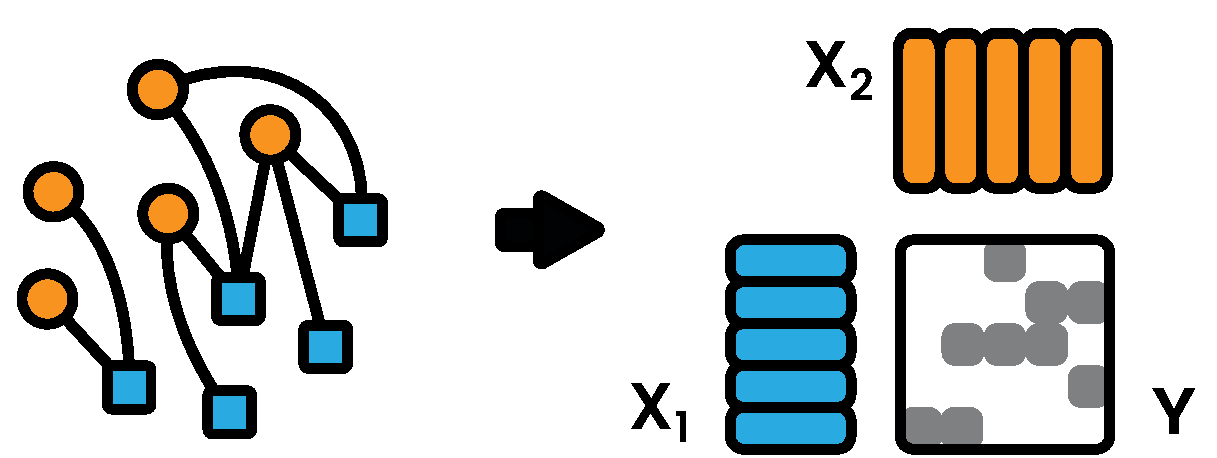
\includegraphics[width=.7\textwidth]{figures/bipartite_dataset.pdf}
    \caption{Representation of a bipartite network and its corresponding dataset.\newline Source: By the author.}
    \label{fig:bipartite dataset}
\end{figure}

Another important characteristic of our learning problems is that only the positive labels ($y=1$) are reliable. This means that an interaction between two instances may occur in reality even if annotated as negative ($y=0$) in the dataset. The datasets are thus termed positive-unlabeled (PU)~\cite{bekker2020learning}.

% TODO
%We use $\hat Y$, $\hat{\y}$ and $\hat y$ when referring to the final binary predictions of our models, while $\tilde{Y}$, $\tilde{\y}$ and $\tilde y$ are used for predicted probabilities.

%Our goal is to model a function $f \colon (\x_1,\; \x_2) \mapsto y$. $\x_1 \in \mathbb R^{m_1}$  $\x_2 \in \mathbb R^{m_2}$ are feature vectors of two interacting instances. $y \in \{0,\; 1\}$ is the label of their interaction.


%This includes a plethora of real-life phenomena, such as {...}.
% define sample/instance

%The known input vectors are usually organized as rows of an $X$ matrix so that
%$X\el{ij} = \x_i\el j$, and we refer as \emph{feature} or \emph{attribute} to
%each specific horizontal position $j$ of $x\el j$, which corresponds to a column
%of $X$. Likewise, a $Y$ matrix is built with their corresponding outputs
%($Y\el{ik} = y_i\el k$), also called \emph{targets} or \emph{labels}.

%Commonly referred to as "targets" in the context of regression learning, we here call the known outputs of the modeled process by \emph{labels}, as in classification, even if real-valued, to avoid confusion when referring to the protein targets of a drug.

%In the present setting, we concentrate on problems involving the interaction of
%two domains of instances (also called sample groups). As such, each sample
%domain forms a different $X$ matrix, that we term $X_1$ and $X_2$. Only
%inter-domain interactions are allowed, that is, instances are restricted from
%interacting with others in the same sample group, so that the interaction
%network constitutes an undirected bipartite graph.
%
%Each interacting pair of instances is also called a \emph{dyad}.

%The output, in our case, is any scalar piece of information describing the
%interaction between a given instance pair, such as the rating of a movie given
%by a user or a kinetic parameter of an enzyme-substrate reaction.
%We call these datasets \emph{bipartite}, to differentiate from the more common \emph{traditional} problems, in which a single $X$ matrix is utilized.
%We call these datasets \emph{bipartite}, to differentiate from the more common problems in which a single $X$ matrix is utilized.

%PU data, binary, drug-target

%Train test

% Let $X_a$ be a feature matrix, the index $a$ representing each the two
% bipartite sets of instances, such that each instance is written $X_a \el i\;
% \forall\; i \in \mathbb N,\, 1 \le i \le |X_a|_i$ and each instance's feature
% is denoted $X_a\el{i, j} \;\forall\; j \in \mathbb N,\, 1 \le j \le |X_a|_j$.
% Since data is bipartite in the setting we are considering, $a$ can only assume
% the values $1$ or $2$.

% Let $Y$ be the $(n_{1s}, n_{2s})$ labels matrix such that the element $Y\el{i,
% j}$ characterizes the interaction occurring between the instances $X_1\el i$
% and $X_2\el j$.

% $X$ in algorithms is $X_\text{SGSO}$ or ... all info about X

% RELATED TERMS section TODO
% \cite{liu2017computational} pu dyadic prediction
%one-class classification
%While \emph{link prediction} and \emph{dyadic prediction} are common terms in the literature referring to similar concepts, they are not specific to the presence of two distinct groups of objects nor make clear the presence of describing attributes for both of them (often called \emph{side-features} or \emph{side-information} in the context of recommendation systems). While \emph{interaction prediction} seems a closer alternative,
%usually assuming side-features, % TODO I do not think so
%it is also not concerned with the heterogeneity of the network.
%As an abuse of terminology, we thus refer to this "heterogeneous bipartite interaction prediction" paradigm as \emph{bipartite learning}.


\section{Data-centric adaptations of learning algorithms}
\label{sec:standard adaptations}

%As previously stated in \autoref{sec:problem_statement},
As discussed in \autoref{sec:approaches},
bipartite interaction problems fundamentally differ from the usual machine learning paradigm, in which input data represents a single entity to be labeled. Interaction tasks are instead concerned with labeling a relationship between two entities, and as such, each prediction is made upon a pair of feature vectors, each vector being specific to each of the two sample domains.

Such subtlety is often bypassed by reformulating a bipartite dataset into the traditional machine learning setting~\cite{vert2008reconstruction,schrynemackers2015classifying,pahikkala2015more}.
%
These strategies can be encompassed under two general approaches,
termed \emph{global} and \emph{local}~\cite{vert2008reconstruction,lu2011link,pahikkala2014twostep,pliakos2018global,pliakos2020drugtarget}.  %TODO cite more
%initially termed \emph{global} and \emph{local} \citeonline{vert2008reconstruction} and later adopted and extended by \citeonline{sschrynemackers2015}.  %TODO cite more
%
% TODO maybe direct citation to specify our changes
For the sake of clarity and generality, we further specify these categories by defining \emph{global} and \emph{local} as general properties of estimators, rather than specific training procedures:
%
\begin{itemize}
    \item \emph{\textbf{Global}} estimators are those aware of both instance domains during the training procedure ($X_1$ and $X_2$).
    \item \emph{\textbf{Local}} estimators are those which only have access to feature information from one of the two instance domains during training (either $X_1$ or $X_2$).
    As such, they are often employed in compositions, combining the predictions of several local models to produce the final output.
\end{itemize}
%
%We refer to \emph{traditional} estimators as those who are not specifically designed to deal with bipartite data, and \emph{bipartite} estimators as those who are. This distinction is important to differentiate between estimators that are naturally able to deal with bipartite data and those who are not, but can be adapted to do so.
Furthermore, to be consistent with \cite{schrynemackers2015classifying,pliakos2018global,pliakos2019network,pliakos2020drugtarget}, we assume the following definitions in our current context of bipartite interactions:
%
\begin{itemize}
    \item \emph{\textbf{Single-output}} estimators are those which consider all labels, i.e. all $Y\el{ij}$ elements, irrespectively of the column $j$ or row $i$ they are in. They are all regarded as a \emph{single type of output}.
    \item \emph{\textbf{Multi-output}} estimators, on the other hand, are those which consider each instance, each row or column of $Y$, as a separate task, for example by defining a composite loss function formed by the combination of losses over each row or column.
\end{itemize}
%TODO another term for multi-output, please. This is too confusing with multi-output in the traditional sense. bipartite multi-output are local models that use multi-output traditional estimators? or 3D interaction matrices with multiple labels for each interaciton?
Notice that the label matrix $Y$ can still be represented in two dimensions even if the model is single-output in this sense, contrary to the usual case where bidimensionality of $Y$ is a defining characteristic of a multi-output problem.

Finally, the two most common ways of adapting traditional estimators to bipartite data are then named \emph{global single-output} (GSO) and \emph{local multi-output} (LMO), as proposed by \citeonline{schrynemackers2015classifying}. We further denote them \emph{standard}, to clearly distinguish them from new adaptation proposals that could share the globality, locality, or outputness properties, but work in an entirely different way.
%
Specific definitions and shortcomings of these procedures are now presented.


\subsection{The standard global single-output adaptation}
\label{sec:sgso}

% TODO define SGSO acronym
%TODO literature (ben-hur? vert? pliakos? schynemackers?)
%Arguably the most straightforward and commonly used bipartite adaptation strategy
Arguably the most straightforward way to provide bipartite data into a conventional learning algorithm 
%strategy for adapting bipartite data to
%be inputted into
%conventional estimators.
%is through presenting concatenated pairs of row-column samples, labeled by each element of $Y$.
is by presenting concatenated pairs of row-column samples, labeled by each element of $Y$.
%
% The interacting dyad itself is what we abstract as a sample in this case.
The interacting dyad is now what we consider a sample, and each feature vector is the combination of the feature vectors of the two interacting instances.
% , and each feature vector is the combination of the feature vectors.
This is usually done by converting the two $X$ matrices and the
interaction matrix $Y$ to a single design matrix we call $X_\text{SGSO}$ and a column-vector of labels we refer to as $Y_\text{SGSO}$.

One way of doing so is by choosing indices as described by \autoref{eq:gsodata}, where
all combinations of $i_1$ with $i_2$ are explored (see \autoref{fig:sgso}).
%$f\colon (X_1\el{i\cdot},\; X_2\el{k\cdot}) \mapsto Y\el{ik}$.  To make use of
%traditional learning algorithms, one would combine instances from both $X_a$
%sets in a matrix we hereafter call $X_\text{SGSO}$, where each row is built by
%concatenating a row from $X_1$ followed by a row from $X_2$. $Y_\text{SGSO}$ can then
%take the shape of a one-dimensional column vector labeling each instance pair,
%as usual for single-output problems.

%This way of formatting interaction datasets is named by \ref{pliakos2018} as
%\emph{global single output} (GSO) scenario, and a possible definition is
%presented by \ref{eq:gsodata}, where $\lceil \cdot \rceil$ is the ceil function
%and $\concat$ denotes vector concatenation.
%
\begin{equation}  % TODO use m instead of |X|
    \begin{split}
    i_g &= (i_1-1)|X_2|_i+i_2-1\\
    X_\text{SGSO} \el{i_g} &= \begin{bmatrix} X_1 \el{i_1} & X_2\el{i_2}\end{bmatrix}\\
    Y_\text{SGSO} \el{i_g1} &= Y\el{i_1i_2}
    %X_\text{SGSO} \el{i} &= X_1 \el{\lceil i/|X_1|_j \rceil} \concat X_2\el{i \mod |X_2|_j}\\
    %Y_\text{SGSO} \el{i} &= Y\el{\lceil i/|X_1|_j \rceil,\; i \mod |X_2|_j}
    \end{split}
    \label{eq:gsodata}
\end{equation}

\begin{figure}[tb]
    \centering
    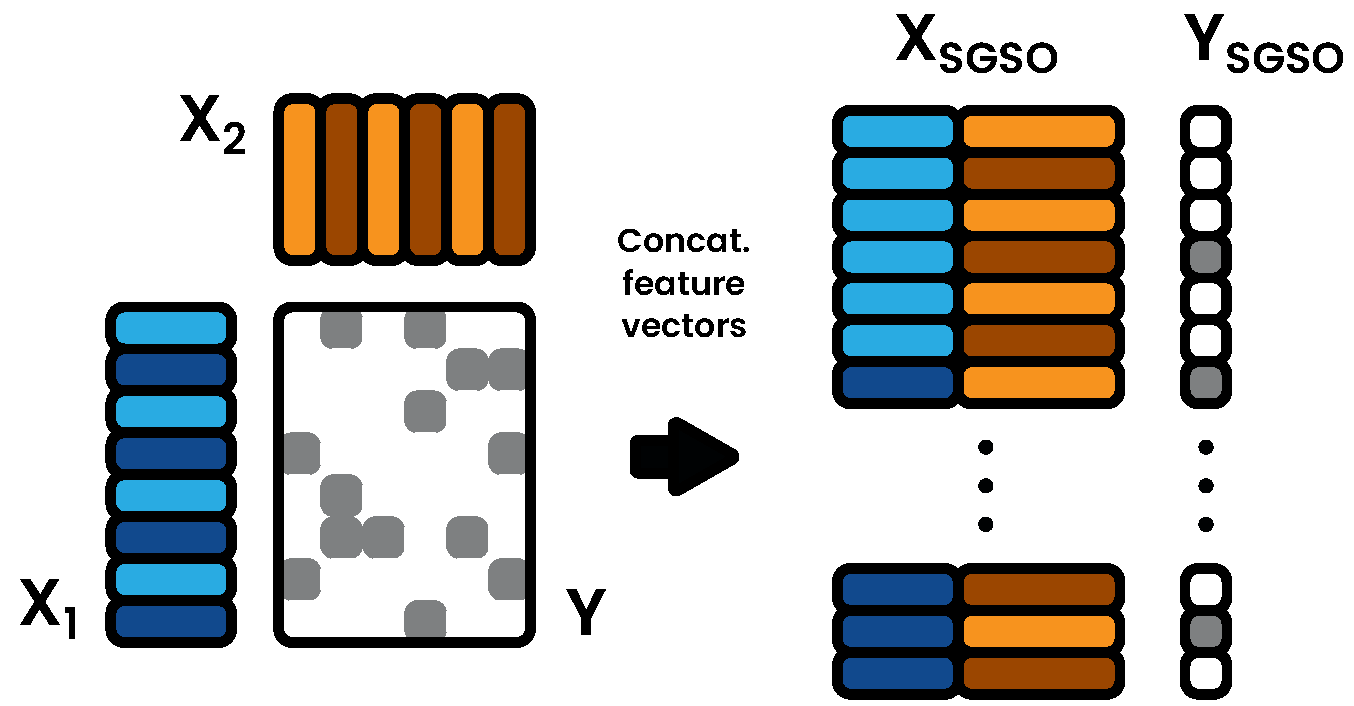
\includegraphics[width=.5\textwidth]{figures/gso.pdf}
    \caption{
        The standard global single-output (SGSO) approach. The bipartite dataset is represented as two matrices $X_1$ and $X_2$, and a matrix $Y$ of shape $|X_1|_i$ by $|X_2|_j$. The SGSO approach concatenates the rows of $X_1$ and $X_2$ to form a new feature matrix, in which each row represents a dyad. The interaction matrix $Y$ is then reshaped into a column vector, so that each element of $Y$ is associated with a row of the new feature matrix. The resulting dataset is then used to train a conventional single-output estimator.
        \newline Source: By the author.
    }
    \label{fig:sgso}
\end{figure}


To consider all possible dyads, $X_\text{SGSO}$ would have $|X_1|_i|X_2|_i$ rows and $|X_1|_j+|X_2|_j$ columns. Thus, $X_\text{SGSO}$ as defined by \autoref{eq:gsodata} is highly redundant.
%Reformatting $Y$ has no impact in memory usage, with $Y_\text{SGSO}$ having a single column but all the same $|X_1|_i|X_2|_i$ elements as $Y$.
%However, as stated in section \ref{sec:definitions}, $X_\text{SGSO}$ would be a $|X_1|_i|X_2|_i$ by $|X_1|_j+|X_2|_j$ matrix if one intends to consider all interactions in $Y$, which
As a result, dealing with such a large $X_\text{SGSO}$ matrix is impeditive in many cases, both in terms of memory usage and computation time. Therefore, a commonly used workaround is to undersample the negative annotations, yielding a dataset with equal amounts of positive and negative interactions~\cite{ozturk2018deepdta,huang2020moltrans}.
This strategy is justified by the negative-annotated dyads being usually far more numerous than positives and much more likely to be truly negative interactions than false negatives.
%Despite such reasoning, we demonstrate in \autoref{} that taking all negative samples into consideration instead has significant benefits, and we propose new model optimizations to enable it (\autoref{}).
Nonetheless, we demonstrate in \autoref{sec:adaptation_comparison} that undersampling negatives is significantly detrimental if the main goal is to indicate wich interactions are most likely to be true.

% TODO cross-validation is naively done

\subsection{The standard local multi-output adaptation}
\label{sec:slmo}

The local approaches, in contrast to global methods, propose training different models on $X_1$ and $X_2$, so that each estimator only has access to information regarding either row samples or column samples.

As such, multiple non-bipartite models need to be used in conjunction to predict interactions between new row samples and new column samples. The standard local multi-output (SLMO) approach uses two traditional estimators for each axis (four in total), that we here refer to as \emph{primary} and \emph{secondary} estimators.
In general, they must be multi-output estimators, each being able to output a bidimensional $Y$ matrix.
%receive $X_\text{train}$ and $Y_\text{train}$ bidimensional matrices in the training step, receive an $X_\text{new}$ in the prediction step such that $|X_\text{new}|_j=|X_\text{train}|_j$, and outputting $Y_\text{pred}$ with $|Y_\text{pred}|_i=|X_\text{new}|_i$ newly predicted rows and $|Y_\text{pred}|_j = |Y_\text{train}|_j$ output columns.

The procedure for training the estimators in an SLMO setting consists of simply training the primary estimators. The primary rows estimator is trained on $X_1$ and $Y$, and the primary columns estimator on $X_2$ and $Y^\intercal$ (\autoref{alg:train_local_model}). The prediction step is however more complicated, involving the training of the secondary estimators on predictions of the primary models.
The procedure is described in details by \autoref{alg:predict_local_model} and illustrated by \autoref{fig:slmo}. The \KwCombine function used in line \autoref{ln:combine_local_outputs} of the \autoref{alg:predict_local_model} procedure can be arbitrarily chosen, and is usually defined as the simple element-wise average of both matrices (\KwCombine{$Y_1$, $Y_2$} $= \frac{1}{2}(Y_1 + Y_2)$).

\begin{figure}[tb]
    \centering
    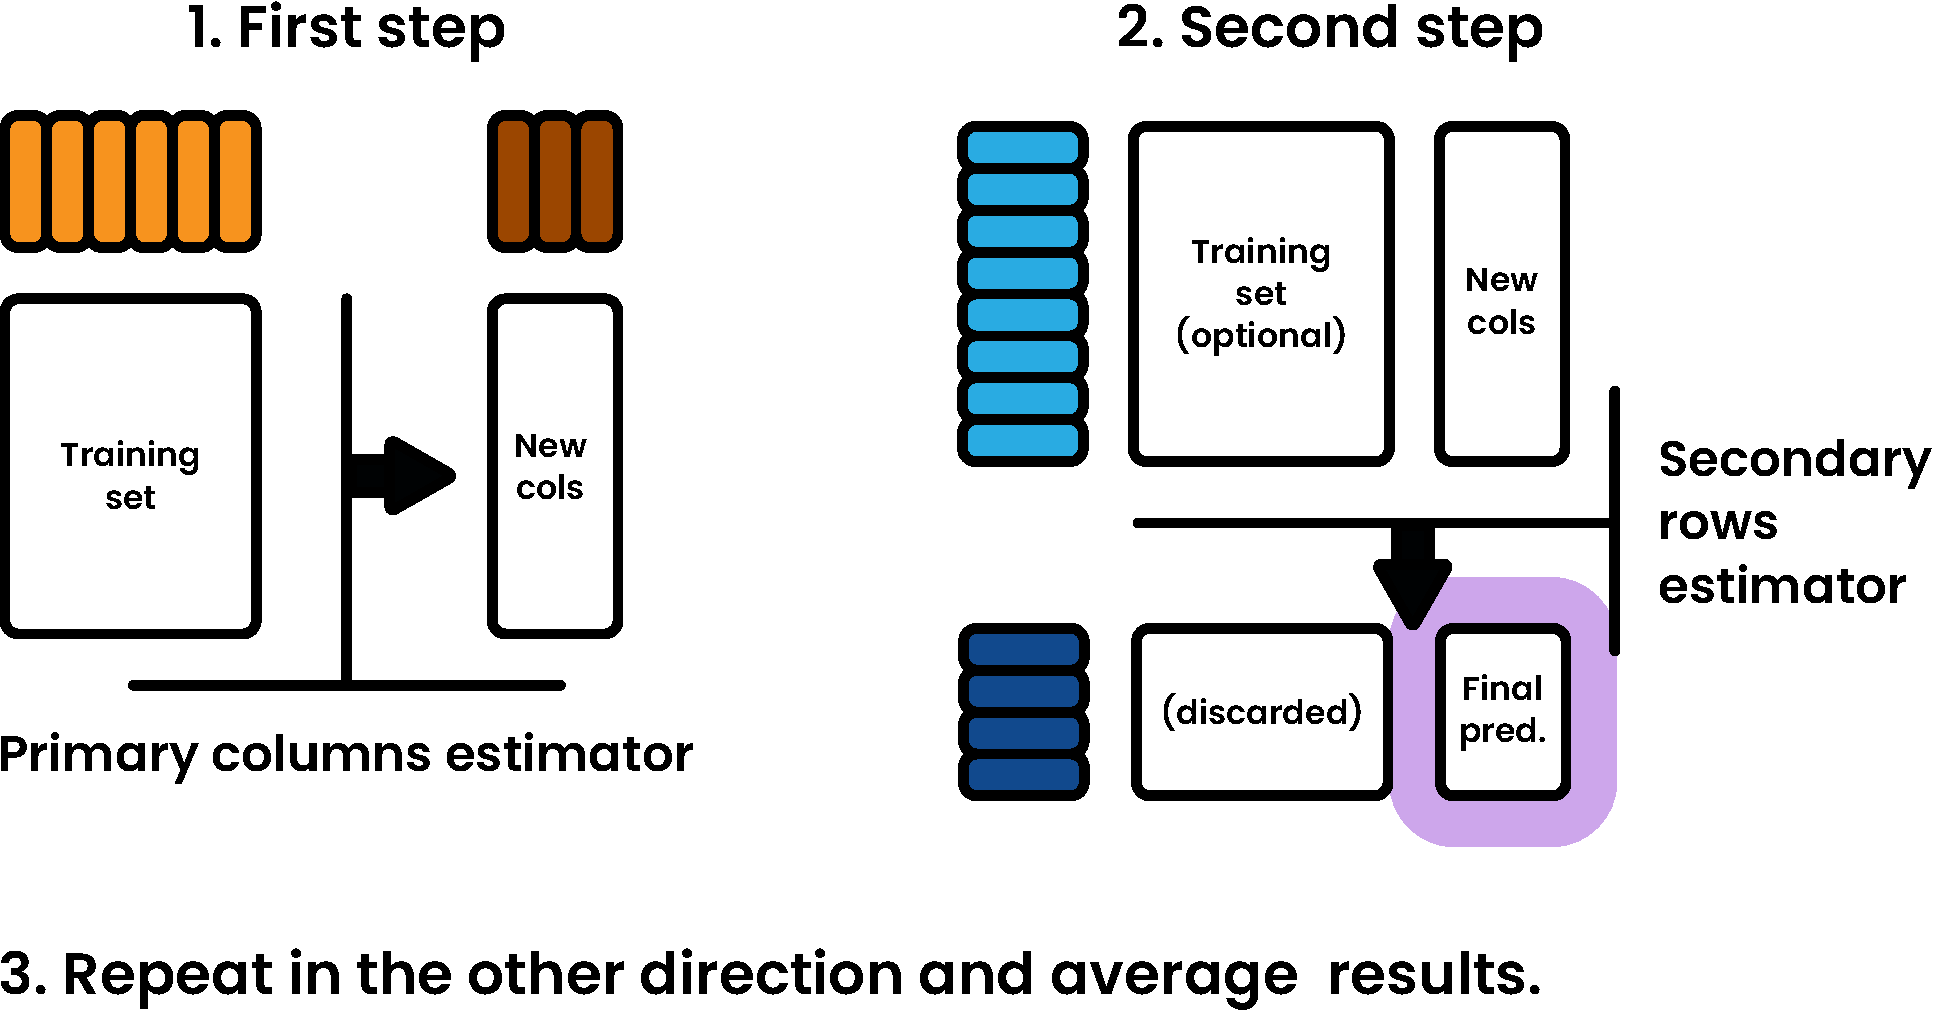
\includegraphics[width=.6\textwidth]{figures/lmo.pdf}
    \caption{
        The standard global single-output (SLMO) approach. The bipartite dataset is represented as two matrices $X_1$ and $X_2$, and a matrix $Y$ of shape $|X_1|_i$ by $|X_2|_j$. The SLMO approach trains two primary multi-output estimators, one for each axis, and then trains two secondary multi-output estimators on the predictions of the primary models. The secondary models are then used to predict the interactions between new row samples and new column samples.
        \newline Source: By the author.
    }
    \label{fig:slmo}
    %\caption{Illustration of the training procedure under the local multi-output approach for adapting traditional learning algorithms to bipartite data. To be able to predict interactions among completely new sample pairs, this approach aggregates four multi-output monopartite estimators. In a first step, a primary rows estimator is trained on X_0 and y, and a primary columns estimator on X_1 and y.T. The predictions of the primary estimators are used to extend the interaction matrix, as shown as the step 1 in figure (only the columns estimation is shown). The extended matrix then is used to train a secondary rows estimator and a secondary columns estimator. Finally, the predictions of both secondary estimators are arbitrarily combined to yield the final predictions (the most common combination method is taking the simple average between both axes). Note that, although not necessary, one may consider using the training set also when training the secondary estimators, if these estimators are able to take advantage of possible cross-output inter-dependencies.}
\end{figure}

%, optionally combined with the original training data

\algTrainLocalModel
\algPredictLocalModel

An unusual behaviour occurs if the secondary estimators are able to exploit inter-output dependencies. In this case, the outputs of the SLMO composition would depend on the amount of test data and specific combinations of test instances provided. This is usually not the case in traditional learning problems, and complicates the evaluation procedure. The behaviour forces us to consider the size and sampling method of the batches of test data. For online aplications, the ideal strategy would be to retrain the secondary models for each batch of new instances, using the predictions from the primary models over all the previously received instances (labeled and unlabeled). As a result, the application of SLMO models is effectivelly restricted to offline learning contexts.

%Notice that, if the secondary multi-output estimators treat each label independently, including the $Y_\text{train}$ labels in their training will make no difference, and one should use only the predictions from the primary estimators.

%A specific case of a model with multiple independent-outputs occurs when a collection of single-output models is utilized as a unified entity, each being trained on each column of $Y_\text{train}$.

%% This setup was present in the first proposal of a local model \cite{}, and enables a wider range of learning algorithms, not just multi-output strategies, to be employed in interaction prediction.  (WRONG)
%
%On the contrary, if the secondary estimator can exploit inter-output dependencies, one might consider concatenating the primary estimators' predictions to $Y_\text{train}$ and use both to train the secondary estimators (see lines \ref{} of Function \ref{alg:predict_local_model}). This setting would enable the secondary models to explore the output relationships involving the original training set, which are arguably more reliable than those between the primary predictions alone.
%
%That said, another consideration regarding the use of dependent-outputs secondary estimators is whether or not to provide the whole $X_{1\text{new}}$ and $X_{2\text{new}}$ at once, since doing so would increase the amount of primarily-predicted data used to train the secondary estimators, and it may be desirable to have more columns coming directly from $Y_\text{train}$ rather than inferred by the primary models. The ideal scenario then would be to run \ref{alg:predict_local_model} once for every $X_{1\text{new}}$ and $X_{2\text{new}}$ row combination, in a total of $|X_{1\text{new}}|_i|X_{2\text{new}}|_i$ iterations, with possible performance drawbacks for most learning algorithms. The natural intermediate idea would be to provide $X_{1\text{new}}$'s and $X_{2\text{new}}$'s rows in batches, possibly increasing the prediction time but ensuring the $|X_{a\text{new}}|_i/|X_{a\text{train}}|_i$ ratio is not detrimentally high. Additionally, some algorithms allow for output weights to be used in the training procedure, enabling us to assign lower importance to the $Y_{\text{new}}$ columns inferred by the primary estimators.
%
%In any case, contrary to what is usually observed, the amount of test data and specific combinations of test instances provided to the SLMO ensemble clearly affect the resulting predictions when the secondary models have inter-dependent outputs. This characteristic should thus be taken into consideration when developing, evaluating and comparing bipartite estimators under the SLMO configuration, although seldomly addressed by previous authors in our experience.%TODO: harsh?
%
%Due to each traditional model being provided with a much lower number of instances in comparison to the SGSO procedure, SLMO models tends to be naturally faster to train than SGSO models. However, a striking limitation of the SLMO procedure is caused by its inference phase, which requires traing of the secondary models whenever new instances are inputted. The resulting large prediction times hinders the application of SLMO models on online learning scenarios.
%
% problems of predicting.

%provide examples of each case (dependent vs independent outputs)
% we try to join multiple similar ideas under a single framework

%The idea was first proposed by \cite{}, and \cite{} expanded the concept to multioutput models to predict completely new pairs. The \cite{}

%examples of estimators in each category DNLMF, DNILMF BLM BLM-NII, etc.

%list characteristics of each main category:
% gso receives x1x2 lines
% matrix reconstruction algs dont predict by themselves

%\section{Bipartite decision forests}
%\label{sec:bipartite forests}
%
%%A \textit{sui generis} learning algorithm adaptation was proposed by \citeonline{pliakos2018} to deal with bipartite data, without the need for dataset reformatting as in SGSO, or compositions of multiple estimators and secondary training steps as SLMO.
%
%%
%
%
%%Named Predictive Bi-Clustering Tree (PBCT) by the authors, it tunes the usual decision tree-growing algorithm to directly operate on bipartite interactions, building a single tree model directly on bipartite formatted datasets (using $X_1$, $X_2$ and $Y$). Importantly, their proposed algorithm inherits all the benefits of tree-based estimators, such as their well-known interpretability and remarkably low amount of hyperparameters~\cite().
%%
%%
%%Intriguingly, PBCTs were only explored in a scarce number of previous studies~\cite{pliakos2018global,pliakos2019network,pliakos2020drugtarget}, to the best of our knowledge. A possible explanation is that no improvement in computational complexity of training times is observed with respect to SGSO-adapted decision trees~\cite{pliakos2018global}, even if drastically less memory is used by a PBCT in comparison to a naive implementation of SGSO.  %TODO more pbct papers
%%Furthermore, no implementations of PBCTs are provided in sufficiently accessible and extensible formats, which could also have hindered its adoption by the scientific community.
%%
%%We thus turn our attention onto such tree-based algorithms, proposing optimizations proven to reduce asymptotic training times of bipartite trees by a $\log |X|_i$ factor, enabling larger bipartite datasets to have all its unknown (0-labeled) interactions considered in model training and bringing unprecedented scalability to tree and forest estimators on interaction prediction tasks.
%%%Intriguingly, these estimators were only explored in a scarce number of previous studies\cite{}. We thus turn our attention onto them, proposing optimizations to enable all unknown interactions to be considered in training, so to bring unreported scalability of Random Forests in sparse problems of interaction prediction and recommendation.
%%
%%%TODO we made them accessible, bipartite_learn
%%


%\subsection{Traditional decision trees}  % TODO traditional?
%\subsection{General decision trees}
\section{Decision trees}
\label{sec:dt}
%TODO describe origin and benefits of trees
% decision tree (DT)
% more accessible intro

A general description of top-down decision trees is now presented, as a theoretical foundation for the upcoming formal definition of bipartite decision trees (\autoref{sec:bipartite_trees}).

Let's consider the scenario where a single protein of interest is selected, and we receive the task of determining which drug molecules will likely affect its physical structure or catalytic function.
We wish to find a systematic procedure to decide whether a given drug molecule $\x_i$ will interact with our protein or not. To develop such a procedure, consider we have at our disposal a set of $m$ known drug molecules, whose degree of interaction with our protein of interest was previously experimentally determined. We can then describe a drug molecule $\x_i$ in general by how similar it is to each of our $m$ known molecules, organizing this information as a vector $\x_i = \begin{bmatrix}\x_i\el{1} & \x_i\el{2} & \x_i\el{3} & \cdots & \x_i\el{m}\end{bmatrix}$ so that $\x_i\el{j}$ represents the similarity score between the drug $\x_i$ and the $j$-th of our $m$ known drugs.

The hypothetical decision procedure we intend to determine could then be structured as a path with consecutive bifurcations. We always start at the same place, and, at each bifurcation, a question is asked about the drug $\x_i$ in hands. The questions are in a standard format, exemplified by "Is $\x_i$ more than 60\% similar to the 3\textsuperscript{rd} known drug?", or $\x_i\el{j} > t$, for a general known drug $j$ and similarity threshold $t$. The answer to the question in each bifurcation determines which of the two possible paths we should follow. No cycles are allowed in the path, and eventually, all routes reach final locations instead of bifurcations. Each final location contains a fixed value that will be returned as the final decision about the drug $\x_i$'s effect on our protein of interest.

Such a decision procedure, structured as a binary tree path, is what is commonly referred to as a \emph{decision tree} (DT) model~\cite{breiman1984classification}, illustrated by \autoref{fig:dt}. 
In this context, each bifurcation then represents a tree \emph{node}, and the final locations are called \emph{leaves}. The value outputted by each leaf is termed the leaf's \emph{prototype}.
%
%The well-known interpretability of decision trees results from these
%rules leading to each output being clearly defined along the tree structure
%is what results in the well-known transparency of decision trees, an attractive characteristic in fields such as drug discovery or regulatory network inference, where insights into the underlying processes are greatly valued.

%The described binary-tree structure is by far the most utilized~\cite{}, being ubiquitous to all tree-based estimators in the present study.

The main challenge, however, lies in the building process of such models: in how to determine the rules that define each fork and how we define the stopping criteria for a final decision to be yielded.

%As presented by \autoref{sec:definitions},
To build the decision tree, we are given a training set composed of the two bidimensional matrices $X$ and $Y$. The dataset represents $|X|_i = |Y|_i$ instances, each described by $|X|_j$ numeric features and labeled by $|Y|_j$ labels.
In the previous example, $|X|_i$ would be the number of drug molecules in the dataset
$|X|_j$ would be the number of reference drugs (used to obtain the similarities), and $|Y|_j$ would be the number of proteins of interest.

%(drug molecules in the previous example)

%so that $X\el{i} = \x_i$ represents the $i$-th entity. Each entity is thus described by $|X|_j$ numeric descriptors (similarities to known drugs in the previous example). To each entity is assigned one or more numeric labels $Y\el{i}$ describing the known target prediction results. In analogy to the last example, the labels would denote interaction or not with one or more proteins of interest.

Consider now executing the prediction process of a decision tree for each training instance, going through the branched path. Each bifurcation would divide the training instances between those who answer the question affirmatively and those who answer negatively. Eventually, each leaf will contain a partition of the training instances.
From the resulting partitions, we can evaluate the decision tree:
a "good" decision tree would be one in which the prototype value of each leaf is a good estimate of the labels in the leaf's partition.
%
The training algorithm then approaches the problem from the other direction: what would be a good tree according to our training data?
A greedy top-down procedure is usually followed, that we introduce bellow.
%This evaluation is used by the training procedure to evaluate each candidate splitting rule. The best rules are selected 
%The training procedure uses such evaluation to determine the best possible splitting rules. The tree is built 

%The procedure for building a DT consists of determining features $f$ and threshold values $t$ that recursively split the dataset in two parts, named \emph{left} and \emph{right} partitions, as defined by \autoref{eq:datasplit}.
Formally, each rule is encoded by an index $f$ representing a feature column and a threshold value $t$. Each rule then represents a split of the training dataset in two partitions, named \emph{left} and \emph{right}, as defined by \autoref{eq:datasplit}.
%
\begin{equation}
    \begin{split} %TODO
        %Y_\text{left} &=\{Y\el{k\cdot} \;\forall\; k \mid X\el{kf} \le t\}\\
        %Y_\text{right} &=\{Y\el{k\cdot} \;\forall\; k \mid X\el{kf} > t\}\\
        %X_\text{left} &=\{X\el{kf} \;\forall\; k \mid X\el{kf} \le t\}\\
        %X_\text{right} &=\{X\el{kf} \;\forall\; k \mid X\el{kf} > t\}\\
        Y_\text{left} &=Y\el{(X\el{if} \; \le \; t)} \\
        Y_\text{right} &=Y\el{(X\el{if} \; > \; t)} \\
        X_\text{left} &=X\el{(X\el{if} \; \le \; t)} \\
        X_\text{right} &=X\el{(X\el{if} \; > \; t)}
    \end{split}
    \label{eq:datasplit}
\end{equation}

To build a decision tree, we start with the whole training set (the \emph{root node}). A procedure FindSplit is executed to yield a good splitting rule.
The training data is then partitioned according to this rule, as defined in \autoref{eq:datasplit}. Two descendant nodes are created, each receiving one of the partitions.
For each new node, we have two options: i) apply FindSplit to its data partition and continue recursively; or ii) set the node as a leaf, taking record of the partition it received.

The tree-building algorithms can thus be described by four key components:
%
\begin{enumerate}
    \item \textbf{The FindSplit procedure}, which determines a set of candidate splitting rules and selects the best one according to a quality metric.
    \item \textbf{The split quality metric} used by FindSplit to evaluate the candidate rules.
    \item \textbf{The stopping criteria}, that determine when a node should be set as a leaf.
    \item \textbf{The prototype function}, that determines the output value of a leaf.
\end{enumerate}
%
\autoref{alg:buildtree} describes in detail how these components come together to build a decision tree. \autoref{alg:predict} then formally details how predictions are made given a model built by \autoref{alg:buildtree} and a new data instance.
%
These procedures emcompass a wide range of decision tree algorithms, including the popular CART ~\cite{breiman1984classification}, ID3~\cite{quinlan1986induction}, and C4.5~\cite{quinlan2014c4}, as well as the bipartite trees we explore in the present work~\cite{pliakos2018global}.  %TODO VERIFY

The following sections provide further considerations on specific components.

\algPredict
\algBuildTree

%For each new node, we have two options: can either apply FindSplit to its data partition, or set the %node as a leaf, taking record of the partition it received.
%For each new node, we can either apply FindSplit to its data partition, or set the node as a leaf, taking record of the partition it received.

%For each partition, the same procedure is repeated, until a stopping criterion is met. The most common stopping criteria are a maximum depth of the tree or a minimum number of samples in a node, for instance.
%
%Each child node receives one of the data partitions generated by its parent, and the process is recursively repeated until a stopping criterion is met. The most common stopping criteria are a maximum depth of the tree or a minimum number of samples in a node, for instance.
%Each bifurcation of a DT, more commonly referred to as a \emph{node}, then represents one of such splits, defined by a selected feature $f$ and a threshold value $t$, and each of its two children receives one of the data partitions generated by its parent (see \autoref{}). Under specific pre-defined circumstances, a node stops generating descendant nodes, having no children and taking record of the dataset partition it received from its parent. Among possible stopping criteria are a maximum depth of the tree or a minimum number of samples in a node, for instance. These terminal nodes are called \emph{leaves}.

%We can also formally define the inference procedure illustrated in the introductory example.
%The prediction step for a new sample $\x_\text{new}$ consists of transversing the tree from the root node until a leaf, following each node's test ($\x_\text{new}\el{f_\text{node}} > t_\text{node}$).
%%and selecting the corresponding child node as given by the partitioning rule of \autoref{eq:datasplit}.
%Once a leaf is reached, the tree returns a prototype value calculated over the partition of the training data corresponding to that leaf. The average label ($Y_\text{leaf}^{\ang i [j]}$) of each output is a common choice for this prototype.
%


\subsection{Searching for the best split}
\label{sec:split search}

We explore two main strategies for the FindSplit procedure: the exhaustive search and the randomized search. The exhaustive search is the most common. The randomized search is a faster but less accurate alternative, intended to be used in the context of tree ensembles (\autoref{sec:decision forests}). We describe each procedure in the present section.

The most common approach to the FindSplit procedure is to consider all possible partitions of the given input data.
%
For a feature column $X\el{\cdot f}$, this exhaustive evaluation of partitions can be done by sorting $X\el{\cdot f}$ and considering a threshold $t$ between each two consecutive values in it. Notice that any threshold value between the same two consecutive $X\el{\cdot f}_\text{sorted}$ elements will result in the exact same partitioning of the training set (\autoref{eq:datasplit}). The common practice is thus to take the averages between each two neighboring feature values. The same procedure is then repeated for each feature column, and the overall best $t^\ast$ and corresponding feature index $f^\ast$ are selected.
%
%A greedy procedure is then followed for the overall tree growing, selecting at each node the best $t$ and $f$ to represent the split, according to a predefined quality criteria we further discuss in \autoref{sec:criteria}.
%
The exhaustive split search procedure is detailed by the \autoref{alg:find_best_split}.
%The algorithm \ref{alg:buildtree} then describes its application on growing a traditional decision tree (stablished by \citeonline{breiman1984classification}),
%while \ref{alg:predict} formally details how predictions are made given a model built by \ref{alg:buildtree} and a new data instance.

\algFindBestSplit

The randomized search is an alternative that avoids considering all partitioning options and greatly reduces the amount of operations performed.
It consists of drawing a random threshold $t$ between the minimum and maximum value of each feature, thus evaluating only $|X|_j$ splits when choosing the best (\autoref{alg:find_random_split}). Although degrading the performance of a single tree, this procedure is an interesting option when building tree ensembles (\autoref{sec:decision forests}), being the core idea behind the extremely randomized trees algorithm~\cite{geurts2006extremely}.  %TODO standardize alg names
Ensembles of decision trees will be discussed in \autoref{sec:decision forests}.

%\algSplitDataset
\algFindRandomSplit

%Notice that the described procedure requires us to sort the $X_\text{SGSO}$'s column corresponding to the $f$ feature ($X_\text{SGSO}\el {:,\,f}$), so that we can apply the same permutation that sorted $X_\text{SGSO}$ to $Y_\text{SGSO}$, yielding $X_{\text{permuted}}$ and $Y_{\text{permuted}}$, and generate the data split according to \ref{eq:sortedsplit}, being $i^*$ the index corresponding to the chosen threshold $t$ such that $t=\frac{1}{2}(X_{\text{permuted}}\el{i^*,\,f}+X_{\text{permuted}}\el{i^*+1,\,f})$.
%
%\begin{equation}
%    \begin{split}
%        X_l &= Y_{\text{permuted}}\el{:i^*}\\
%        X_r &= X_{\text{permuted}}\el{i^*:}\\
%        Y_l &= Y_{\text{permuted}}\el{:i^*}\\
%        Y_r &= Y_{\text{permuted}}\el{i^*:}
%    \end{split}
%    \label{eq:sortedsplit}
%\end{equation}

%prototypes

%\subsection{Split quality criteria and impurity metrics}
\subsection{Measuring the quality of a split}
\label{sec:criteria}

A split quality criterion must be defined so we can compare and select the best splitting rules at each node. The quality $\Delta I$ of a split is commonly framed as the decrease of an impurity metric calculated over the partitions of training labels (\autoref{eq:quality}). This decrease is taken for the combined impurities of the generated children nodes (\autoref{eq:datasplit}).
%relative to their parent's impurity.
All impurities are multiplied by the size of each partition relative to the total number of training samples ($|Y_\text{root}|$), restricting the effect of nodes with less data that could introduce spurious variations of impurity. Notice that $|Y_\text{node}|=|Y_\text{left}|+|Y_\text{right}|$.
% TODO: notice that |Y_a|_i / |Y_b|_i == |Y_a| / |Y_b|
%
\begin{equation}
    \Delta I(Y, t, f) =
        \frac{|Y_\text{node}|}{|Y_\text{root}|} I(Y_\text{node})
        - \frac{|Y_\text{left}|}{|Y_\text{root}|} I(Y_\text{left})
        - \frac{|Y_\text{right}|}{|Y_\text{root}|} I(Y_\text{right})
    \label{eq:quality}
\end{equation}

Several metrics can be chosen as the impurity function $I(\cdot)$, such as the Gini impurity, the Shannon entropy or the Poisson loss~\cite{breiman1984classification}.  % TODO CONFIRM CITATION
In this study we utilize the variance of each output column, averaged over all outputs (\autoref{eq:mse}). 
%
%labels as the basis for calculating a split quality parameter (\ref{eq:mse}). We also set the prediction output of a leaf node (given by the prototype function) to be the average of labels in the training set encompassed by the leaf. Therefore, the impurity $I$ of a dataset partition corresponds to the variance of its labels: 
%
\begin{equation}
    I_\text{MSE}(Y)
        = (Y\el{ij} - Y^{\ang i[j]})^{2\ang{ij}}
        = Y^{2\ang{ij}} - Y^{\ang i 2\ang j}
    %I(Y) = \avg{\left(Y\el{i, j} - \avg{Y\el{i, j}}\right)^2} \text{,}
    %%\text{MSE}(Y) = \avg{(Y\el{i, j} - \avg{Y\el{i, j}})^2} \text{,}
    \label{eq:mse}
\end{equation}
%
Most commonly, the \textt{prototype} function returns the column averages of a leaf's partition of the training labels: $Y_\text{leaf}^{\langle i\rangle[j]}$.
In this case, the column variances correspond to the \emph{mean squared error} (MSE) for the training data in the node, as if the node holding $Y_\text{partition}$ were to become a leaf.
%
% Derivation:
%
%\begin{multline}
%    I_\text{MSE}(Y)
%        = (Y\el{ij} - Y\mel i\el j)^2\mel{ij}
%        \\= (Y\el{ij}^2 -2 Y\el{ij} Y\mel i\el j + Y\mel i\el j^2)\mel{ij}=\\
%        = (Y\el{j}^2\mel i -2 Y\mel i\el j Y\mel i\el j + Y\mel i\el j^2)\mel{j}=\\
%        = (Y\el{j}^2\mel i - Y\mel i^2\el j)\mel j=\\
%        = Y^2\mel{ij} - Y\mel i^2\mel j
%    \label{eq:mse}
%\end{multline}

Also notice that $I_\text{MSE}$ is equivalent to the Gini impurity if $Y$ contains only binary values. That can be shown by noticing that $Y_\text{bin}^{[ij]2} = Y_\text{bin}\el{ij}$ for binary labels, so we define $\mathbf{p}$ as $\mathbf{p}\el{j} = Y_\text{bin}^{2\ang{i}[j]}=Y_\text{bin}^{\ang i [j]}$, which yields \autoref{eq:gini}.
%, culminates in the usual form of the average of Gini impurities across all outputs.
%
\begin{equation}
    I_\text{MSE}(Y_\text{bin})
        = Y_\text{bin}^{2\ang{ij}} - Y_\text{bin}^{\ang{i}2\ang j}
        = (\mathbf{p}\el j  - \mathbf{p}^{\ang j 2})\mel j
        = [\mathbf{p}\el j(1 - \mathbf{p}\el j)]\mel j
    = I_\text{Gini}(Y)
    %I(Y) = \avg{\left(Y\el{i, j} - \avg{Y\el{i, j}}\right)^2} \text{,}
    %%\text{MSE}(Y) = \avg{(Y\el{i, j} - \avg{Y\el{i, j}})^2} \text{,}
    \label{eq:gini}
\end{equation}

%Referring back to bipartite scenarios, we now describe how intuitive adaptations of the decision tree algorithm are developed to deal with interaction data.


\section{Bipartite decision trees}
\label{sec:bipartite_trees}

Some learning algorithms can be adapted in a deeper level to the bipartite context. These algorithms are able to directly receive the two $X$ matrices as input, without needing to combine them as a preprocessing step for training.  % TODO lmo?
We term them \emph{estimator-centric} adaptations, in contrast with the data-centric strategies discussed in \autoref{sec:standard adaptations}.  % TODO standardize names
%
% TODO benefits are in the intro
% TODO shortcommings: slow and not semisupervised
%
This section explores the main focus of this work: estimator-centric adaptations of decision tree models. \autoref{sec:estimator-centric} presents two other estimator-centric strategies, based on linear models and matrix factorization.

%In this section, we describe how the decision tree algorithm can be adapted to directly operate on bipartite interaction data.

Essentially, the adaptation process consists of defining bipartite versions of each of the four key components of the decision tree algorithm (\autoref{sec:dt}): the FindSplit procedure, the split quality metric, the stopping criteria, and the prototype function. From these, the most central is the FindSplit procedure adaptation.
%As presented by \autoref{sec:bipartite_forests}, \citeonline{pliakos2018global} introduces an ingenious strategy to build a decision tree directly on bipartite-formatted datasets.
 
For bipartite trees, as proposed by \citeonline{pliakos2018global}, we perform the split search locally in each domain, in a similar fashion to the SLMO adaptation (\autoref{sec:slmo}).
% but specifically for each tree node. 
%
%The main concept behind it borrows the idea of the SLMO approach described in \autoref{sec:slmo},
%in that the training procedure is divided into two steps, separately considering each axis of the bipartite data. However, instead of training two separate models as in SLMO, two candidate versions of each node are generated, one for each axis, and the best between both is selected to integrate the final model.
%
%Formally speaking, consider a general procedure \FindSplit for finding a split threshold in a traditional multioutput decision tree (see \autoref{sec:dt}).
Specifically, let \FindSplit\textsubscript{trad} be a procedure for finding a split threshold in a traditional multioutput decision tree (see \autoref{sec:split search}).
%The algorithm by \cite{pliakos2018global}
A bipartite tree applies \FindSplit\textsubscript{trad} twice at each node: once over $X_1$ and $Y$ and once over $X_2$ and $Y\T$. This results in one split being chosen for each axis.
Finally, the best overall split is selected between the vertical and horizontal splits.
%horizontal split and the vertical split.
%, according to the quality criterion of \autoref{eq:q_lmo}.
%, so that each $Y$ \emph{row} is now interpreted as an output.
%in which case each $Y$ \emph{column} is considered a different output;
In essence, a bipartite decision tree algorithm uses a \FindSplit procedure that composes two traditional \FindSplit\textsubscript{trad} procedures, as detailed by \autoref{alg:find_bipartite_split}.

%Although each node locally performs the partitioning search on each axis, the resulting tree in its entirety is termed \emph{Global MultiOutput} (GMO) by the original authors, and its training procedure corresponds to using \FindSplit = \ref{alg:find_bipartite_split} in \ref{alg:buildtree}.

\algFindBipartiteSplit

%\begin{equation}
%    I = I(Y) + I(Y\T)
%\end{equation}
%
%Interestingly, contrary to the other adaptation approaches of traditional machine learning algorithms (\autoref{sec:standard adaptations}), the PBCT procedure does not require using multiple traditional estimators and training steps (such as SLMO, \autoref{sec:slmo}) or converting bipartite datasets to the memory-expensive global format such as SGSO (\autoref{sec:sgso}). Nevertheless, considering each row or column of $Y$ as a separate output results that growing a PBCT still occurs in the same asymptotic time complexity of a decision tree under the SGSO adaptation (derived in \autoref{sec:complexity_analysis}). 
%
%Remarkably, we show that leveraging the single-output assumption (\autoref{sec:standard adaptations}) in the tree impurity calculation can simplify the bipartite local split searching procedure introduced by \citeonline{pliakos2018global}, yielding a new PBCT-based algorithm with expressive gains in training time efficiency. A formal description of our algorithm proposal is now presented.
%
%%Nevertheless, an argument could be made in opposition to this idea.
%
%%In some sense, a decision tree could be understood as an ensemble of trivial node-wise estimators, each predicting the mean of the training labels in its partition.
%
%%A decision tree training process could indeed be understood as a wrapper procedure around a simpler estimator. Within each node, the decision tree training searches for a way to separate the training samples into two complimentary partitions. Evaluating several of such splits, it is chosen the one which minimizes the variances of each of the two $Y$ partitions it generates. This could be interpreted as minimizing the mean squared error of a trivial estimator that outputs the mean of $Y$ values for any given input. Under this optics, a decision tree recursively searches for binary splits that most favor the performance of a wrapped estimator.
%%
%%Still under this interpretation, the PBCT algorithm then consists of applying to this simple estimator in each node a strategy that resembles the LMO adaptation discussed earlier. The search for the best split is executed locally, for each axis, and the best overall result is chosen between each axis' best.
%%
%%Although maybe a wrapper of a locally adapted trivial estimator, the tree structure generated after training has the exact same format as that of a traditional decision tree, so that the prediction procedure does not involve any training of component models as is expected with LMO-adapted models. Hence, these bipartite data-centric tree learning algorithms seem to not fit under any of the previously described categories, and we choose to inaugurate a third group we hereafter call \emph{native bipartite models}, encompassing estimators whose basic functioning is specifically designed to deal with interaction data in its bipartite format.

\subsection{Bipartite global single-output trees}
\label{sec:bgso_trees}
%Although being developed specifically to interaction data, the PBCT algorithm shows no improvement in training time complexity relative to the naive GSO approach, as derived in the Section \ref{sec:complexity_analysis}.

This section shows how we can grow bipartite trees more efficiently, making tree estimators more scalable to large bipartite datasets.

The original bipartite tree proposed by \citeonline{pliakos2018global} uses the impurity metric $I_\text{MSE}$ (\autoref{eq:mse}) to evaluate splits, so that the authors classify their technique as a \emph{Global MultiOutput} (GMO) estimator. \emph{Multi-output} because the impurity evaluates the average variance of each label column (or row), as if each column (or row) were a different output. \emph{Global} because each tree utilizes features from both feature domains for training (see \autoref{sec:standard adaptations}).
Their GMO trees, however, are shown to have the same algorithmic complexity as traditional decision trees trained with the SGSO adaptation. We demonstrate that faster training algorithms can be developed if we assume a single-output format under the context of bipartite trees. %instead of GMO, without .

%Notice that
The split rules as defined by \autoref{eq:datasplit} are agnostic to the specific arrangement of the bipartite data. They can be seamlessly applicable to either the ($X_\text{SGSO}$, $Y_\text{SGSO}$) format employed by the SGSO adaptation (\autoref{eq:gsodata}) or directly to the $X_1$, $X_2$ and $Y$ matrices.
Furthermore, the impurity at each node of an SGSO tree,
%$I(Y_\text{SGSO})$,
in many cases can be translated to the bipartite format. \autoref{eq:bipartite_gso_equivalence} describes such a translation of the MSE impurity presented by \autoref{eq:mse}.
%
\begin{equation}
    I_\text{MSE}(Y_\text{SGSO})
        = Y_\text{SGSO}^{2\ang{ij}} - Y_\text{SGSO}^{\ang i 2 \ang j}
        % = (Y_\text{SGSO}\T)^{2\ang i} - (Y_\text{SGSO}\T)^{\ang i 2}
        = Y^{2\ang{ij}} - Y^{\ang{ij}2}
    \label{eq:bipartite_gso_equivalence}
\end{equation}
% 
%We can then define $I_\text{GMSE}$ as in \autoref{eq:gso_mse}:
If we then define
%
\begin{equation}
    I_\text{GMSE}(Y) = I_\text{MSE}(Y_\text{SGSO})
        = Y^{2\ang{ij}} - Y^{\ang{ij}2}
    \label{eq:gso_mse}
\end{equation}
%
the exact same SGSO-adapted decision tree, with its node structure and split rules, can be grown by applying the bipartite procedure (\autoref{alg:find_bipartite_split}) with the $I_\text{GMSE}$ impurity instead of the original $I_\text{MSE}$. This again follows from the generality of the split rules defined in \autoref{eq:datasplit}, invariant under the SGSO data rearrangement (\autoref{eq:gsodata}).

%Notice how the divergence in \ref{eq:mse_gmo} is computed relative to the average of each $Y$ column, while in \ref{eq:gso_mse} the inner average is computed over the whole $Y$ matrix.

%Using this new impurity poses a simple yet sound advantage over the original. 
Notice how the squared divergences in \ref{eq:mse} is computed relative to the average of each $Y$ column, while in \ref{eq:gso_mse} the inner average is computed over the whole $Y$ matrix.  % TODO ?
%This highlights the key difference between GSO and GMO impurities: GSO considers all elements of $Y$ as different values for the same output.

We can explore this property of the GSO impurity to iterate more efficiently over candidate splits.
This is done by pre-computing averages of each row and column of $Y_\text{node}$. We can then iterate over one-dimensional $\tilde Y_\text{node}$ proxies (\autoref{eq:y_proxies}) instead of the bidimensional matrix when evaluating splits (\autoref{alg:find_best_split}).  %TODO indicate alg line
%
%Having only total averages in \autoref{eq:gso_mse}, always involving both $i$ and $j$ indices simultaneously, exempts the training function from storing column-wise label averages during split search, enabling us to pre-compute averages of each row and column of $Y_\text{node}$ and to iterate over one-dimensional $\tilde Y_\text{node}$ proxies (\autoref{eq:y_proxies}) instead of the bidimensional matrix when evaluating splits (\autoref{} of \autoref{alg:}).   % TODO REF ALGO
%
%This property can be explored to build a more efficient training procedure for bipartite GSO decision trees, as demonstrated in the asymptotic complexity analysis developed in \autoref{sec:complexity_analysis}.
%
\begin{equation}
    \begin{split}
        \tilde Y_1\el{i} = Y\el{i}\mel{j}\\
        \tilde Y_2\el{j} = Y\mel{i}\el{j}
        %\tilde Y_1\el{i} = \savg{Y\el{i,j}}_j\el{i}\\
        %\tilde Y_2\el{j} = \savg{Y\el{i,j}}_i\el{j}
    \end{split}
    \label{eq:y_proxies}
\end{equation}
%
The same is not possible for the GMO trees, as \autoref{eq:mse} requires storing averages for each $Y$ column, to be squared individually.
\autoref{alg:find_bipartite_split} describes the adapted procedure in each case.
%
The complexity improvements are demonstrated theoretically in \autoref{sec:complexity_analysis} and later empirically in \autoref{sec:empirical_complexity}.

% --------------
%However, in \autoref{eq:q_optimization} we demonstrate how a single-output impurity metric can be used directly in the bipartite setup. Being single-output, no distinction is made among $Y$ columns or rows, minimizing label deviance relative to the global average $Y\mel{ij}$ instead of column averages $Y\mel i\el j$. Considering such metric enables further optimization of the split searching procedure by employing single-column proxies of the interaction matrix (\autoref{eq:y_proxies}), as also described by the Function \ref{alg:find_bipartite_split} and justified in Section \ref{sec:complexity_analysis}.

% With the \ref{alg:find_best_split} procedure we intend to evaluate all possible data partitions with format as defined by \ref{eq:datasplit}.
%The bipartite decision trees grown with this procedure on $X_1$, $X_2$ and $Y$ have the exact same structure as a usual traditional decision tree trained on a dataset $X_\text{SGSO}$ and $Y_\text{SGSO}$ adapted with the traditional global strategy (Section \ref{}). This property can be intuitively shown by noticing that $X_1$ and $X_2$ already contain all the information necessary to define a set of thresholds that yields all possible partitions, since each partition considers a single $X$ column and building $X_\text{SGSO}$ does not removes or adds different elements to each of them (only repeats them).
%%and no conversion to the global traditional format ($X_\text{SGSO}$ and $Y_\text{SGSO}$) is necessary.
%This result is a consequence of \autoref{eq:gsodata} and is formally stated by \autoref{eq:bipartite_gso_equivalence}, in which we assume $f_2 = f_g-|X_1|_j$.
%
% \begin{multline}
%     \{Y_\text{SGSO}\el{k} \;\forall\; k \mid X_\text{SGSO}\el{k,\; f} < t\} =\\
%     \{Y_a\el{i,\; j} \;\forall\; i,j \mid X_a\el{i,\; f-(a-1)|X_1|_j}<t\}
% \end{multline}
% \[
% a=\begin{cases}
%     1, & \text{if} \;f \le |X_1|_j\\
%     2, & \text{otherwise}.
% \end{cases}
% \]
%\begin{equation}
%    \{Y_\text{SGSO}\el{k1}\;\forall\; k \mid X_\text{SGSO}\el{kf_g} < t\}
%    = \begin{cases}
%        \{Y\el{i_1i_2} \;\forall\; i_1\text{, }i_2 \mid X_1\el{i_1f_g}<t\}, & \text{if } f \le |X_1|_j\\
%        \{Y\el{i_1i_2} \;\forall\; i_1\text{, }i_2 \mid X_2\el{i_2f_2}<t\}, & \text{if } f > |X_1|_j
%    \end{cases}
%    \label{eq:bipartite_gso_equivalence}
%\end{equation}
%https://www.overleaf.com/project/62fbafab63095e6cfcb9a8ec


%As a result, we can substitute the procedure \ref{alg:find_best_split} by the wrapper procedure \ref{alg:find_bipartite_split} to efficiently build decision trees on bipartite data, directly using the much more compact $X_1$ and $X_2$ feature matrices rather than constructing the $X_\text{SGSO}$ GSO representation. A theoretical complexity analysis is presented by the section \ref{sec:complexity_analysis}.

%\begin{align}
%\begin{split}
%    & I(Y) =
%        \avg{(Y\el{i,j} - \savg{Y\el{i,j}})^2} =\\
%        &=\avg{(Y\el{i,j})^2 - 2Y\el{i,j}\savg{Y\el{i,j}}+\savg{Y\el{i,j}}^2} =\\
%        &=\savg{(Y\el{i,j})^2} - \savg{Y\el{i,j}}^2
%%
%    \label{eq:mse_alternative}
%\end{split}
%\end{align}
%
%being
%
%\begin{align*}
%    \tilde Y\el{i}=\langle w_i\el{j}Y\el{i,j}\rangle_j\el{i}
%\end{align*}
%
%This reduces the complexity of a variance-guided split search from $O(|X_1|_in_{ns2}(|X_1|_i+n_{ns2}))$ to $O((|X_1|_i+n_{ns2})^2)$.  % TODO

\subsection{Asymptotic complexity analysis}
\label{sec:complexity_analysis}

% \begin{equation}  % SLMO
%     %O(\ref{alg:find_bipartite_split})
%     = O(\tilde n_{f1} |Y|_i|(\log |Y|_i + |Y|_j))
%     = O(\tilde n_{f1} |Y|_i| |Y|_j \log |Y|_i)
%     = O(\tilde n_{f1} n^2 \log n)
%     = O(n^3 \log n)
%     \label{eq:O_slmo}
% \end{equation}

In this section, we derive the asymptotic complexity of the proposed algorithms for growing bipartite trees.

We consider that the number of horizontal instances has the same magnitude as the number of vertical instances, so that we define $n \sim |X_1|_i \sim |X_2|_i$.
Similarly, we assume $m \sim |X_1|_j \sim |X_2|_j$ and define $\tilde m(m)$ as the effective number of features. That is, the split search procedure samples $\tilde m(m)$ features to consider in each node. The sampling is most often done without replacement, so that $\tilde m(m) \in O(m)$. Common choices are $\tilde m (m) = \lceil\sqrt{m}\rceil$ or $\tilde m (m) = \lceil \log_2(m) \rceil$.

%TODO cite known complexities
From the algorithm description, we can infer that the complexity of both \autoref{alg:find_best_split} and \autoref{alg:find_random_split} will be given by
%
\begin{align}
    \FindSplit(n, \tilde m)
    &\in \Theta(\tilde m S(|Y|_i) + \tilde m|Y|)
    \nonumber\\
    &= \Theta(\tilde m S(n) + \tilde m n^2)
    %&= \Theta(\tilde m n \log n + \tilde m n^2)
    \nonumber\\
    &= \Theta(\tilde m n^2)
    \label{eq:O_find_best_split}
\end{align}
%where we assume $n_1 \approx n_2$ and $S(n)$ is the complexity of the chosen sorting algorithm of \atoref{} when operating on $n$ values.
where $S(n)$ is the complexity of the chosen sorting algorithm used by \FindSplit when operating on $n$ values.
%
When features are real-valued, the current most effective algorithms are $\Theta(n \log n)$, as, for example, Quick Sort or Merge Sort~\cite{cormen2022introduction}.
For integer features, the complexity is $\Theta(n)$, as in Counting Sort or Radix Sort~\cite{cormen2022introduction}.  % TODO cite specific algorithms instead of book?

When applied on $X_\text{SGSO}$ and $Y_\text{SGSO}$, we still have that $|Y| = n^2$ 
and $\tilde m(m) \in O(m)$.
%but $\tilde m(m)$ becomes $\tilde m(2m)$.
%However, $\tilde m(m) \in O(m)$ implies $\tilde m(2m) \sim \tilde m(m)$.
%
\begin{align}
    \FindSplit_\text{SGSO}(n, \tilde m)
    &\in \Theta(\tilde m S(|Y_\text{SGSO}|_i) + \tilde m|Y_\text{SGSO}|)
    \nonumber\\ 
    &= \Theta(\tilde m S(n^2) + \tilde m n^2)
    %= \Theta(\tilde m n^2 \log n + \tilde m n^2)
    %= \Theta(\tilde m n^2 \log n)
    \nonumber\\ 
    &= \Theta(\tilde m S(n^2))
    \label{eq:O_sgso}
\end{align}

For BGSO, the complexity is given by
%
\begin{align}
    \FindSplit_\text{BGSO}(n, \tilde m)
    &\in \Theta(n^2 + \tilde m S(|\tilde Y_1|_i) + \tilde m|\tilde Y_1|)
    \nonumber\\ 
    &= \Theta(n^2 + \tilde m S(n) + \tilde m n)
    %= \Theta(n^2 + \tilde m n \log n + \tilde m n)
    %= \Theta(n^2 + \tilde m n \log n)
    \nonumber\\ 
    &= \Theta(n^2 + \tilde m S(n))
    \label{eq:O_bgso}
\end{align}

The complexity of \ref{alg:find_bipartite_split} will be the same as the non-bipartite \FindSplit that it wraps, since it simply applies the wrapped function twice at each node.

To estimate the complexity of the whole tree-building process, let's consider the ideal scenario of a balanced decision tree.
We also consider that the axis of a split alternates at each level, so that a matrix $Y$ is separated in four equal sized pieces after two levels. This results in the following recurrence relationship:
%
\begin{equation}
    T(n) = 4T\left(\frac{n}{2}\right) + \FindSplit(n, \tilde m)
    \label{eq:recurrence}
\end{equation}
%
$T(n)$ is the time to build the tree from an $n$ by $n$ interaction matrix, and $\FindSplit(n,\tilde m)$ in this case is the time taken to select a split.
The algorithm complexity of such recursive functions then follows the master theorem~\cite{cormen2022introduction}. The theorem gives the time complexity of a function $T$ obeying the recurrence relation $T(n) = aT(n/b) + F(n)$ and $c=\log_b a$:
%
\begin{equation}
    T(n) \in \begin{cases}
        \Theta(n^c) & \text{if } F(n) \in O(n^{c-\epsilon}). \\
        \Theta(n^c \log^{k+1} n) & \text{if } F(n) \in \Theta(n^c \log^k n).\\
        \Theta(f(n)) & \text{if } F(n) \in \Omega(n^{c+\epsilon})
            \text{ and }F(n)\text{ is regular.}
    \end{cases}
    \label{eq:master_theorem}
\end{equation}
%
In \autoref{eq:master_theorem}, $\epsilon$ is a positive infinitesimal constant and $k$ is any non-negative integer. For the third case, we say a function $F(n)$ is regular if it satisfies the \emph{regularity condition}: $aF(n/b) \leq qF(n)$, for some constant $q < 1$ and all sufficiently large $n$~\cite{cormen2022introduction}.
 
For our tree algorithms, \autoref{eq:recurrence} shows that $c=2$ and $F(n)$ represents $\FindSplit(n, \tilde m)$.
The resulting complexities are presented by \autoref{tab:O_comparison}. We see that the choice of the sorting function only affects the SGSO-adapted trees. In the worst case, where $S(n) = n \log n$, the SGSO trees are $\log n$ times slower than the GMO trees. If $S(n) = n$ instead, both have the same complexity.

\autoref{tab:O_comparison} also shows that BGSO trees are faster than GMO trees when considering a high number of features. Specifically, if $\tilde m(n) \in O(\log n)$, BGSO will be $\tilde m$ times faster than GMO. If $\tilde m(n) \in \Omega(\log n)$, BGSO will be $\log n$ times faster than GMO. The only case in which both are equivalent is when $\tilde m \in O(1)$.

%As a sidenote, we can preprocess the data by replacing values of $X_a$ by the ranks in each column. This process costs $m log n$ and allows us to always use the faster integer sorting algorithms. In any case, the BGSO trees are still the better choice.
% TODO 

% TODO: best vs random

\begin{table}[tb]
    \caption{
        Comparison between asymptotic time complexities of decision tree-building procedures.
        We assume $n \sim |X_1|_i \sim |X_2|_i$.
        Similarly, $\tilde m$ represents the number of features to be considered for the split search in each node.
        $S(n)$ denotes the complexity of the sorting procedure, usually $n$ for integral features or $n \log n$ for decimal values.
        The last column refers to the case where $\tilde m \sim n$. This scenario could arise, for instance, when $X_a$ are pairwise similarities or kernel matrices. 
    }
    \centering
    \begin{tabular}{c|c|c|c}
        \toprule
        Strategy
            & Split search
            & Tree building
            & $\tilde m \propto n$
        \\
        \midrule 
        %SLMO
        %    & $O(\tilde m n^2 \log n)$
        %    & $O(\tilde m n^2 \log n)$
        %    & $O(n^3\log n)$
        %\\
        SGSO
            & $\Theta(\tilde m n S(n))$
            & $\Theta(\tilde m n S(n) \log n)$
            & $\Theta(n^2 S(n) \log n)$
        \\
        GMO
            & $\Theta(\tilde m n^2)$
            & $\Theta(\tilde m n^2 \log n)$
            & $\Theta(n^3 \log n)$
        \\
        BGSO
            & $\Theta(n^2 + \tilde m S(n))$
            %& $O(n^2 \log n + \tilde m n^2)$
            & $\Theta(n^2 (\log n + \tilde m))$
            & $\Theta(n^3)$
        \\
        \bottomrule
    \end{tabular}
    \newline \newline {\ABNTEXfontereduzida Source: By the author.}
    \label{tab:O_comparison}
\end{table}

\begin{mdframed}[frametitle={Related experiments}]

   \begin{itemize}
    \item \textbf{\autoref{sec:empirical_complexity} -- \nameref{sec:empirical_complexity}}

        Presents empirical evidence of the efficiency gains of the proposed algorithm, comparing BGSO against GMO decision trees.
   \end{itemize}
\end{mdframed}


%%%%%%%%%%%%%
%The equation \ref{eq:q_optimization} allows the inner loop o\tilde f the \ref{alg:find_best_split} algorithm to run in linear time with respect to $|X_\text{SGSO}|_i$, the number of rows in the provided feature matrix $X_\text{SGSO}$, by calculating $\savg{(Y_\text{SGSO}\el{i})^2}$ and $\savg{Y_\text{SGSO}\el{i}}$ beforehand. Additionally denoting by $S(n)$ the complexity of the sorting procedure ($S(n) = \Omega(n)$) and noticing that the initial average calculation is $O(|X_\text{SGSO}|_i)$, we have the Equation\ref{eq:O_find_best_split}.
%The equation \ref{eq:q_optimization} allows the inner loop of the \ref{alg:find_best_split} algorithm to run in linear time with respect to $|X_\text{SGSO}|_i$, the number of rows in the provided feature matrix $X_\text{SGSO}$, by calculating $\savg{(Y_\text{SGSO}\el{i})^2}$ and $\savg{Y_\text{SGSO}\el{i}}$ beforehand. Additionally denoting by $S(n)$ the complexity of the sorting procedure ($S(n) = \Omega(n)$) and noticing that the initial average calculation is $O(|X_\text{SGSO}|_i)$, we have the Equation\ref{eq:O_find_best_split}.
%
%\begin{multline}
%    O(\text{\ref{alg:find_best_split}}(|X_\text{SGSO}|_i,\tilde \,|X_\text{SGSO}|_j)) = \\
%    = O(|X_\text{SGSO}|_i+|X_\text{SGSO}|_i|X_\text{SGSO}|_j+|X_\text{SGSO}|_jS(|X_\text{SGSO}|_i)) =\\
%    = O(|X_\text{SGSO}|_jS(|X_\text{SGSO}|_i))
%    = O(|X_\text{SGSO}|_jS(|X_\text{SGSO}|_i))
%\end{multlinen_{f1} %
%\end{multlinen_{f1} %
%Thus, on our n_{\log |Y|_i f2}ttings, applying .. \log |Y|_j.
%
%[GMO] 
%n_{f1} %\begin{multline}
%    O(\\log |Y|_i text{n_{f2}\ \log |Y|_j\
%    =O(|X_1|_j(S(|X_1|_i) + |X_1|_i|X_2|_i) + |X_2|_j(S(|X_2|_i) + |X_1|_i|X_2|_i)\\
%    =O(|X_1|_j(|X_1|_i|X_2|_i) + |X_2|_j(|X_1|_i|X_2|_i)\\
%    =O(|X_\text{SGSO}|_j|X_\text{SGSO}|_i)
%    \label{eq:O_find_bipartite_split}
%\end{multline}
%
%On the other side, \ref{alg:find_bipartite_split} calculates $\tilde Y_1$ and $\tilde Y_2$ ($O(|X_1|_i|X_2|_i) = O(|X_\text{SGSO}|_i)$, see \autoref{eq:y_proxies}) and applies \ref{alg:find_best_split} separately to each instance group in the bipartite dataset, so that its complexity is given by \ref{eq:O_find_bipartite_split}.
%
%\begin{multline}
%    O(\text{\ref{alg:find_bipartite_split}}) =\\
%    =O(|X_\text{SGSO}|_i + |X_1|_jS(|X_1|_i) + |X_2|_jS(|X_2|_i))
%    \label{eq:O_find_bipartite_split}
%\end{multline}
%
%Assuming $|X_1|_i \propto |X_2|_i \propto n_s$, we can write Equation \ref{eq:O_ns}.
%
%\begin{equation}
%    \begin{split}
%        O(\text{\ref{alg:find_best_split}}) = O(|X_\text{SGSO}|_j S(n_s^2))\\
%        O(\text{\ref{alg:find_bipartite_split}}) = O(n_s^2 + |X_\text{SGSO}|_j S(n_s))\\
%    \end{split}
%    \label{eq:O_ns}
%\end{equation}
%
%And finally, we expect to reduce computation time by at least a whole order of magnitude with respect to the total number of samples in a bipartite dataset when using \ref{alg:find_bipartite_split} in comparison to the GSO approach using solely \ref{alg:find_best_split} (Equation \ref{eq:complexity_reduction}).
%
%\begin{equation}
%    \Omega\left(\frac{\text{\ref{alg:find_best_split}}}
%                {\text{\ref{alg:find_bipartite_split}}}\right) =
%     \Omega\left(\frac{S(n_s^2)}{S(n_s)}\right) =
%     \Omega(n_s)
%     \label{eq:complexity_reduction}
%\end{equation}
%%
%Where again we use the fact that no sorting algorithm better than $O(n)$ exists ($S(n) = \Omega(n)$).



\subsection{Prototype functions for bipartite trees}
\label{sec:prototype}

When a leaf is reached during the prediction step of a decision tree, the \KwPrototype function is called to determine the output value to be returned (\autoref{ln:prototype} of \autoref{alg:predict}).
With traditional datasets, the \KwPrototype function
%of traditional decision trees
most often returns the average label of the leaf's partition (\autoref{eq:prototype1})~\cite{breiman1984classification}.
%most often returns, for each output, the average label of the leaf's partition (\autoref{eq:prototype1})~\cite{breiman1984classification}.
%
\begin{equation}
    \KwPrototype{Y\textsubscript{leaf}}\el j=Y_\text{leaf}^{\ang{i}[j]}
    \label{eq:prototype1}
\end{equation}

As an extension, the most natural approach to use on single-output bipartite trees is the analogous average of the whole partition of the interaction matrix (\autoref{eq:prototype_gso}).
%
\begin{equation}
    \KwPrototype{Y\textsubscript{leaf}}
        = Y_\text{SGSO, leaf}^{\ang{i}[1]}
        = Y_\text{leaf}^{\ang{ij}}
    \label{eq:prototype_gso}
\end{equation}

Nevertheless, some considerations are possible when dealing with bipartite data, since there are cases in which one of the entities of the interaction being predicted is already known from the training set. As introduced by \citeonline{pliakos2018global}, if a row or column instance is in the training set, we have the option of averaging only the column or row (respectively) of $Y_\text{leaf}$ corresponding to its known outputs. Specifically, when predicting the interaction between a sample pair $x_{1\text{, new}}$ and $x_{2\text{, new}}$, we can set \KwPrototype as in \autoref{eq:prototype2}.
\begin{equation}
    \KwPrototype{$Y_\text{leaf}$} =
    \begin{cases}
        Y_\text{leaf}^{[k]\ang{j}} & \text{ if }
            \exists \; k \mid \x_{1\text{, new}} = X_{1\text{, leaf}}\el{k}\\
        Y_\text{leaf}^{\ang{i}[k]} & \text{ if }
            \exists \; k \mid \x_{2\text{, new}} = X_{2\text{, leaf}}\el{k}\\
        Y_\text{leaf}\mel{ij} & \text{ otherwise.}
    \end{cases}
    \label{eq:prototype2}
\end{equation}

A drawback of this approach, especially when working with very imbalanced interaction matrices and sufficiently small leaf partitions, is a possibly greater susceptibility to random fluctuations, since the label averages in the prediction step are taken over a much smaller sample size (a single row or column of $Y_\text{leaf}$ instead of the whole $Y_\text{leaf}$). 
%Given we are working with similarity scores as sample attributes, we propose an intermediate approach: to weight the rows and columns of $Y_\text{leaf}$ by the similarity values in the form $w_{s1}\el i = \text{similarity}(\x_1\el i, \, X_1\el{i})$ between $\x_\text{new}$ and the training samples in the leaf node (\autoref{eq:prototype3}).
Given we are working with similarity scores, we propose an intermediate approach. We weight the rows and columns of $Y_\text{leaf}$ by similarity values in the form $\mathbf{s}_a\el i = \text{similarity}(\x_{a,\;\text{new}}, \, X_a\el{i})$ between $\x_\text{new}$ and the training samples (\autoref{eq:prototype3}).
% \begin{multline}
%     \KwPrototype{Y\textsubscript{leaf}} =\\
%     =\frac{
%         \sum_{i\in \text{leaf}}
%             s(x_1\el i, X_1\el{i\cdot})
%             Y_\text{leaf}^{[i]\ang j}
%     }{
%         2\sum_{i\in \text{leaf}}
%             s(x_1\el i, X_1\el{i\cdot})
%     }
%     +
%     \frac{
%         \sum_{j\in \text{leaf}}
%             s(x_2\el j, X_j\el{j\cdot})
%             Y_\text{leaf}^{\ang i[j]}
%     }{
%         2\sum_{j\in \text{leaf}}
%             s(x_2\el j, X_2\el{j\cdot})
%     }
%     \label{eq:prototype3}
% \end{multline}

\begin{equation}
    \KwPrototype{Y\textsubscript{leaf}}
    = \frac{
        \sum_{i\in \text{leaf}}
            \mathbf{s}_1\el i
            Y_\text{leaf}^{[i]\ang j}
    }{
        2\sum_{i\in \text{leaf}}
            \mathbf{s}_{1}\el i
    }
    +
    \frac{
        \sum_{j\in \text{leaf}}
            \mathbf{s}_{2}\el j
            Y_\text{leaf}^{\ang i[j]}
    }{
        2\sum_{j\in \text{leaf}}
            \mathbf{s}_{2}\el j
    }
    \label{eq:prototype3}
\end{equation}


Since we are dealing with precomputed pairwise similarities, $X_1$ and $X_2$ are square matrices in which $X_a\el{i_1i_2} = \text{similarity}(X_a\el{i_1},\, X_a \el{i_2})$. Therefore, $\x_{a,\;\text{new}}$ already represents a similarity vector $\mathbf{s}_a$. We explore this property in three different ways:
%
% So satisfying the alignment of the lines below:
\begin{enumerate}
    \item \textbf{Precomputed:} $\mathbf{s}_a = \x_{a,\;\text{new}}$
    \item \textbf{Square:} $\mathbf{s}_a = \x_{a,\;\text{new}}^2$
    \item \textbf{Softmax:} $\mathbf{s}_a\el i = \exp(\x_{a,\;\text{new}}\el i)$
\end{enumerate}
%
The first case uses the similarity scores directly. The second case employs the square of the similarity scores to emphasize the importance of the most similar samples. The third case amplifies even further this effect by using the exponential of the similarity scores.
Experimental comparisons between these three prototype functions are presented in \autoref{sec:prototype_comparison}.

\begin{mdframed}[frametitle={Related experiments}]

   \begin{itemize}
    \item \textbf{\autoref{sec:prototype_comparison} -- \nameref{sec:prototype_comparison}}

    Compares the performance of the three prototype functions in the context of bipartite GMO decision forests.

   \end{itemize}
\end{mdframed}

% If the input values consist of precomputed pairwise similarities so that $X_1$ and $X_2$ are square matrices in which $X_a\el{i_1i_2} = s(X_a\el{i_1\cdot},\; X_a\el{i_2\cdot})$, \autoref{eq:prototype3} reduces to \autoref{eq:prototype4}.
% \begin{multline}
%     \KwPrototype{Y\textsubscript{leaf}} =\\
%     =\frac{
%         \sum_{i\in \text{leaf}}
%             x_1\el i
%             Y_\text{leaf}^{[i]\ang j}
%     }{
%         2\sum_{i\in \text{leaf}}
%             x_1\el i
%     }
%     +
%     \frac{
%         \sum_{j\in \text{leaf}}
%             x_2\el j
%             Y_\text{leaf}^{\ang i[j]}
%     }{
%         2\sum_{j\in \text{leaf}}
%             x_2\el j
%     }
%     \label{eq:prototype4}
% \end{multline}

%---------------------------------------

%When the traditional global adaptation $Y_\text{SGSO}$ is utilized (see Section \ref{sec:definitions}), a global version of $I_\text{MSE}(\cdot)$ can be used to achieve the same result in the corresponding bipartite partition $Y$.
%%
%\begin{multline*}
%        I_\text{MSE}(Y_\text{SGSO})
%            = Y_\text{SGSO}^2\mel{ij} - Y_\text{SGSO}\mel i^2\mel j
%            = (Y_\text{SGSO}^\intercal)^2\mel i - (Y_\text{SGSO}^\intercal)\mel i^2 =\\
%            = Y^2\mel{ij} - Y\mel{ij}^2
%\end{multline*}
%so that we can define $I_\text{GMSE}$ as in \autoref{eq:gso_mse}.
%\begin{equation}
%    I_\text{GMSE}(Y) \equiv I_\text{MSE}(Y_\text{SGSO})
%    = Y^2\mel{ij} - Y\mel{ij}^2
%    \label{eq:gso_mse}
%\end{equation}
%
%%and therefore the sorting procedure to search for split thresholds can be applied to the bipartite feature matrices $X_1$ and $X_2$ instead of $X_\text{SGSO}$, naturally avoiding the redundant values generated by \ref{eq:gsodata} but still generating the exatc same tree structure.
%
%%Since the sorting procedure itself often is the most computationally expensive step in decision tree growing, avoiding iteration through these repetitions drastically improves time and memory usage during training (see \ref{sec:complexity_analysis}).
%
%%Furthermore, many criteria utilized for split evaluation can be optimized for this setup. Take for instance the split quality calculation presented by \ref{eq:quality}. Its last term can be rewritten as in \ref{eq:q_last_term}.
%In such global scenario, the quality criteria can be rewritten as in \autoref{eq:q_optimization}.
%%
%\begin{multline}
%    %&\frac{n_l I(Y_l)+ n_rI(Y_r)}{n_l+n_r} =\\
%    %\frac{n_l \avg{Y_l^2}-n_l\avg{Y_l}^2+ n_r\avg{Y_r^2}-n_r\avg{Y_r}^2}{n_l+n_r} =\\
%    %&=\frac{n_l \avg{Y_l^2}+ n_r\avg{Y_r^2}}{n_l+n_r}-\frac{n_l\avg{Y_l}^2+n_r\avg{Y_r}^2}{n_l+n_r} =\\
%    %&=\avg{Y^2}-\frac{n_l\avg{Y_l}^2+n_r\avg{Y_r}^2}{n_l+n_r}
%    Q_\text{GMSE}(Y, t, f)
%        =\\
%            %=\frac{|Y_\text{node}|}{|Y_\text{root}|}
%            % \left[
%            %    1
%            %    - \frac{|Y_l| Y_l^2\mel{ij} + |Y_r|Y^2\mel{ij}}
%            %        {|Y_\text{node}|I(Y_\text{node})}
%            %    + \frac{
%            %        |Y_l|Y_l\mel{ij}^2 + |Y_r|Y_r\mel{ij}^2
%            %    }
%            %        {|Y_\text{node}|I(Y_\text{node})}
%            %\right]\\
%            =\frac{|Y_\text{node}|}{|Y_\text{root}|I(Y_\text{node})}
%            \left(
%                \frac{
%                    |Y_l|Y_l^{\ang{ij}2} + |Y_r|Y_r^{\ang{ij}2}
%                }
%                    {|Y_\text{node}|}
%            - Y_\text{node}^{\ang{ij}2}
%            \right)
%    \label{eq:q_optimization}
%\end{multline}
%where we used that
%\begin{multline*}
%            1-\frac{|Y_l| Y_l^{2\ang{ij}} + |Y_r|Y_r^{2\ang{ij}}}
%                {|Y_\text{node}|I(Y_\text{node})}
%            =1-\frac{\sum_i \sum_j Y_\text{node}^{\ang{ij}2}}
%                {|Y_\text{node}|I(Y_\text{node})}=\\
%            =1-\frac{Y_\text{node}^{2\ang{ij}}}
%                {I(Y_\text{node})}
%            =1-\frac{Y_\text{node}^{2\ang{ij}}}
%                {Y_\text{node}^{2\ang{ij}}-Y_\text{node}^{\ang{ij}2}}=\\
%            =\frac{-Y_\text{node}^{\ang{ij}2}}
%                {Y_\text{node}^{2\ang{ij}}-Y_\text{node}^{\ang{ij}2}}
%            =-\frac{Y_\text{node}^{\ang{ij}2}}
%                {I(Y_\text{node})}
%\end{multline*}

%So that we can also rewrite $Q$ as shown by \ref{eq:q_proxies}.
%
%\begin{align}
%    \begin{split}
%        &Q(Y, t, f) = \\
%        &=\frac{1}{I(Y)} \left(I(Y)-\avg{Y^2}+\frac{n_l\avg{Y_l}^2+n_r\avg{Y_r}^2}{n_l+n_r}\right)=\\
%        &=\frac{1}{I(Y)} \left(\avg{Y}^2+\frac{n_l\avg{Y_l}^2+n_r\avg{Y_r}^2}{n_l+n_r}\right)
%    \end{split}
%    \label{eq:q_proxies}
%\end{align}

%Having only global averages in \autoref{eq:gso_mse}, i.e. always involving both $i$ and $j$ indices simultaneously, enables us to pre-compute averages of each row and column of $Y_\text{node}$, iterating over one-dimensional $\tilde Y_\text{node}$ proxies (\autoref{eq:y_proxies}) instead of the bidimensional matrix when searching for the best split. This property can be explored to build a more efficient training procedure for bipartite GSO decision trees in comparison to the naive approach (Section \ref{}), as discussed in the Section \ref{sec:bipartite_trees} and demonstrated in the asymptotic complexity analysis developed in Section \ref{sec:complexity_analysis}.
%%
%\begin{equation}
%    \begin{split}
%        \tilde Y_1\el{i} = Y\el{i}\mel{j}\\
%        \tilde Y_2\el{j} = Y\mel{i}\el{j}
%        %\tilde Y_1\el{i} = \savg{Y\el{i,j}}_j\el{i}\\
%        %\tilde Y_2\el{j} = \savg{Y\el{i,j}}_i\el{j}
%    \end{split}
%    \label{eq:y_proxies}
%\end{equation}
%
%Dealing directly with bipartite data, another idea would be to take inspiration from the LMO strategy (see Section \ref{}) and define the quality of a node partition as $\frac{1}{2}[Q(Y_\text{node}, t, f)+Q(Y\T_\text{node}, t, f)]$, the simple average between both directions. However, for a horizontal split, the impurity improvement on the columns axis is null for any impurity metric consisting of a simple average of impurities of each output, i.e. $I_\text{total}(Y)=(I(Y\el{ij})\el j)\mel j$, as briefly shown by \autoref{eq:q_T_is_zero} (which uses \autoref{eq:quality}). As a consequence, the split search procedure with such impurities on a bipartite dataset is essentially local, considering different outputs in only a single axis at a time.
%\begin{multline}
%    % I_\text{total}(Y) = I(Y\el{ij})\mel j\implies\\
%    I_\text{total}(Y\T) = I(Y\el{ji})\mel i\implies\\
%    \implies |Y_l|_i I(Y_l\T) + |Y_r|_i I(Y_r\T)=\\
%    = \sum_i I(Y_l\el{ji})\el i + \sum_i I(Y_r\el{ji})\el i %=\\
%    = \sum_i I(Y\el{ji})\el i\implies\\
%    \implies \frac{|Y_l|_i I(Y_l\T) + |Y_r|_i I(Y_r\T)}{|Y|_i}=I_\text{total}(Y)\\
%    %\implies\\
%    \implies Q(Y\T, t, f) = 0 \;\square
%    \label{eq:q_T_is_zero}
%\end{multline}
%
%This result is valid for the majority of multioutput decision tree implementations \cite{}, and leads us to simply define the LMO quality of a split on bipartite data as in \autoref{eq:q_lmo}, where $f$ being a row feature means it represents a column of $X_1$ and, as such, a horizontal split. Otherwise, $f$ is a column feature and designates a column of $X_2$, imposing a split in the vertical axis.
%\begin{equation}
%    Q_\text{LMO}(Y, t, f) =
%    \begin{cases}
%        Q(Y, t, f)&\text{ if $f$ is a row feature}\\
%        Q(Y\T, t, f)&\text{ if $f$ is a column feature}
%    \end{cases}
%    \label{eq:q_lmo}
%\end{equation}
%
%% (Specific demonstration for MSE)
%%
%% The majority of popular impurity metrics fall under this category \cite{}, and we now briefly demonstrate this result for the MSE.
%% When applied to the original $I_\text{MSE}$ of \autoref{eq:mse}, the same manipulation from above results in \autoref{eq:q_mse}.
%% %The definition of $I_\text{MSE}$ also results in $Q_\text{bipartite}$
%% \begin{multline}
%%     Q_\text{MSE}(Y, t, f) =\\
%%     =\frac{|Y_\text{node}|}{|Y_\text{root}|I(Y_\text{node})}
%%     \left(
%%         \frac{
%%             |Y_l|Y_l^{\ang{i}2\ang j} + |Y_r|Y_r^{\ang{i}2\ang j}
%%         }
%%             {|Y_\text{node}|}
%%     -Y_\text{node}^{\ang{i}2\ang j}
%%     \right)
%%     \label{eq:q_mse}
%% \end{multline}
%% 
%% The first term of \autoref{eq:q_mse}, now considering the transposed $Y\T$, can then be simplified as shown by \autoref{eq:q_bip_is_local}.
%% \begin{multline}
%%     \frac{
%%         |Y_l|Y_l^{\ang{j}2\ang i} + |Y_r|Y_r^{\ang{j}2\ang i}
%%     }{
%%         |Y_\text{node}|
%%     }=\\
%%     = \frac{
%%         |Y_l|_i|Y_l|_jY_l^{\ang{j}2\ang i}
%%         + |Y_r|_i|Y_r|_j Y_r^{\ang{j}2\ang i}
%%     }{
%%         |Y_\text{node}|_i|Y_\text{node}|_j
%%     }=\\
%%     = \frac{
%%         |Y_l|_j \sum_i Y_l^{[i]\ang{j}2}
%%         + |Y_r|_j \sum_i Y_r^{[i]\ang{j}2}
%%     }{
%%         |Y_\text{node}|_i|Y_\text{node}|_j
%%     }=\\
%%     = \frac{
%%         |Y_\text{node}|_j (
%%             \sum_i Y_l^{[i]\ang{j}2}
%%             + \sum_i Y_r^{[i]\ang{j}2}
%%         )
%%     }{
%%         |Y_\text{node}|_i|Y_\text{node}|_j
%%     }=\\
%%     = \frac{
%%             \sum_i Y_\text{node}^{[i]\ang{j}2}
%%     }{
%%         |Y_\text{node}|_i
%%     }
%%     = Y_\text{node}^{\ang{j}2\ang{i}}
%%     \label{eq:q_bip_is_local}
%% \end{multline}
%% 
%% Which finally results in \autoref{eq:q_T_is_const}.
%% \begin{multline}
%%     Q_\text{MSE}(Y\T, t, f) =\\
%%     =
%%     \frac{|Y_\text{node}|}{|Y_\text{root}|I(Y\T_\text{node})}
%%     (
%%         Y_\text{node}^{\ang{j}2\ang{i}}
%%         -
%%         Y_\text{node}^{\ang{j}2\ang{i}}
%%     )=\\
%%     =
%%     0    
%%     \label{eq:q_T_is_const}
%% \end{multline}



\section{Decision forests}
\label{sec:decision forests}

%Although valuable tools to understand the learning problem in hands, sole decision trees are often not enough to effectively model complex relationships among the data, lacking generalization power and being prone to overfitting~\cite{}. % under or overfitting?
%Their most powerful prediction capabilities are unleashed when committees of such models are employed 
%Their most valuable contribution to learning performance capabilities are observed when committees of such models are employed instead.
While single decision trees are valuable tools for comprehending the learning problem at hand, they often fall short in effectively modeling intricate relationships within the data, displaying limited generalization capabilities and high susceptibility to overfitting~\cite{breiman2001random,chen2016xgboost}.  %TODO CHECK CITATION
%
Their most significant impact on machine learning applications is observed when committees of such models are utilized, in which the final output values
%are the combination 
are, for example, the average predictions of all trees.

These compositions of estimators are usually referred to as \emph{ensembles}~\cite{dietterich2000ensemble,breiman2001random,polikar2006ensemble}.
Being studied in the context of machine learning since the 1970s, they reflect the intuitive idea that combining multiple opinions from a diverse set of experts frequently results in better decision taking. % TODO elaborate, jury theorem

%A longstanding idea is that combining predictions of multiple estimators yields better results, much like averaging opinions of several people aids in decision taking \cite{}.

In fact, it has been extensively demonstrated both empirically and theoretically that the predictive perfomance a group of learners always surpasses that of its individual components if and only if the individual estimators are sufficiently accurate and diverse~\cite{dietterich2000ensemble,breiman2001random,polikar2006ensemble,zhou2019deep}. % TODO cite specific
Importantly, requiring diversity means that the individual estimators must ideally commit errors on different instances for the composition to succeed~\cite{polikar2006ensemble}.

\citeonline{dietterich2000ensemble,polikar2006ensemble} describe three ways in which combining diverse estimators could benefit the ensemble's performance:

\begin{enumerate}
    \item \textbf{Statistical:} Building each estimator can be seen as finding a hypothesis that explains the prediction problem as well as possible. If multiple different hypotheses are found, the likelihood that at least one of them is close to the true underlying function is increased. Furthermore, averaging multiple hypotheses can contribute to alleviate the influence of each hypothesis' variance, resulting in a more accurate approximation and reduced propensity to overfitting.
    \item \textbf{Computational:} Finding the globally optimal decision tree is known to be an NP-complete problem~\cite{hyafil1976constructing}. Thus, finding and combining multiple approximate hypotheses, that may represent local maxima of the objetive function, is often much cheaper than expending time on the search for a global solution. % TODO
    \item \textbf{Representational:} Sometimes, a single estimator is not complex enough to represent the intricacies of the probem at hand. However, combination of models can be utilized to enhance the representational power of the ensemble, building a more general decision function as a combination of the simpler decision boundaries of each estimator.  % TODO figure and example with stumps (rokach2018)
\end{enumerate}

%Both these properties act in the direction of increasing the final ensemble %performance.
%Since both diversity and individual strength increase the final ensemble performance,
Being diversity a key factor,
mechanisms of introducing model heterogeneity are as important to consider as strategies for enhancing the base algorithm.
%
In fact, many diversity-inducing techniques even degrade the performance of individual estimators, but still result in improvements for the ensemble as a whole~\cite{breiman2001random,geurts2006extremely}.
For example, one of the most straighforward ways to promote heterogeneity is to build each estimator on randomized subsets of the training data.
In this and in many other cases, designing ensemble models is thus a matter of balancing diversity and individual strength~\cite{breiman2001random}.

%The balance between diversity 
%and individual strength is thus of central role when designing ensemble models.

%Even if hampering single component performance to some extent, promoting diversity between components, so to reduce as far as possible the correlation between their outputs, is often proved to result in performance improvements for the whole ensemble~\cite{breiman2001}.  % TODO cite more
%
%The most straightforward way to introduce diversity in the ensemble is to train each estimator with a different subset of the training data. This is the idea behind the \emph{bagging} algorithm~\cite{breiman1996bagging}, which trains each estimator with a different bootstrap sample of the training set. % TODO cite more

This is the core idea of \emph{decision forests} (the ensembles of decision trees). Even simple estimators such as decision trees, traditionally prone to overfitting, can be leveraged to compose powerful learning algorithms.
% ensemble models,
% generically called \emph{decision forests},
%as long as proper diversification is employed.
%
We briefly describe some popular strategies for introducing heterogeneity in the decision tree growing procedure:

\begin{enumerate}  % XXX
    \item \textbf{Instance sampling:} A new version of the training set is built by randomly drawing instances from it, with or without replacement (selecting rows of $X$). If drawing with replacement, one can optionally draw the same number of instances as the original set, a procedure known as bootstrapping.
    \item \textbf{Feature sampling:} A random subset of features is selected to be used (selecting columns of $X$). The number of features $\tilde m$ selected in each node is commonly defined as a function of the total number of features $|X|_j$. Usual choices are $\tilde m = \lceil \sqrt{|X|_j} \rceil$ or $\tilde m = \lceil \log |X|_j \rceil$.
    \item \textbf{Split threshold randomization:} Instead of searching for the best split threshold for each feature as in \autoref{alg:find_best_split}, a random threshold value is drawn between the minimum and maximum values of each feature column. This procedure is described in \autoref{alg:find_random_split}.  % TODO fix ref to find random split
    %\item Feature transformation (rotation forest, oblique trees)
\end{enumerate}
%
Both instance and feature undersampling can be performed node-wise, occurring before the split search procedure of each node, or tree-wise, occurring once for each tree in the ensemble. Both can also be performed with or without replacement, but notice that sampling features with replacement only makes sense if randomization of split threshold is also employed. In such a case, a random candidate split threshold is selected for each repetition of a feature, whereas the same split threshold would be selected for all duplicates if the greedy approach was used, spending more time with no different result than if omitting the repeated features.

The concept of sampling instances with replacement to create a different training set for each estimator in the ensemble was first proposed by \citeonline{breiman1996bagging} under the name of bootstrap aggregation or \emph{bagging}.
%
The idea of selecting a subset of features was introduced independently by \citeonline{amit1997shape} and \citeonline{tinkamho1998random}. \citeonline{amit1997shape} explored feature sampling as a remedy for a shape recognition problem with impeditively large sample sets, whereas \citeonline{tinkamho1998random} was mainly focused on overfitting-prevention for decision forests.
%
It was \citeonline{breiman2001random} who first combined the two ideas, proposing and greatly popularizing the Random Forest algorithm, with over 120 thousand citations according to Google Scholar as of March 2024.
%
\citeonline{geurts2006extremely} later introduced the randomized split threshold concept, presenting the Extremely Randomized Trees algorithm (Extra-Trees). The algorithm shows competitive prediction scores and clear superiority in terms of training speed compared to bagging and Random Forests~\cite{geurts2006extremely,schrynemackers2015classifying}.

The two main ensemble-building strategies we explore in the current work can now be defined as follows:
%
\begin{itemize}
    \item \textbf{Random Forests (RF)~\cite{breiman2001random}:} Tree-wise instance sampling with replacement and node-wise feature undersampling without replacement are employed.
    \item \textbf{Extremely Randomized Trees (ERT)~\cite{geurts2006extremely}:} Split threshold randomization and node-wise feature undersampling without replacement are employed. No resampling of instances is performed in the original proposal.
\end{itemize}

%One of the notable features of decision forests that contribute to their expressive popularity is their low need for data preprocessing.
%since the order of the values among each feature is the main factor for determining the best split points, and not their scale. Additonally, the relative scaling of different features is not a concern, since the split search procedure is performed separately for each feature. These factors, combined with their strikingly small set of hyperparameters, crown decision forests as remarkable "plug-and-play", easily configurable, models, especially suited for unstructured tabular data~\cite{breiman2001,treestabulardata}. % TODO

We refer the reader to \citeonline{sagi2018ensemble} and \citeonline{fawagreh2014random} for a more in-depth description of prominent decision forest strategies and previous work in the field. \citeonline{amasyali2011comparison} provides an experimental comparison of the most popular ensemble methods.  % TODO more (preferably newer) experimental comparisons
%
Regarding interaction problems, \citeonline{schrynemackers2015classifying} explores the use of decision forests under the standard global multi-output and local single-output adaptations presented by \autoref{sec:standard adaptations}.

The same tree-diversification and forest building techniques discussed in this section can also be applied to bipartite decision trees, with very small modifications regarding the data sampling procedures: instance sampling and feature sampling must now occurr on both domains of the interaction dataset.
%Under this assumption, the adptation to bipartite problems can thus occur at the tree level, not at the ensemble level as would be the case with SLMO and SGSO strategies.
%
\cite{pliakos2019network} explores these ideas, using bipartite global multi-output decision trees to build both Random Forests and Extra-Trees ensembles. We hereafter refer to these forests as Bipartite Random Forests (BRF) and Bipartite Extra-Trees (BXT), respectively. Their study suggests superior performance of BXT in comparison to SLMO- and SGSO-adapted forests, as well as in comparison to previously proposed algorithms~\cite{pliakos2019network}. %, although no significance level or test statistic is used to describe the comparisons.
%
%The authors later extended their work to include a self-learning step for predicting drug-target interactions~\cite{pliakos2020drugtarget}. In that study, their GMO BXT model is not directly built upon the bipartite dataset but rather on a reconstructed version of the interaction matrix obtained through applying the Neighborhood-Regularized Logistic Matrix Factorization technique (NRLMF, \citeonline{liu2016neighborhood}).
The authors later extend their work to include a label imputation step for predicting drug-target interactions~\cite{pliakos2020drugtarget}. In that study, their model is built on a reconstructed version of the interaction matrix obtained through Neighborhood-Regularized Logistic Matrix Factorization (NRLMF)~\cite{liu2016neighborhood}. The NRLMF algorithm is described in detail in \autoref{sec:nrlmf}.

%TODO something here to finalize the section such as: will be compared in blah, or nrlmf is semisupervised, more on that in section blah

%In the present work, we refine such comparisons and inroduce ensembles of our newly proposed bipartite global single-output decision trees (\autoref{sec:bgso_trees}), demonstrating competitive prediction scores under an asymptotically more efficient training framework.

% TODO algorithm for forests

% TODO how to combine tree outputs
% balance, we can impove perf by randomizing, but not too much to impact perf


\begin{mdframed}[frametitle={Related experiments}]

   \begin{itemize}
    \item \textbf{\autoref{sec:adaptation_comparison} -- \nameref{sec:adaptation_comparison}}

    Compares the performance of different bipartite decision forests. Both data-centric (\autoref{sec:standard adaptations}) and estimator-centric (\autoref{sec:bipartite_trees}) adaptations are explored.

    \item \textbf{\autoref{sec:y_reconstruction} -- \nameref{sec:y_reconstruction}}

    Investigates the impact of NRLMF as a method to impute positive annotations.
    %, as proposed by \citeonline{pliakos2020drugtarget} for GMO BRT.
    All bipartite adaptations are tested on the reconstructed matrix.

   \end{itemize}
\end{mdframed}

%In fact, it is well demonstrated that the generalization error for a group of weak learners asymptotically decreases with a higher number of individual estimators \cite{}. Due to their simplicity and transparency, decision trees are frequently chosen as individual learners to compose an ensemble of estimators.

% ===================

%Many strategies are possible to combine predictions of multiple models in a ensemble, one of the simplest of them being a majority voting system. With this approach, each individual estimator's prediction is considered a vote on the class to be outputted and the most voted class is regarded as the final prediction \cite{}. Nevertheless, several other methods have been explored, namely weighted voting \cite{} and {} \cite{Fawagreh_2014}. In regression tasks, the individual predictions could be simply combined by taking the average output value of them as the whole ensemble final guess \cite{}.

%An important result by \cite{Breiman_2001} was that the strength of the total ensemble model not only depends on the strength of the individual estimators but also on the correlation between them, so that reducing correlation between the individual components increases performance overall. Multiple ideas were then developed to generate a set of uncorrelated estimators to be further combined. \cite{} proposes to grow each tree on a bootstrap set of samples data, in which a predefined number of samples are drawn with replacement from the original dataset, so that they are equally distributed to the total samples. The number of samples drawn usually equals the total number of samples, making each bootstrap set also the same size as the original set. Since samples are chosen with replacement, each set lacks about a third of the original input data \ref{}, yielding thus distinct trees unaware of the whole dataset. This procedure is currently know as \emph{bagging}, and was proposed by \ref{}.

%Taking another step in reducing individual trees correlation, \cite{Breiman_2001} proposed to, besides bootstrapping samples ($X_a$'s rows) before creating a new tree, also to subsample $\tilde |X_a|_j$ features ($X_aj$'s columns) at each tree split, this time without replacement, defining one the most widely used machine learning algorithms today, the Random Forests \cite{}. The feature subsampling enables faster training in comparison to Bagging or AdaBoost, their contemporaneous counterparts, but maintaining competitive prediction scores \cite{Dietterich_2000}. Furthermore, their popularity might also stem from a low need for data preprocessing and hyperparameter tuning, making Random Forests easily configurable models especially suited for unstructured tabular data \cite{}. {} A typical choice is $\tilde |X_a|_j = \lceil \sqrt |X_a|_j \rceil$.

%An even more aggressive randomization approach was proposed by \cite{Geurts_2006}, named \emph{Extra-Trees}, from extremely randomized trees. In each node, instead of searching for the overall best split threshold $t$, ExtraTrees first draw a random $t_f$ between the minimum and maximum values for each of $\tilde m$ randomly chosen feature columnns. The best $t_f$ and its corresponding feature, among the $\tilde m$ selected ones, is then returned. The higher randomization dispenses the use of sample bootstraping and turns the process of finding a split search a $O(\tilde m \tilde n_s)$ {{}} procedure, rather than Random Forests' {}.

%In both Random Forests or Extra-Trees, the tree components are usually grown to their maximum size, without pruning or using early-stopping parameters.
%
%Since PBCTs can be generated with the exact structure as common decision trees, the same ensemble techniques are possible for these models, with very small modifications regarding data sampling. \cite{Pliakos_2020} explores the use of Extra-Trees ensemble of PBCTs for drug-target interaction prediction, obtaining favorable results in comparison to other methods. However, superiority of Random Forests are often verified \cite{}, and no previous work was found to explore this algorithm.
%
%We thus present an implementation for Random Forests of PBCTs, to which we suggest the name Biclustering Random Forests (BRF). Similarly, we hereafter call Extra-Trees of PBCT by Biclustering Extra Trees (BXT). The procedures to build Random Forests and BRFs are described by algorithms \ref{} and \ref{}, respectively.
%
%%The estimators we tested, with its criterion functions and other hyperparameters are described by Table \ref{}.
%

%\subsection{Implementation details}  % TODO


%\subsection{Dataset}
%In this work, we use data from Drug-Target interactions in the experimental validation of the proposed model. DTI is an area of the literature that has been the focus of several recent advances and consists of methods for predicting interactions between drugs and targets (Proteins, Diseases, Ligands). This area has already been investigated in several applications present in the literature, such as~\cite{Fattahi2019,Nasution2019}. In this context, the dataset used is the Drug-Protein Interaction Networks, defined in~\cite{Yamanishi2008}. This dataset consists of four bipartite interaction networks between proteins and drugs: Ion channels (DPI-I), Nuclear receptors (DPI-N), protein-coupled receptors G (DPI-G), and Enzymes (DPI-E). Both networks of interactions form datasets, and the interaction prediction in these contexts and applying them to the real world can bring innovations and discoveries.

%\subsection{Semi-supervised decision trees}
\section{Incorporating semi-supervision into decision trees}
\label{sec:ss trees}

% ADICIONAR MAIS REFERÊNCIAS E CONFERIR EXEMPLOS %TODO

The tree algorithms presented up until this point do not consider the positive-unlabeled (PU) property of interaction data. They work under the assumption of a \emph{supervised} scenario, in which all annotations are reliable. In this section, we discuss adaptations to decision trees specifically designed to the challenges of PU data.
%
%either ignoring the possibility of abscence of labels in the training set, or, equivalently, considering all non-occurring interactions as unknown interactions.
%In other words, negative labels represent both the interactions known to not occur and the interactions about which no information is available.

%Therefore, the machine learning paradigm under which the discussed decision trees are proposed is still \emph{supervised}, in the sense that all training instances are associated with a label (for each sample in $X$ there is a corresponding expected output in $Y$).

As several previous authors~\cite{pahikkala2015more,liu2017lpinrlmf,he2017simboost}, %TODO cite more
we argue that accounting for the partial availability of information
% that is often intrinsic to interaction prediction problems
could improve prediction performance of bipartite models. %, and reduce the necessity for labeled data.
The strategies to deal with missing labels are the main concern of the \emph{semi-supervised} learning paradigm~\cite{chapelle2006semisupervised,vanengelen2020survey,zhu2022introduction}, which we briefly introduce.
% TODO  include page in citation


\subsection{Semi-supervised learning}
\label{sec:semi-supervised learning}

\emph{Supervised} problems are those we have been exploring, in which the
goal is to build a model that can predict the label of a new instance based on its features~\cite[p.~9]{hastie2001elements}. We have a matrix $Y$ of target values and feature matrices $X$, and the model's objective is to learn the relationship between $X$ and $Y$.

% TODO \cite[p.~17]{chapelle2006semisupervised} together with citations above and below

When the learning problem at hand does not involve predefined labels, the task is termed \emph{unsupervised}~\cite[p.~486]{hastie2001elements}. The most common example is clustering problems, where the goal is to group similar instances together based solely on their numerical attributes. In these problems, there is not a preconceived target to model, such as desired output values or classes to which each instance should belong. Only the $X$ matrix is utilized, there is not an associated label matrix $Y$.

In summary, while supervised learning problems are concerned with the relationship between $X$ and $Y$, unsupervised learning problems target the relationships between instances themselves.
%(between rows of $X$), describing how similar they are and how they can be taxonomically organized.
%aiming to model how a label is determined by the descriptive features of each instance,
While supervised learning focuses on the graph of a function $f: \x \to \y$, unsupervised learning focuses on the structure of the feature space.

Some problems, however, lie in the intersection of the supervised-unsupervised spectrum. They usually arise when the available annotations are incomplete or unreliable, so that both supervised and unsupervised objectives are of interest. Take for instance the case of an image gallery application capable of grouping all photos of a person into a folder with their name. While the names must be asked once to the user, all photos of each different person are already grouped beforehand. The algorithm is both concerned with labeling each photo with the correct name and with grouping similar photos together.
%Another example can occur for diagnostic data of a large collection of patients is employed to build an automated diagnosis system, assess multiple diseases simultaneously.
Another example can occur when building a medical diagnosis database.
Such a database could be a result of merging multiple datasets and considering a large collection of patients.
%In these cases, it is very common that not all labels for the occurrence of each medical condition will be available for all patients.
Some amount of missing information is very common in these cases, and the algorithms must be able to deal with these vacancies.
%is uncertainty.
%for some medical conditions and some patients are very likely in these cases, 
%The algorithm must be able to deal with considerable amounts of missing data.
One possible strategy is to infer missing labels from the labels of similar instances, bringing the concept of clustering again into play.
%Still in the same example,
%Additionally, the diagnosis for each disease may be presented in different (unknown) degrees of certainty, resulting from diagnostic procedures of different natures.
%In this case,
%an even more refined strategy can be employed,
%in which the amount of importance given by the model to correctly classify a given label may be adjusted to allow prioritizing information resulting from clustering rather than the label itself, essentially regulating the relative importance between the supervised and unsupervised objectives.
%we could consider adjusting the importance we give information resulting from clustering rather than the label itself
%the importance given by the model to correctly classify a given label, to allow 
%essentially regulating the relative importance between the supervised and unsupervised objectives.

%The first example emphasizes the clustering aspect of the problem, while the second emphasizes the label inference aspect.
%The first example emphasizes the clustering aspect of the problem, while the second emphasizes the label inference aspect.
%The known labels are usually much more scarce than in the diagnosis example.
%Nevertheless, both problems deal with the same underlying issue: the lack of reliable labels for all instances.
%Both problems deal with the same underlying issue: the lack of reliable labels for all instances.
%As such, both label inference (that characterizes supervised problems) and clustering (that characterizes unsupervised problems) are intertwined as the model's objective. The goal is to simultaneously learn to correctly classify the instances with known labels in the training set while also considering similarities to infer the labels of the unlabeled instances (or to rectify labels on which one cannot fully rely). The class of such hybrid learning paradigms is called \emph{semi-supervised learning}~\cite{}.
In the examples, both label inference (that characterizes supervised problems) and clustering (that characterizes unsupervised problems) are intertwined as the model's objective. The goal is to simultaneously learn to correctly classify the instances with known labels while also considering similarities to infer the missing or uncertain annotations. The class of such hybrid learning tasks is called \emph{semi-supervised learning}~\cite{chapelle2006semisupervised,zhu2022introduction}.

Since missing labels are a defining characteristic of interaction prediction tasks, it is commonly suggested~\cite{he2017simboost,liu2016neighborhood,alves2023semisupervised}  %TODO cite more
that applying semi-supervised concepts to our problems could significantly improve the performance of bipartite models.
%
We then explore this hypothesis in the context of bipartite decision trees.

%TODO survey
%TODO terms: pu, weak labels, one-class, dyadic prediction (pu is a subclass of ss)
%TODO terms: what are standard semi-supervision techniques

%For decision trees specifically, there are straightforward ways to incorporate semi-supervised assumptions~\cite{levatic2017semisupervised,adiyeke2022semisupervised,alves2023semisupervised}, that we now describe.

\subsection{Semi-supervised decision trees}
\label{sec:ss trees 2}

This section describes our strategies to incorporate semi-supervision assumptions into bipartite decision trees.

To develop semi-supervised algorithms, assumptions must be made about the data. The main assumption governing our approach is that similar instances are likely to have similar labels. This is known as the \emph{smoothness} assumption~\cite{chapelle2006semisupervised,vanengelen2020survey}, and can be incorporated into decision trees by redefining the impurity function guiding the split search~\cite{levatic2017semisupervised,adiyeke2022semisupervised,alves2023semisupervised}.

Notice that the growing of decision trees unavoidably induces groupings of samples in the training set. 
%since the recursive splitting procedure essentially clusters instances of similar labels together.
Specifically, the structure of each tree represents a hierarchical clustering of the training samples, in which each tree node represents a partition of the training set composed by the training instances that reach that node.
%
However, this clustering procedure is usually preformed under the objective of grouping instances with similar \emph{labels}, which not necessarily means that instances in the same group will have similar \emph{features}.
%
This results from the definition of the impurity function $I$ governing the split search procedure: $I$ is usually chosen as to minimize the divergence of labels within each partition (see \autoref{sec:dt}). As such, $I$ commonly depends on $Y_\text{node}$ alone.
%
With that in mind, decision trees can be naturally adapted to unsupervised or semi-supervised tasks by redefining the impurity function to consider the feature matrix $X_\text{node}$ instead of only the label matrix $Y_\text{node}$.

In a purely unsupervised context, an example would be to utilize the average of column variances in $X_\text{node}$ as the impurity function (\autoref{eq:I u mse}). This would result in a tree that groups instances with similar features together, regardless of their labels.
%This idea is the main concept behind the CLUS algorithm~\cite{boley1998unsupervised}.  % TODO cite examples of ss and unsup trees?
%
\begin{equation}
    I_\text{u, MSE}(X) = \left( X\el{ij} - X^{\ang{i}[j]} \right)^{\ang{i}2\ang{j}}
    \label{eq:I u mse}
\end{equation}

To address semi-supervised scenarios, we can consider both supervised and unsupervised objectives simultaneously. This can be done by using a linear combination of unsupervised and supervised impurities to guide the split selection, taking into account both the similarities between features and between labels to build a semi-supervised decision tree~\cite{levatic2017semisupervised,adiyeke2022semisupervised,alves2023semisupervised}.
\autoref{eq:I ss} defines such a hybrid impurity function.
%
\begin{equation}
    I_{ss}(X_\text{node}, Y_\text{node}) =
        (1 - \sigma) \frac{I_u(X_\text{node})}{I_u(X_\text{root})}
        + \sigma \frac{I_s(Y_\text{node})}{I_s(Y_\text{root})}
    \label{eq:I ss}
\end{equation}
%
We divide each term by the corresponding impurities on the root node, thus calculated over the entire training set. The reason is to avoid the influence of possible differences in scale between the values in $X$ and in $Y$. It also compensates relative scale differences that could arise when choosing different functions for $I_u$ and $I_s$.
%
The parameter $\sigma \in [0, 1]$, that we call supervision balance,  % TODO consider alternative names: supervision fraction, ratio, importance, 
weights the relative importance given to each objective, with $\sigma = 0$ corresponding to a fully unsupervised tree and $\sigma = 1$ to a fully supervised tree. Strategies for adjusting $\sigma$ are discussed in \autoref{sec:sigma heuristics}.

For semi-supervised tasks in general, where we have confirmed positive and confirmed negative annotations alongside missing entries, notice how $I_s$ can only be calculated over the non-missing annotations, while $I_u$ can always utilize both labeled and unlabeled instances.
%
Nevertheless, please notice that all confirmed annotations are positive in our present scenario of positive-unlabeled learning. Thus, we must still consider the missing labels as zero entries for the calculation of $I_s$. Even so, we argue 
that decreasing the relative importance of the supervised objective can compensate the label uncertainty and improve generalization. The idea is to encourage the tree to appreciate the structures in the feature space. For example, it should select splits that isolate very compact groups of instances, even if the labels in a given group are not satisfactorily homogeneous.

A caveat of using a semi-supervised impurity as in \autoref{eq:I ss} is that trees could continue to find splits even if all instances in a given node have the same label. This is because we could keep reducing the unsupervised impurity by further splitting even if the supervised impurity is already zero.
However, the output value of each node is still calculated over $Y_\text{node}$ alone, so all nodes descending from a homogeneous node would yield the same output. We avoid such redundant splits by forcefully stopping the split search for a node when $I_s(Y_\text{node})=0$.

Another important notice is that features must be normalized before training the tree: the impurity function $I_u$ (\autoref{eq:I u mse}) is most often sensitive to the relative scale of the different columns of $X$. This is normally not a requirement for decision trees, since the split search procedure is performed separately for each feature and usually only depends on the order of the values, not on their specific magnitude.

% assumes true 0 is more likely
% TODO: impurity that considers 0 as both 0 and 1 (with relative proba (c estimation))

\subsection{Unsupervised impurities}
\label{sec:Iu}

We explore two different unsupervised impurity functions for the semi-supervised decision trees: the mean feature variance (\autoref{eq:I u mse}) and the mean pairwise distance between the samples (\autoref{eq:mean distance impurity}). We describe and motivate them in this section.

Initial proposals of a semi-supervised impurity function~\cite{levatic2017semisupervised} employed the mean variance of the feature matrix $X$ as the unsupervised term (\autoref{eq:I u mse}), being concerned with traditional decision trees.
The strategy, however, does not scale well with the number of features.
%which is especially a concern for bipartite trees working 
%main concern with this strategy is that it considerably slows down the training procedure of bipartite trees.
This results from each node having to always consider the same number of features, even though the number of instances decrease.
The scalability is especially a concern in the scenarios under study, in which the feature matrices are square similarity matrices.

% % TODO andre solves this by...
%To remedy this issue, \citet{alves2023semisupervised} proposes to calculate the unsupervised impurity only twice in each node, as a way to choose between the best split axis 

Notice that, in the learning tasks under study, the $X$ matrix already represents similarities between samples, and an additional metric such as the variance of each feature is not necessary to capture how close the samples are to each other. 
%
Exploring this property, we propose a more efficient unsupervised impurity function based on the average similarity between the samples in the tree node (equation \ref{eq:mean distance impurity}).
%  adiyeke2022semisupervised proposes a similar similarity
%
\begin{equation}
    I_\text{MeanDistance}(X) = \frac{1}{|\mathbf{s}_\text{node}|}
        \sum_{j \in \mathbf{s}_\text{node}}
        \sum_{i \in \mathbf{s}_\text{node}} (1 - X\el{ij})
        % \sum_{(i, j) \in \mathbf{s}_\text{node}} (1 - X\el{ij})
    \label{eq:mean distance impurity}
\end{equation}
%
$\mathbf{s}_\text{node}$ denotes the set of indices representing the samples in the node.
Notice that the number of features to consider equals the number of samples in the node: we always consider a square partition of $X$.
As such, the number of operations required by $I_u$ drops more steeply with respect to the node size in comparison to $I_\text{MSE GMO}$ or similar impurities, 
which is especially beneficial in our case of large $X$ matrices. We can reduce even further the number of operations by considering only the upper or lower triangle of $X$, exploiting $X$'s symmetry.

We note that the subset of features is only used to calculate the impurity function, and not to select split points. The split search procedure is still performed considering all features as usual.



\subsection{Heuristics for balancing the supervised and unsupervised objectives}
\label{sec:sigma heuristics}
% TODO: the smaller the partition, the smaller we should set the sigma, contrary to what we did. few labels are less informative, arguably, than the distance between few instances

Determining the ideal value of $\sigma$ is not a trivial task. In fact, it is not even clear whether a single constant $\sigma$ for the whole tree is enough or it should be adjusted for each node. We explore four different strategies for setting $\sigma$, that we present in this section.

% For instance, one could argue that nodes with a larger number of unlabeled instances should prioritize the unsupervised objective, since the supervised information is more likely to be unreliable.

% One may also make the point that nodes with fewer instances in total (labeled or unlabeled) should favor the supervised objective, since the unsupervised impurity would be more prone to noise, and thus set larger values of $\sigma$ for smaller nodes or for deeper nodes in the tree structure.

\citeonline{alves2023semisupervised} argues that the unsupervised impurity should be more important for nodes with a larger number of unlabeled instances, since the supervised information would be more likely to be unreliable. Thus, they propose updating $\sigma$ according to the label density of each node, as defined by \autoref{eq:sigma density}.
%
\begin{equation}
    \sigma_\texttt{density} = 0.1 + 0.9 \cdot Y_\text{node}\mel{ij}
    \label{eq:sigma density}
\end{equation}
%
% TODO move to discussion?
However, we must recall that the prototype value of each node is only dependent on its partition of the label matrix. Therefore, if $Y_\text{node}$ is close to being homogeneous, a new split is unable to cause a big overall change in the outputs for the instances involved. Specifically, the most drastic prototype change possible occurs if we perfectly separate the instances with positive labels from the instances with negative labels.
When the node partition is very imbalanced, even this ideal separation will only greatly affect the very few instances with the minority label. Thus, using the heuristic of \autoref{eq:sigma density} prioritizes the unsupervised objective only in cases where no significant change in the output values is expected. Additionally, few new splits are possible in near-homogeneuous nodes, and we are more likely to achieve label homogeneity (and thus stop the split search) right after we achieve the cases in which $I_u$ is highly prioritized. In summary, the heuristic of \autoref{eq:sigma density} is likely to undermine the effect of the unsupervised objective.

% less split to activate stopping

To test this hypothesis, we propose another heuristic for $\sigma$ that prioritizes the unsupervised objective in the earliest stages of the tree growing process and the supervised objective in nodes closer to the leaves (\autoref{eq:sigma size}).
%
\begin{equation}
    \sigma_\texttt{size} = 1 - \frac{|Y_\text{node}|}{|Y_\text{root}|}
    \label{eq:sigma size}
\end{equation}
%
This way, we take advantage of the unsupervised impurity prior to when the label partitions are already homogeneous. Essentially, we start by performing clustering in the feature space, and then gradually move towards separating instances based on their labels.
This process should be similar to a two step procedure: we first identify large structures in the feature space (when a large number of instances is still available) and then apply the label clustering separately to each of these structures. The difference is that each of our semi-supervised trees represents a gradual transition between the two steps.

We also speculate that the observed benefit of a dynamic $\sigma$ could emerge from the diversity it promotes in tree learners. As discussed in \autoref{sec:decision forests}, the diversity of the individual estimators is a key factor for the success of ensemble models. In this sense, ensuring variety of the $\sigma$ parameter could even be more important than estimating its "correct" value for each partition. Therefore, we also evaluate the strategy of selecting a random $\sigma$ at each node, drawn from a uniform distribution in the interval $[0, 1]$ (\autoref{eq:sigma random}).
%
\begin{equation}
    \sigma_\texttt{random} \sim \mathcal{U}(0, 1)
    \label{eq:sigma random}
\end{equation}
%
The effectiveness of each strategy for determining $\sigma$ is tested in \autoref{sec:ss_comparison}.

\begin{mdframed}[frametitle={Related experiments}]

   \begin{itemize}
    \item \textbf{\autoref{sec:ss_comparison} -- \nameref{sec:ss_comparison}}

    Presents a comparison between semi-supervised BGSO BRT with different $\sigma$ heuristics and unsupervised impurities.

    \item \textbf{\autoref{sec:best_forests} -- \nameref{sec:best_forests}}

    Provides a comparison between the most prominent bipartite forests investigated, including semi-supervised forests, supervised forests and forests using NRLMF for label imputation.

   \end{itemize}
\end{mdframed}




\section{Assessing the performance of bipartite models}
\label{sec:evaluation}

In this section, we discuss the evaluation procedure of estimators in bipartite learning settings. 
The positive-unlabeled~\cite{bekker2020learning} property of such datasets and the presence of two instance domains pose special considerations on how we assess the performance of our models.
We thus present the different ways in which bipartite datasets can be split between training and test sets (\autoref{sec:bipartite test sets}), followed by a description on how cross-validation can be adapted to our settings (\autoref{sec:cross_validation}).
Finally, we present and theoretically compare the two evaluation metrics utilized (\autoref{sec:prediction_metrics}).
%We then detail the hyperparameter optimization process and the statistical tests used to compare the models.


%\subsection{Cross-validating in two dimensions}
%\label{sec:cross_validation}

\subsection{There are multiple ways to measure model generality}
\label{sec:bipartite test sets}

% stat testing, multiple comparisons, etc

To evaluate machine learning models, the standard procedure consists of separating a subset of data samples not to be used in the training process. These samples are subsequently inputted to the trained model and its known labels are compared to the model's predictions in order to estimate the algorithm performance. The held-out samples are collectively called the \emph{test set} while the ones used for model building are called the \emph{training set}.

\begin{wrapfigure}{R}{0.4\textwidth}
    \centering
    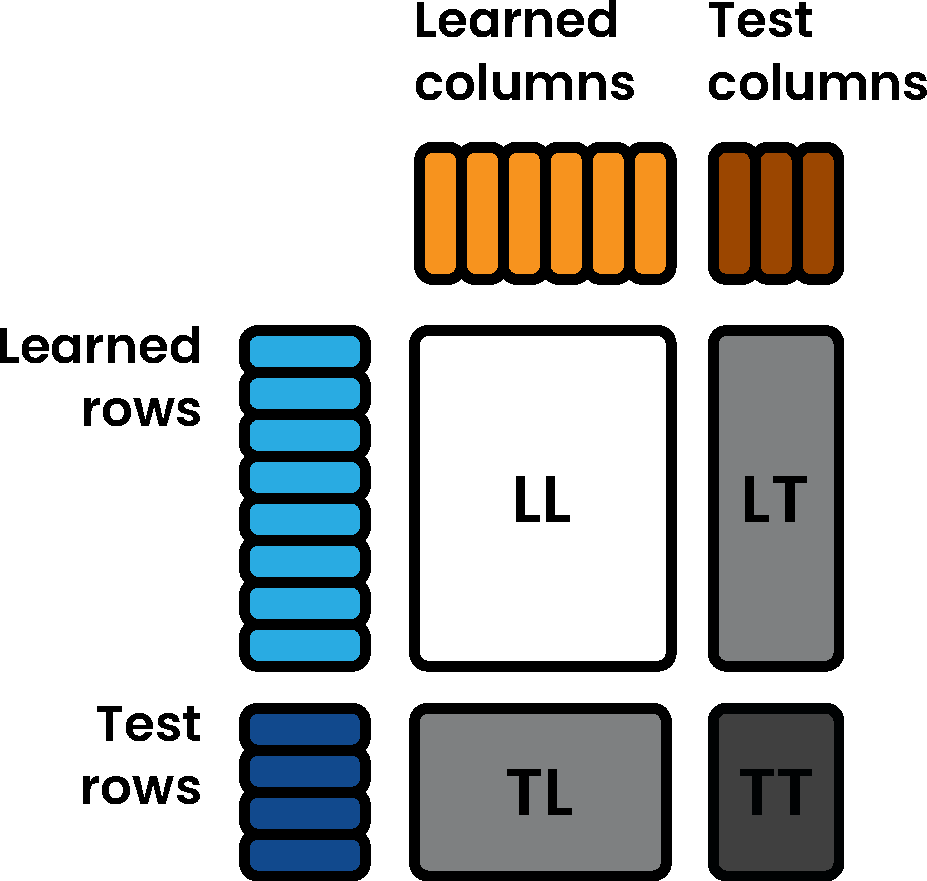
\includegraphics[width=0.4\textwidth]{figures/train_test_split.pdf}
    \caption{Different split configurations for validating models with bipartite datasets.\newline Source: By the author.}
    \label{fig:bipartite test sets}
\end{wrapfigure}

Having two distinct sample groups in bipartite learning settings makes the concept of a held-out set more nuanced. We list five reasonable test configurations we encounter in the literature. Given two samples $\x_1$ and $\x_2$ from each respective domain, a "test set" could refer to:
%
\begin{enumerate}
    \item \textbf{Test $\x_1$, test $\x_2$ (TT):} both $\x_1$ and $\x_2$ are not present in the training set, the model has never seen either of them before;
    \item \textbf{Learned $\x_1$, test $\x_2$ (LT):} $\x_1$ is part of the training feature matrix $X_{1\text{, train}}$, but $\x_2$ was never seen before;
    \item \textbf{Test $\x_1$, learned $\x_2$ (TL):} $\x_2$ is part of the training feature matrix $X_{2\text{, train}}$, but $\x_1$ was never seen before;
    \item \textbf{Learned $\x_1$, learned $\x_2$, masked label (LL-M):}
    Some of the positive annotations in the training set are randomly masked (replacing $1$ by $0$).
    The model is trained on the masked dataset and evaluated based on the predictions for the masked positives and the negative annotations.
    \item \textbf{Learned $\x_1$, learned $\x_2$, unknown label (LL-U):}
    Models trained with the SGSO adaptation (\autoref{sec:standard adaptations}) can exclude specific labels from the training set. All instances are still used for training, but some combinations of them are not presented to the model.
    This corresponds to applying standard validation procedures directly on the $X_\text{SGSO}$ and $Y_\text{SGSO}$ matrices (\autoref{eq:gsodata}).
\end{enumerate}
%
Accordingly, we sometimes call the training set the \emph{LL set}.
LL, TL, LT, and TT were already presented with similar names in previous work~\cite{schrynemackers2015classifying,pliakos2018global,pliakos2020drugtarget}. %TODO other previous paper before schrynemackers2015
The authors call them $L_r \times L_c$, $T_r \times L_c$, and so on.
\cite{pahikkala2015more,ezzat2019computational,liu2016neighborhood} denotes LL-U, LT, TL and TT as S1, S2, S3 and S4, respectively.
\cite{liu2016neighborhood} uses a similar notation, but uses S1 to designate LL-M instead of LL-U. % TODO CHECK
%
The LL-U test set is most frequently used when building SGSO models~\cite{pahikkala2015more}.
%\cite{huang2020moltrans} also reports TL and LT scores.
Using LL-M is more common for matrix factorization methods~\cite{liu2016neighborhood,hao2017predicting,li2019dnilmflda}.

Note that a model that performs well on TT is likely to also perform reasonably well on the other test sets, but the opposite is not necessarily true.
%
For instance, performing well on the TL or LT sets does not mean a model has learned information about both domains. As an example, consider a drug-protein scenario where the model is tested with new drugs and known proteins. Given a specific known protein, a model might correctly infer interactions based on its knowledge that similar drugs have interacted with that protein, or that a specific drug trait correlates well with the protein's interactome. No knowledge about the protein's features is required for the model to make such predictions.
%As a result, this model would be useful to determine which drug characteristics are more important for each protein, but it would be less reliable to understant why the protein selects that drug traits.
Therefore, there is no guarantee that the model will also perform well for new proteins.

Similarly, an effective model according to the LL-U or LL-M settings will not necessarily perform well on any of TT, LT or TL sets. The reason is: an estimator would still be able to perform significantly well on LL-U or LL-M using only the information from the interaction matrix (as matrix factorization algorithms do). There is no guarantee that the model will be a representation of the underlying function: $(\mathbf{x}_1, \mathbf{x}_2) \mapsto y$. As such, there is no guarantee that new instances will be correctly classified, since the only information available about them would be their feature vectors.

On the other hand, the TT test sets are the most informative in terms of generalization. They require the model to fully rely on both input vectors to predict labels, providing a more reliable representation of how attributes from both objects come together to determine the interaction.
%the underlying $(\mathbf{x}_1, \mathbf{x}_2) \mapsto y$.
TT is therefore especially useful when one is interested in gaining insight about the underlying process that generates the interactions. However, they are also the most challenging to predict, and the model's performance on them is expected to be lower than on the other test sets.

In summary, TT should be preferred when the main interest is modeling how input features determine the interaction. TL and LT are useful if generalization is only interesting for one of the domains. LL-U and LL-M are useful when the main goal is to obtain predictions for a defined set of instances, regardless of modeling the function $(\mathbf{x}_1, \mathbf{x}_2) \mapsto y$ or not.

%The TL and LT datasets are useful in more pragmatic scenarios, for example, when searching for a drug molecule to interact with a defined set of targets. In  correctly predicting their interactions is more  

For the learning problems under study, explainability is an important factor to be explored in the future. We thus report our results in terms of TT, LT and TL test sets. Additionally, the learning tasks that we approach represent very diverse phenomena (\autoref{sec:datasets}), which makes the specific LT or TL sets not comparable between datasets. We thus average both LT and TL results together to report a single LT+TL score for each dataset.



%additionally to a traditional "unknown test set" there are two mixed training/test folds possible: we could test our model performance when predicting interactions between instances from $X_1$ that are present in the training set and instances from $X_2$ present in the test set, and vice-versa. Similarly to \ref{pliakos2018}, % TODO: did they invent it?
%we name those settings \emph{LT}, after "learned $X_1$, test $X_2$", and \emph{TL}, after "test $X_1$, learned $X_2$". The usual cross-validation setting with completely new test pairs is then called \emph{TT}, and the training set could alternatively be called the \emph{LL} set.

\subsection{Cross-validating in two dimensions}
\label{sec:cross_validation}

%In the present work, we make use of an adapted $k$-fold cross-validation procedure to evaluate our models' performance. With customary datasets formatted as $X_\text{SGSO}$ and $Y_\text{SGSO}$, $k$-fold cross-validation consists in equally and randomly dividing both $X_\text{SGSO}$ and $Y_\text{SGSO}$ together in $k$ non-overlapping partitions (or folds). The model is then evaluated $k$ times, each time selecting a fold as the test set and the remaining ones as the training set (Figure \ref{}).
In traditional learning tasks, $k$-fold cross-validation consists in equally and randomly dividing both $X$ and $Y$ together in $k$ non-overlapping partitions (or folds). The model is then evaluated $k$ times, in each round selecting a fold as the test set and the remaining ones together as the training set.

In the bipartite interaction setting, fold division can be done in each of the two axis of the interaction matrix, corresponding to each of the two $X_a$ sample domains~\cite{vert2008reconstruction,pahikkala2015more}. Each of the $k_1$ folds of $X_1$ can be combined with one of the $k_2$ folds of $X_2$, resulting in a corresponding partition of $Y$. Each bidimensional fold can be used as the TT set in a CV round, which yields the corresponding four LL, LT, TL and TT sets for each round (\autoref{fig:bipartite diagonal cv}). A $k_1$ by $k_2$ bidimensional CV then has a total of $k_1k_2$ folds.

\begin{figure}[tb]
    \centering
    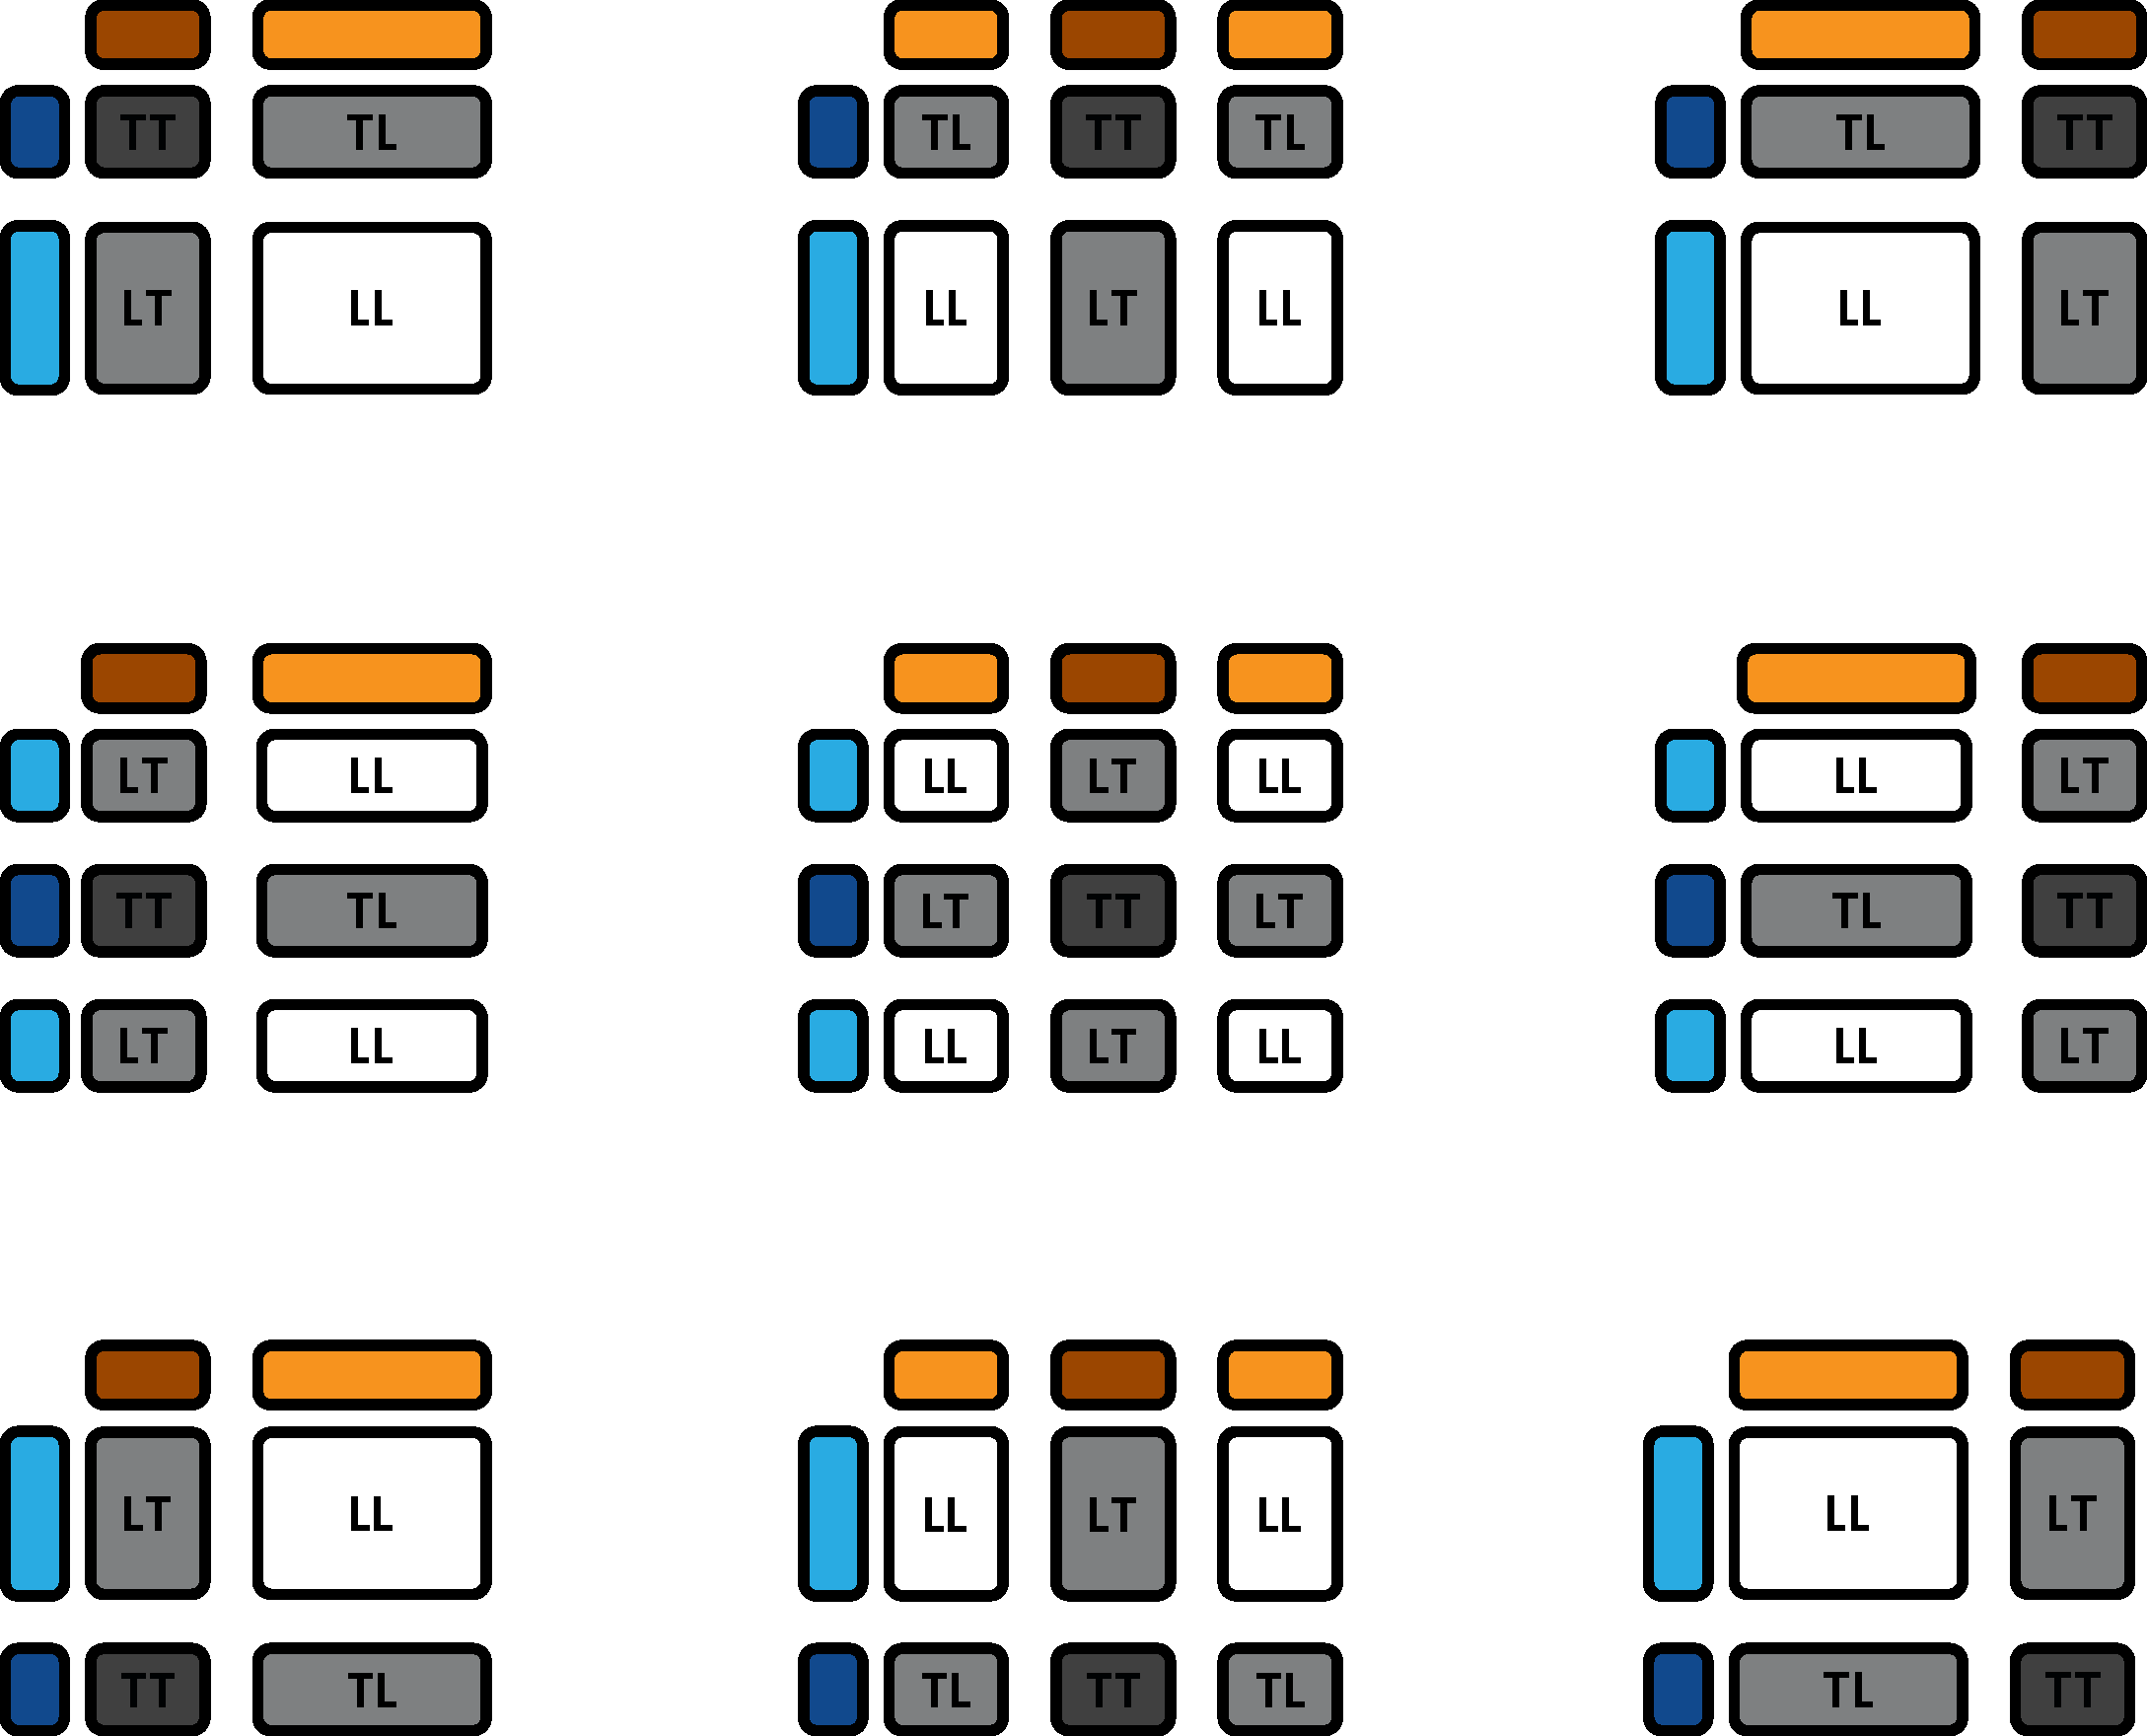
\includegraphics[width=\textwidth]{figures/cv.pdf}
    \caption{Bipartite cross-validation. We represent the 9 train-test splits of a 3 by 3 bipartite cross-validation procedure.\newline Source: By the author.}
    \label{fig:bipartite cv}
\end{figure}

%If all partitions are explored, a $k_1$ by $k_2$ bidimensional cross-validation has a total of $k_1k_2$ folds. 

%However, an argument can be made about not sharing axis-folds between $Y$-folds, to ensure all folds are completely independent and no information is shared between models built on each fold. For instance, if a particular $X_1$ axis-fold happens by chance to be unrepresentative of the remaining instances in $X_1$, all $k_2$ folds that include this axis-fold are expected to yield poor prediction scores. A statistical test comparing two of such score populations then would be biased towards considering those $k_2$ anomalously distributed points as a significant difference, while in reality they come from a single stochastic event, not $k_2$ events as could be apparent.

%To achieve fold-independence, each fold must be built from a completely different pair of axis-folds, which can be simply done by selecting $k=k_1=k_2$ and pairing each $X_1$ axis-fold with a single $X_2$ axis-fold, yielding a total of $k$ folds, not $k^2$ as when all axis-fold combinations are used (Figure \ref{}). While $k_1\neq k_2$ is still theoretically possible, the total number of folds will always be equal to the least $k_a$ value, and the axis corresponding to the greater $k_a$ would have unexploited axis-folds when creating the test sets.

We can optionally enforce independent test sets, so that each dyad composes only one bidimensional fold. This can be done by selecting $k=k_1=k_2$ and pairing each $X_1$ partition with a single $X_2$ partition, yielding a total of $k$ folds, not $k^2$ as before.
%While $k_1\neq k_2$ is still theoretically possible, the total number of folds will always be equal to the least $k_a$ value, and the axis corresponding to the greater $k_a$ would have unexploited axis-folds when creating the test sets.
We refer to this procedure as \emph{diagonal} cross-validation (\autoref{fig:bipartite diagonal cv}).

In our settings, we average the results of all folds of each dataset before computing test statistics. Therefore, the number of folds and the independence between test folds will not affect the final significance estimates. We thus use all $k^2$ folds in our experiments. Diagonal cross-validation is still used, but for the nested validation used for parameter tuning in some experiments.

An important note is that the similarity matrices must be thoughtfully handled when splitting the datasets: we must not include similarities with the test samples in the training set.  % TODO: say that this is usually not addressed?

\begin{figure}[tb]
    \centering
    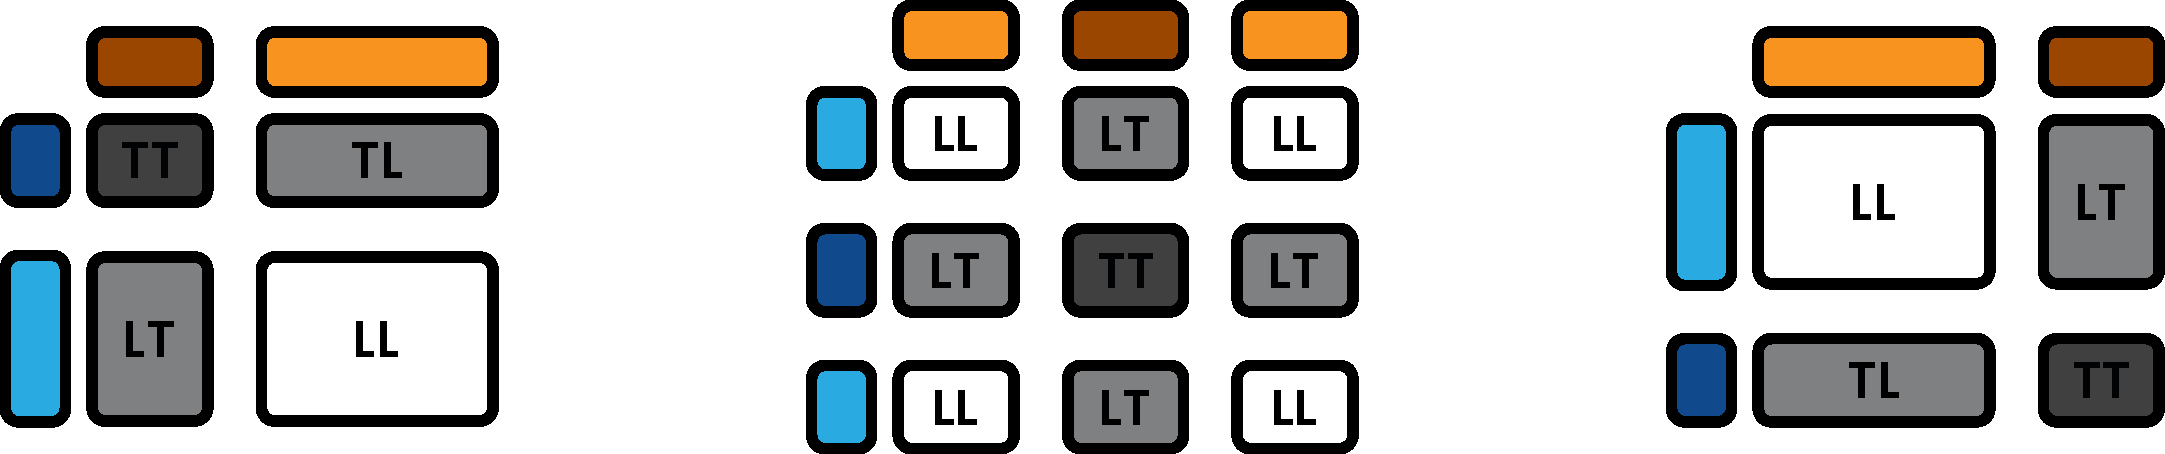
\includegraphics[width=\textwidth]{figures/diagonal_cv.pdf}
    \caption{Diagonal bipartite cross-validation. We represent the 3 train-test splits of a 3 by 3 diagonal bipartite cross-validation procedure.\newline Source: By the author.}
    \label{fig:bipartite diagonal cv}
\end{figure}

%%In order to maximize the amount of training data in each fold, several studies \ref{} perform LT and TL validation separately from the TT validation, employing 1 by $k$ and $k$ by 1 cross-validation procedures respectively for LT and TL settings. Nevertheless, this requires performing cross-validation three times for each estimator, while TT cross-validation already unavoidably generates LT and TL partitions that could be used for scoring. Furthermore, using separate LT, TL and TT validation procedures hinders score comparison between LT and TT and between TL and TT, since different amounts of training data would be used for validating TT in comparison to validating the partially-learned test sets.


\subsection{Prediction scoring metrics}
\label{sec:prediction_metrics}

% TODO classification

This section is concerned with defining the two metrics used throughout this work to evaluate and compare the predictive performance of estimators. The metrics are the \emph{area under the receiver operating characteristic curve} (AUROC) and the \emph{area under the precision-recall curve} (AUPR).
% TODO and explain, justify, etc

Consider a test set of $N$ interaction labels to be inferred by a classifier (we are not concerned with the shape of $Y$ in this section, and $N=|Y|$). Let the classifier's predictions then be represented by a matrix $\hat Y$ of the same shape as $Y$, with $\hat Y\el{ij}$ being the predicted value for the ground-truth label $Y\el{ij}$. Since $Y$ and $\hat Y$ are both binary matrices, there are four possible outcomes when a prediction is made, traditionally quantified~\cite{powers2020evaluation} as follows:
%
\begin{itemize}
    \item \textbf{True Positives (TP):} the number of positive labels correctly predicted, where both the predicted and actual labels are 1.
    \begin{equation}
        TP = \sum_{i,j} \mathbb{I}(Y\el{ij} = 1 \text{ and } \hat{Y}\el{ij} = 1)
    \end{equation}

    \item \textbf{True Negatives (TN):} the number of negative labels correctly predicted, where both the predicted and actual labels are 0.
    \begin{equation}
        TN = \sum_{i,j} \mathbb{I}(Y\el{ij} = 0 \text{ and } \hat{Y}\el{ij} = 0)
    \end{equation}

    \item \textbf{False Positives (FP):} the number of instances where the predicted label is positive (1), but the actual label is negative (0).
    \begin{equation}
        FP = \sum_{i,j} \mathbb{I}(Y\el{ij} = 0 \text{ and } \hat{Y}\el{ij} = 1)
    \end{equation}

    \item \textbf{False Negatives (FN):} the number of instances where the predicted label is negative (0), but the actual label is positive (1).
    \begin{equation}
        FN = \sum_{i,j} \mathbb{I}(Y\el{ij} = 1 \text{ and } \hat{Y}\el{ij} = 0)
    \end{equation}
\end{itemize}
%
where \(\mathbb{I}(A)\) is the indicator function that equals 1 if statement \(A\) is true and 0 otherwise:
%
\begin{equation} % TODO define in general (sec:definitions) or consider always binary
    \mathbb{I} = \begin{cases}
        1 & \text{if } A\\
        0 & \text{otherwise}
    \end{cases}
    \label{eq:indicator}
\end{equation}
%
Notice that the sum of TP, TN, FP and FN is equal to the total number of instances $T$, and we also define $\text{P}=TP+FN$, the total number of \textit{a priori} positive labels in the test set, and $\text{N}=TN+FP$, the total number of \textit{a priori} negative labels. The total number of predicted positives is termed $\text{PP}=TP+FP$ and the remaining predicted negatives are called $\text{PN}=TN+FN$.%TODO cite
%- \(n\) is the total number of instances.
%- \(Y_i\) represents the ground-truth label for instance \(i\).
%- \(\hat{Y}_i\) represents the predicted label for instance \(i\).

% TODO: we use micro version of the metrics. should we use other forms?

Those quantities can be organized in the so-called \emph{confusion matrix}, illustrated by \autoref{fig:scoring}.
%
Naturally, one wants their estimator to maximize TP and TN while minimizing FP and FN.

Most commonly, we do not use these metrics directly, but instead normalize them to the interval [0, 1] in numerous ways. This enables score comparisons across datasets with different numbers of samples and different densities of positive annotations. Below we list the most common normalized scoring metrics for binary classification problems, from which the metrics used in this work are derived~\cite{powers2020evaluation}:
%
\begin{itemize}
    \item \textbf{True positive rate (TPR)} or \textbf{recall:} the ratio of correctly predicted positive labels to the total number of positive labels.
    \begin{equation}
        TPR = \frac{TP}{P} = \frac{TP}{TP + FN}
        \label{eq:tpr}
    \end{equation}
    \item \textbf{True negative rate (TNR):} the ratio of correctly predicted negative labels to the total number of negative labels.
    \begin{equation}
        TNR = \frac{TN}{N} = \frac{TN}{TN + FP}
        \label{eq:tnr}
    \end{equation}
    \item \textbf{False positive rate (FPR):} the ratio of incorrectly predicted positive labels to the total number of negative labels.
    \begin{equation}
        FPR = \frac{FP}{N} = \frac{FP}{FP + TN} = 1-TNR 
        \label{eq:fpr}
    \end{equation}
    \item \textbf{False negative rate (FNR):} the ratio of incorrectly predicted negative labels to the total number of positive labels.
    \begin{equation}
        FNR = \frac{FN}{P} = \frac{FN}{FN + TP} = 1-TPR
        \label{eq:fnr}
    \end{equation}
    \item \textbf{Precision:} the ratio of correctly predicted positive labels to the total number of predicted positive labels.
    \begin{equation}
        Pr = \frac{TP}{PP} = \frac{TP}{TP + FP}
        \label{eq:precision}
    \end{equation}
\end{itemize}
%
These metrics are better visualized in \autoref{fig:scoring}.

An optimal binary classifier will thus present high TPR, TNR and precision while minimizing FPR and FNR.
% TODO note that recall is not affected by PU, point for AUROC

Notice that each of these metrics still allows trivial solutions: if a classifier outputs positive labels for all instances irrespectively of the input features, it will achieve perfect TPR, FNR and Pr, but its TNR and FNR will be null. On the other hand, if a negative label is outputted every time, the opposite will happen.
Thus, we will consider pairs of these metrics simultaneously, such as TPR and TNR.
The selected pair must include at least three of TP, TN, FP, or FN to ensure the whole confusion matrix is taken into account.

Minimizing all the four components of the confusion matrix is not always possible.
%
Most often, the learning algorithms are subject to a tradeoff between the ability to correctly infer positive annotations and the ability to correctly infer negative annotations, that we express as a balance between TPR and TNR. When evaluating models, we must be aware of the relative importances being assigned to each of these tendencies.
%This balance between effective classification of each class is usually formulated as a balance between TPR and TNR.
%
%In real-world scenarios, however, building estimators to simultaneously optimize all these metrics is not a straightforward problem.
%
%In general, classifiers will often lean into one of those directions, displaying a tendency towards yielding more positive
%%(\emph{sensitivity})
%or more negative
%%(\emph{specificity})
%labels.
%
%
This choice is highly application-specific. For instance, in the process of diagnosing medical conditions, TPR is likely to be prioritized, favoring the identification of all true cases at the expense of some misleading positive results.
In this case, the cost of missing a positive result is usually far greater than that of a false positive. In other scenarios such as spam email filtering, TNR might be favored, minimizing the number of legitimate emails marked as spam even if some spam emails go undetected.
%The choice between these tendencies reflects the trade-off between correctly identifying positive instances and correctly identifying negative instances and should align with the specific goals and constraints of the classification problem at hand.

Considering this balance across a variety of learning tasks
is a challenging factor to be taken into account, especially in cases where the estimators can be easily adjusted to favor each class.
%
Many estimators, such as those employed in the present study, do not directly output a binary label but instead provide us with a continuous decision value (such as a probability of interaction) that additionally depends on a threshold parameter to establish the final predicted classes. Formally, the predicted labels $\hat Y$ are obtained from a threshold $t$ applied to the decision values $\tilde Y$:
%
\begin{equation}
    \hat Y\el{ij} = \mathbb{I}(\tilde Y\el{ij} > t)
\end{equation}
%
The selection of $t$ directly affects the propensity to positive or negative outputs, so that a single model can yield multiple different results with varying levels of TPR and TNR depending on the chosen thresholds.
A common practice is then to consider TPR and TNR for all $t$, avoiding the influence of threshold selection on the estimator comparisons.
%Otherwise, the score comparisons could be compromised.

% TODO especially important for our test sets with diffenent density than the training sets
Notice that, since a finite set of outputs is considered for evaluation (the test set), a finite set of thresholds will cover all possible classification results of a model. These results can be easily displayed in a two-dimensional plot, using a point for each considered threshold so that its corresponding TPR and TNR are each indicated by an axis. Conventionally, the TPR is plotted in the $y$ axis while the FPR values (representing the TNR, $FPR=1-TNR$) are presented as $x$ coordinates, which results in the traditional \emph{receiver operating characteristic} (ROC) curve~\cite{davis2006relationship,hand2009measuring,he2009learning,ezzat2019computational}, exemplified by \autoref{fig:roc}.
%
An ideal threshold of an ideal estimator would then be close to the top-left corner of the plot, where TPR and TNR are both 1.
On the other hand, consider a completely random classifier outputting uniformly random values $\hat Y_\text{proba}\el{ij}$ in the 0-1 interval. We would have $\hat Y\el{ij} = \mathbb{I}(\hat Y_\text{proba}\el{ij} > t)$ for a given threshold $t$. This implies that the number of correctly guessed positive labels is $1-t$ (the probability of yielding 1) times the total number of positive labels: $TP = (1-t) (TP+FN)$, which results in $TPR = 1-t$ from the definition. Similarly, $FPR = TPR = 1-t$, so that the ROC curve of a random classifier is a diagonal line from the bottom-left to the top-right corners.

%$FP = (1-t)(TN + FP)$

% TODO interpretation of roc
% TODO its TPR and TNR balance, not TP and TN

To summarize a classifier's performance across all thresholds, the area under the ROC curve (AUROC) is often employed, with values ranging from 0.5 to 1, where 1 represents a perfect classifier and 0.5 represents a random classifier. Although theoretically possible, values below 0.5 would signify the opposite label is being consistently predicted, most likely indicating misconfiguration of the estimator. If AUROC < 0.5, the result can be easily converted to a value greater than 0.5 by simply inverting the predicted labels (turning 0s into 1s and vice-versa).

Despite considerably common, the use of ROC curves requires additional considerations when dealing with heavily imbalanced classification datasets (where some classes are greatly overrepresented)~\cite{he2009learning,saito2015precisionrecall,fernandez2018learning}.
For instance,% let $p$ be the fraction of positive labels relative to the total number of labels: $p = \frac{TP + FN}{N}$.
consider the case where $NEG \gg POS$. Since the denominator of TNR is far greater than the denominator of TPR, a change in TN (for example, missing one more negative label) will have a much smaller impact on TNR than a change in TP (missing a positive label) will have on TPR.
Specifically, an increase of $k$ in TN will cause an increase in TNR $\frac{NEG}{POS}$ times greater than the increase in TPR caused by the same $k$ increase in TP.

% Positive labels (the minority class) have more weight

Given that ROC equally considers both metrics, classifiers that are more sensitive to positive labels will arguably be favored over those prioritizing negative outputs. By the same logic, ROC will also be more lenient towards false positives (that decrease TNR) rather than false negatives (that decrease TPR)~\cite{ozenne2015precision}.

To address this issue, it is commonly suggested the usage of precision-recall (PR) curves instead~\cite{ozenne2015precision,he2009learning,pahikkala2015more,hao2019opensource,ezzat2019computational,yu2020fpscdtia}, where the precision is plotted as the vertical coordinate while the \emph{recall} (another name for TPR) is represented horizontally.
%
The FP term represents the true negatives for a fixed test set (FP = N - TN). Notice that FP in the definition of precision (\autoref{eq:precision}) is not divided by the total number of negative labels, as TN is in TNR. Thus, it is argued that AUPR is less likely than AUROC to prioritize the minority class in imbalanced scenarios~\cite{ozenne2015precision,he2009learning}.

We explore these claims in further detail in the following section, formally defining the ROC and PR curves in terms of ideal label probability distributions.

%In the PR space, considering fixed P and N, a simultaneous increase in TP and TN results in the following improvement in precision:
%%
%\begin{equation}
%    \Delta Pr =
%    \frac{TP + k}{TP + k + FP - k}
%    - \frac{TP}{TP + FP}
%    = \frac{k}{TP + FP}
%    % \frac{k}{TP + FN}
%    % PR area increase: \frac{k^2}{(TP + FP)(TP + FN)}
%    % PR area increase: \frac{k^2}{(TP + FP)(TP + FN)}
%    % PR area increase: \frac{k^2}{(TP + NEG - TN) POS}
%    % ROC area increase: \frac{k^2}{NEG POS}
%\end{equation}
%%
%which is arguably less sensitive to the strategy of increasing FP to obtain larger TP, in comparison with AUROC. %TODO better explanation

% A formal explanation of the differences between ROC and PR curves is developed in the following section.  % TODO: better?
% The following section delves into those considerations with a higher level of detail, formally defining such metrics in the ideal scenario.

% TODO FP represents TN (NEG - TN), so plot TP vs. FP. Precision and recall are similar for those two metrics.

%TODO at least 3 of the 4 basic metrics must be included

% Changes of precision as a function of TN and TP separately
% \begin{equation}
%     \frac{TP}{TP + FP - k}
%     - \frac{TP}{TP + FP}
%     = \frac{TP k}{(TP + FP)(TP + FP - k)}
%     = \frac{TP k}{(TP + FP)^2 - (TP + FP) k}
% \end{equation}
% 
% \begin{equation}
%     \frac{TP + k}{TP + FP + k}
%     - \frac{TP}{TP + FP}
%     = \frac{(TP + k)(TP + FP) - (TP)(TP + FP + k)}{(TP + FP)(TP + FP + k)}
%     = \frac{(TP^2 + TP*FP + kTP + kFP) - (TP^2 + TP*FP + kTP)}{(TP + FP)(TP + FP + k)}
%     = \frac{k FP}{(TP + FP)(TP + FP + k)}
%     = \frac{k (NEG - TN)}{(TP + FP)(TP + FP + k)}
% \end{equation}


% \begin{equation}
%     \sum_t \Delta TPR_t \Delta FPR_t / 2 + TPR_t * FPR_t
%     % = \sum_t \frac{k_t^2}{NEG * POS} / 2 + \frac{TP_t TN_t}{NEG * POS}
%     = \sum_t \frac{k_t^2}{NEG * POS} / 2 + \Delta TNR_t * TPR_t
%     = \sum_t \sum_t \frac{k_t^2}{NEG * POS} / 2
% \end{equation}
% 
% \begin{equation}
%     TPR = tp / pos
%     FPR = fp / (1 - pos)
%     Precision = tp / (tp + fp)
% \end{equation}
% 
% \begin{equation}
%     pos is not the ideal tp + fn, it is simply POS / N
%     you cannot asume c = ppos
% 
%     TPR = (tp/(tp + fp)) * c / pos = prec * c / pos
%     c = pos * TPR (tp + fp) / tp
% 
%     TPR = c - FPR
% 
%     FPR = fp/(fp + tp) * c / (1 - pos)
%     FPR = fp / (fp + tp) * (pos * TPR * (tp + fp)) / ((1 - pos) * tp)
%     FPR = fp * pos * TPR / ((1 - pos) * tp)
%     TPR = ((1 - pos) * tp) * FPR / (pos * fp)
% 
%     Precision = tp / (tp + fp)
%     Precision = 
% \end{equation}
% 
% \begin{equation}
%     TPR = p * c / pos
%     p = pos * TPR / c
%     Precision = p = pos * TPR / c
% \end{equation}

% qualquer estimador é descrito por uma matriz de confusão teórica. Para qualquer estimador, pode se calibá-lo, isso é, usar um parâmetro c que dá uma porcentagem de vezes que, aleatóriamente, mudamos uma predição negativa para positiva ou vice versa. as curvas são em função desse parâmetro. para uma determinada métrica agora em um conjunto de dados real, provemos que o melhor c é o correspondente á proba à priori do conjunto (desbalanceamento). O estimador então pode ajustá-la de acordo com essa proba que ele acha que é a certa. a questão é que ele não tem como saber, então consideramos todas as probas que ele poderia pensar.

% TODO problems with imbalance
% TODO aupr
% TODO problems with imbalance of auroc maybe are not problems with PU learning

%\section{Common approaches to build bipartite models}
%\label{sec:standard adaptations}

\subsubsection{Ideal descriptions of AUROC and AUPRC}
% TODO previous explanations restrained to specific examples and distant analogies. (hans2009 and davis2006 are nice exceptions)

Consider a general estimator outputting a decision value $s \in \mathbb{R}$ for each input instance. The final predicted class $\hat y$ is still to be defined by a threshold $s^*$ so that $\hat y = \mathbb{I}(s > s^*)$. For the ideal case of an infinite number of test samples, the possible scoring results of the estimator would be fully determined by the two theoretical distributions of $s$ given the true label $y$, i.e. the probability density functions $P(s \mid y = 1)$ and $P(s \mid y = 0)$. Similar to \citeonline{hand2009measuring}, we thus define the probability density functions $f_k$ and their corresponding cumulative distribution functions $F_k$ for each of the two classes $k \in \{0, 1\}$:
%
\begin{gather}
    f_0(s) = P(s \mid y = 0) \\
    f_1(s) = P(s \mid y = 1) \\
    F_0(s) = \int_{-\infty}^s f_0(u)\;du \\
    F_1(s) = \int_{-\infty}^s f_1(u)\;du
    \label{eq:ideal_confusion_matrix}
\end{gather}
%
We further define $p=\frac{P}{T}=P(y_\text{test}=1)$ and $n=\frac{N}{T}=P(y_\text{test}=0)$, the fractions of positive and negative labels in the test set, respectively. We can then express the expected values of the confusion matrix as functions of a given threshold $s^*$ for the decision value $s$:
%
\begin{gather}
    \text{TP}(s^*) = p (1 - F_1(s^*)) \\
    \text{TN}(s^*) = n F_0(s^*) \\
    \text{FP}(s^*) = n (1 - F_0(s^*)) \\
    \text{FN}(s^*) = p F_1(s^*)
\end{gather}
%
which, in turn, yields
%
\begin{gather}
    \text{TPR}(s^*) = 1 - F_1(s^*) \\
    \text{TNR}(s^*) = F_0(s^*) \\
    \text{FPR}(s^*) = 1 - F_0(s^*) \\
    \text{FNR}(s^*) = F_1(s^*) \\
    \text{Pr}(s^*) = \frac{p (1 - F_1(s^*))}{p (1 - F_1(s^*)) + n (1 - F_0(s^*))}
\end{gather}

The AUROC can now be expressed as
%
\begin{equation}
    \text{AUROC}
    = \int_{0}^{1} \text{TPR}(\text{FPR}) \;d\text{FPR}
    = \int_{\infty}^{-\infty} \text{TPR}(s) \frac{d\text{FPR}(s)}{ds} \;ds
    = \int_{-\infty}^{\infty} (1 - F_1(s)) f_0(s) \;ds
    \label{eq:auroc0}
\end{equation}
%
The integration limits arise from the fact that FPR is maximal when all instances are classified as positives
%i.e. the decision threshold is as low as possible ($s^* \to -\infty$),
and minimal when all instances are classified as negatives, which respective corresponds to $s^* \to -\infty$ and $s^* \to \infty$. This formulation of AUROC by \autoref{eq:auroc0} leads to the most common intuition behind the metric.
%
The first factor ($1- F(s^*)$), represents the fraction of positive instances that are ranked higher than the threshold $s^*$, alternatively expressed as $\int_{s^*}^{\infty}f_1(s)\; ds$. $f_0$, as defined by \autoref{eq:ideal_confusion_matrix}, represents the probability of finding a negative instance within $s^*$ and $s^* + ds$. Hence, the product of both factors represents the joint probability of having a negative instance between $s^*$ and $s^* + ds$ while also finding a positive instance with $s > s^\ast$. 
%
After integration over all possible thresholds, we conclude that the AUROC score represents the overall probability of randomly selecting a positive instance ranked higher than a randomly selected negative instance.

The baseline score $0.5$ can be derived as follows. A random classifier is defined as an estimator incapable of distinguishing between the true label distributions of each class. That is, a classifier is a random classifier if and only if $f_0(s) = f_1(s) \forall s$. As a consequence,
%
\begin{equation}
    \text{AUROC}
    = \int_{-\infty}^{\infty} (1 - F_0(s)) f_0(s) \;ds
    = -\int_{-\infty}^{\infty} (1 - F_0) \;d(F_0)
    = \left[\frac{(1-F_0)^2}{2}\right]_{-\infty}^{\infty}
    = \frac{1}{2}
    \label{eq:auroc_random}
\end{equation}
 
\autoref{eq:auroc0} also shows a characteristic of AUROC discussed in the previous section: the AUROC score is independent of the relative prevalence of each class in the test set. There is no influence of $p$ or $n$ and only the dependency on the learned decision value distributions.
%it can be desirable to account for this relative importance.
% However, in imbalanced datasets, misclassifying instances of the majority class would  TODO
%
%By definition of the training and test sets, the negative test instances are independent and identically distributed to the negative instances of the training set, with the same being held for the positive instances. Under this assumption, the probability density functions $f_0$ and $f_1$ are independent of the label imbalance of the test set, being solely determined by the nature of the learning algorithm and the training data. As a result, 

% TODO maybe:
%%  We can make this property more clear by expressing AUROC in terms of TN and TP directly (\autoref{eq:auroc_tptn}).
%%  Variations of TP and TN directly represent the number of correctly classified instances of each class, unlike the variation of the decision values $ds$ that is often a more abstract concept.
%%  %While the variation of the decision values $ds$ is a considerably abstract concept in real-world scenarios,
%%  %Variations of TP and TN are directly related to the number of correctly classified instances of each class.
%%  %
%%  \begin{equation}
%%      A_\text{ROC}
%%          = \frac{1}{n} \int_{0}^{n} \frac{\text{TP}(\text{TN})}{p}\;d\text{TN}
%%      \label{eq:auroc_tptn}
%%  \end{equation}
%%  %
%%  %Notice how TP and TN are respectively divided by $p$ and $n$ in \autoref{eq:auroc_tptn}. % TODO better?
%%  From \autoref{eq:auroc_tptn}, the AUROC can \emph{almost} be interpreted as the mean value of TP when TP is expressed in terms of TN, for all TN values. In that case $\frac{1}{n}$ is the normalization factor, the length of the integration interval. This only fact defying that interpretation is the division of TP by $p$. As a result, 
%%  %while TN is simply the integration variable,
%%  TP is weighted by $\frac{p}$, so that smaller values of $p$ attribute more importance to TP relative to TN at each point of the ROC curve.
%  
%  This property, however, can be seen as a disadvantage in imbalanced datasets.
%  


% NOTE: I don't think so.
%  This property precisely defines the specific implications of using AUROC for imbalanced datasets presented by \autoref{sec:evaluation_protocol}. In such cases, one must have in mind that misclassifications will effectively be inversely weighted by their respective true class prevalences, with misclassifications of the majority class being more tolerated individually than those of the minority class. In other words, AUROC will be more lenient towards false positives than false negatives if positives are the underrepresented class of a problem.
%  %TODO for an estimator with same TP and TN but different p and n, ...
%  %TODO variational calculus, how to hack the auroc
%  %TODO aucroc is proportional to the expected accuracy
%  
%  If the class distribution of the test set is not an inherent property of the problem under study and the main research interest lies in probing the underlying label distributions $f_0$ and $f_1$, this independence from $p$ may be a desired characteristic of AUROC. However, if the label imbalance is in fact a consistent feature of the learning task, taking it into consideration may report a more realistic portrait of the model performance in future studies. If the positive class is always heavily underrepresented in a given learning task, for example, one may intend to prioritize the correct classification of negative instances, since the overall number of correct classifications will be more influenced by them. More generally, the choice to be made is usually between scoring based on the absolute metrics TP and TN, directly related to the number of samples, or the relative metrics TPR and TNR, relying on fractions of negatives and positives.
%  
%  In scenarios of high class imbalance and where the absolute metrics are the main focus,
%  % TODO maybe remove following
%  i.e. constraining the number of false positives is as important as increasing the number of true positives,
%  it is often recommended the usage of precision-recall (PR) curves as a replacement for ROC~\cite{ozenne2015precision,he2009learning,krawczyk2016learning,fernandez2018learning}.
%  %TODO the precision weights fp as blablabl
%  %XXX

The AUPR is defined as
%
\begin{multline}
    \text{AUPR}
    = \int_{0}^{1} \text{Pr}(\text{TPR}) \;d\text{TPR}
    = \int_{\infty}^{-\infty} \text{Pr}(s) \frac{d\text{TPR}(s)}{ds} \;ds
    =\\
    = \int_{-\infty}^{\infty} \text{Pr}(s) f_1(s)\;ds
    = \int_{-\infty}^{\infty} \frac{p (1 - F_1(s)) f_1(s) \;ds}{p (1 - F_1(s)) + n (1 - F_0(s))}
    \label{eq:auprc0}
\end{multline}
%
From \autoref{eq:auprc0}, AUPRC can be interpreted as the average precision weighted by the distribution of positive instances. Analogously, it corresponds to collecting the decision values attributed to each positive instance, and then calculating the average precision considering only these values as classification thresholds.
Furthermore, unlike AUROC, the true label cumulative distributions ($F_0$ and $F_1$) appear each weighted by their respective class prevalences ($p$ and $n$).
%Here it may be useful to bring back the discrete scenario of real classification problems, where each sample of the training set defines a threshold $s*$. With the precision weighted by the positive samples' distribution in \autoref{eq:auprc0}, AUPRC would thus be the average precision considering only the threshold values $s*$ defined by a true positive sample.

% TODO maybe:
%% Furthermore, the true label cumulative distributions ($F_0$ and $F_1$) appear each weighted by their respective class prevalences ($p$ and $n$). As a result, expressing the AUPR in terms of TP and FP yields no dependence on $p$ or $n$ apart from dividing by the length of integration interval $\frac{1}{p}$ that characterizes the averaging procedure:
%% %
%% \begin{equation}
%%     A_\text{PRC}
%%     =
%%         \frac{1}{p}
%%         \int_{0}^{p}
%%             \left(1-\frac{\text{FP}}{\text{TP}}\right)^{-1}
%%         \;d\text{TP}
%%     % =
%%     %     \frac{1}{p}
%%     %     \int_{0}^{p}
%%     %         \left(1-\frac{n-\text{TN}}{\text{TP}}\right)^{-1}
%%     %     \;d\text{TP}
%% \end{equation}
%
% TODO why FP instead of TN write in the previous section
% Another distinguishing characteristic of AUPR is its dependence on FP rather than TN.


\subsubsection{AUPR and AUROC in terms of ranked decision values}
\label{sec:metrics from ranks}

%To better describe the differences between using the absolute metrics and the relative metrics, we can once again bring our theoretical formulation closer to real-world applications.
When computing AUROC or AUPR for a given estimator on a test set, the values of the decision function $s$ are usually not directly considered. Instead, the decision values outputted for each test instance are used to rank them from lowest to highest, and from these ranked test labels the curves and respective areas are obtained. The specific values of $s$ are thus indifferent to the scoring process, as long as the ranking is preserved. If the percentile rank of each test instance is denoted by $r \in [0, 1]$ and each test instance is associated with a decision value, there is a one-to-one monotonic correspondence between $r$ and $s$ in the limit of an infinite number of test samples.
% While $s$ can often represent a rather abstract concept, $r$ is directly related to the number of instances below a given threshold.
Formally, we have
% TODO we take the freedom to represent f(r) = f(s(r))
%
%\begin{equation}
%    f(s) = P(s) = pf_1(s) + nf_0(s)
%\end{equation}
%
\begin{gather}
    r(s) = pF_1(s) + nF_0(s)\\
    dr = [pf_1(s) + nf_0(s)] \; ds
\end{gather}

We also take the liberty to represent $g(r) = g(s(r))$, so that
%Therefore, %$\frac{d F_1(r)}{dr} = \frac{f_1(r)}{pf_1(s) + nf_0(s)}$.
\begin{gather}
    F_1(r) = \int_0^r \frac{f_1(r)}{pf_1(r) + nf_0(r)} \; dr\\
    \frac{d F_1(r)}{dr} = \frac{f_1(r)}{pf_1(r) + nf_0(r)}
\end{gather}
%
%so that a change $dr$ represents a change in the number of instances between $s$ and $s+ds$. 
AUPR as defined in \autoref{eq:auprc0} can now be written as
%
\begin{multline}
    \text{AUPR}
    = p \int_{0}^{1}
        %\frac{1 - \int \frac{f_1(r)}{f(r)} \;dr}{(p+n) - [pF_1(r) + nF_0(r)]}
        \frac{1 - F_1(r)}{(p+n) - [pF_1(r) + nF_0(r)]}
        \; \frac{f_1(r)}{[pf_1(s) + nf_0(s)]}
    \;dr
    =\\
    = p \int_{0}^{1}
        \frac{[1 - F_1(r)]}{[1 - r]}\frac{d F_1(r)}{dr}
    \;dr
    %=\\
    = -\frac{p}{2} \int_{0}^{1}
        \frac{1}{1 - r}
        \; \frac{d [1 - F_1(r)]^2}{dr}
    \;dr
    =\\
    =
    - \frac{p}{2}
    \left|
        \frac{[1 - F_1(r)]^2}{1 - r}
    \right|_0^1
    + \frac{p}{2}
    \int_{0}^{1}
        \left[\frac{1 - F_1(r)}{1 - r}\right]^2
    dr
    % =
    % \frac{p}{2} \left\{
    %     1 - \lim_{r \to 1} \frac{[1 - F_1(r)]^2}{1 - r}
    %     + \int_{0}^{1}
    %         \left[\frac{1 - F_1(r)}{1 - r}\right]^2
    %     dr
    % \right\}
    =\\
    =
    \frac{p}{2}
    \left\{
        1 + \int_0^1 \left[\frac{1 - F_1(r)}{1 - r}\right]^2 dr
    \right\}
    =
    \frac{p}{2}
    \left\{
        1 + \int_0^1 [\text{Pr}(r)]^2 dr
    \right\}
    \label{eq:aupr ranks}
\end{multline}
%
% where we define
% %
% \begin{gather}
%     c(r) = \frac{p f_1(r)}{f(r)} = \frac{p f_1(r)}{pf_1(r) + nf_0(r)}\\
%     C(r) = \int c(r) \;dr = p F_1(r)
% \end{gather}
%
% \begin{multline}
%     \int_{0}^{1}
%         \frac{1 - \frac{1}{p}C(r)}{1 - r}
%         \; c(r)
%     \;dr
%     = \int_{0}^{1}
%         \frac{1}{1 - r}
%         \; \left(-\frac{p}{2}\right)
%         \; \frac{d [1 - \frac{1}{p}C(r)]^2}{dr}
%     \;dr
%     =\\
%     =
%     - \frac{p}{2}
%     \left|
%         \frac{[1 - \frac{1}{p}C(r)]^2}{1 - r}
%     \right|_0^1
%     + \frac{p}{2}
%     \int_{0}^{1}
%         \left[\frac{1 - \frac{1}{p}C(r)}{1 - r}\right]^2
%     dr
%     % =
%     % \frac{p}{2} \left\{
%     %     1 - \lim_{r \to 1} \frac{[1 - \frac{1}{p}C(r)]^2}{1 - r}
%     %     + \int_{0}^{1}
%     %         \left[\frac{1 - \frac{1}{p}C(r)}{1 - r}\right]^2
%     %     dr
%     % \right\}
%     =\\
%     =
%     \frac{p}{2}
%     \left\{
%         1 + \int_0^1 \left[\frac{1 - F_1(r)}{1 - r}\right]^2 dr
%     \right\}
%     \label{eq:auprc2}
% \end{multline}
%
in which the upper boundary term is determined by using L'Hôpital's rule and noticing that $F_1(r=1) = 1$ and
%$\frac{d F_1(r)}{dr} = \frac{f_1(r)}{pf_1(r) + n f_0(r)} \le \frac{1}{p}$.
$\frac{d F_1(r)}{dr} \le \frac{1}{p}$.
%
\begin{equation*}
    \lim_{r \to 1} \frac{[1 - F_1(r)]^2}{1 - r}
    %= \lim_{r \to 1} \frac{- 2 [1 - F_1(r)] c(r)}{- p}
    = 2 \cdot \lim_{r \to 1} \left[1 - F_1(r)\right] \frac{d F_1(r)}{dr}
    % = (2)\lim_{r \to 1} (1 - 1) \frac{d F_1(r)}{dr}
    = 0
\end{equation*}
%
\autoref{eq:aupr ranks} reveals that AUPR is closely related to the average squared precision across all ranks.
%\autoref{eq:auprc2} shows us that AUPRC, when expressed in terms of percentile rankings, has a simple linear dependency on the positive class prevalence $p$ of the test set. Although not completely independent, this simple relationship makes the comparison of AUPRC scores across test sets with different class distributions a straightforward task. % TODO predictable well-behaved Just a matter of rescaling.

%Another consequence of \autoref{eq:auprc2} is a new interpretation of AUPRC as a linear function over the average \emph{squared} precision across all possible thresholds.

% TODO auroc becomes interesting again for PU

%  The same does not hold for the area under the ROC curve. 
%  
%  % TODO:
%  Consider the ranking of a binary classification test set produced by a given classifier (\autoref{}). Green dots represent positive labels while red dots represent negative labels. A threshold is still to be defined, so the only output of the classifier is the order of test instances represented in the figure, indicating which instances the classifier believes are more likely to belong to the positive class (instances to the right are thought to have higher probability to be positive than instances to the left). Splitting the produced ranking in several equally-sized windows, we call $c\el i$ the average fraction of positive labels in the $i$-th window:
%  %
%  \begin{equation}
%      c \el i = \frac{\text{# of positives in window }i}{\text{window length}\times \text{P}}
%  \end{equation}

%%% TODO: c(r) has a maximum value of 1/p, but it shouldn't depend on p?
%%For a sufficiently large number of samples, $c\el i$ approximates a function $c(r)$ describing the density of positive labels as a function of the classifier's percentile ranking $r$. The probability of classifying a sample between $r$ and $r+dr$ as positive is then given by $c(r)dr$, while $\int_{0}^{1}c(r)\;dr = 1$. Notice that $c(r)$ is independent of the label imbalance of the test set, since it is normalized by the fraction of positive labels $P$ and depends only on the underlying probabilities of predicting a decision value given the true label. For instance, consider a classifier characterized by the distributions% as suggested by \citeonline{saito2015precisionrecall}:
%%%
%%\begin{gather}
%%    P(\hat Y\el{ij} = 1 | Y\el{ij} = 1) = \beta(1, 4) \\
%%    P(\hat Y\el{ij} = 1 | Y\el{ij} = 0) = \beta(4, 1)
%%\end{gather}
%%%
%%$c(r)$ will be given by
%%%
%%\begin{equation}
%%    c(r) = P(\hat Y\el{ij} = 1 | r) = \frac{\beta(1, 4)}{\beta(4, 1) + \beta(1, 4)}
%%\end{equation}
%%%
%%as illustrated by \autoref{fig:}.
%%
%%% TODO define confusion matrix
%%Plotting $p \cdot c(r)$ as a function of the percentile ranking offers an interesting way of visualizing the confusion matrix generated by each threshold, since the threshold values naturally have a one-to-one monotonic relationship with the values of $r$ (\autoref{fig:}). Under this representation, we can define
%%%
%%\begin{equation}
%%    tp(r) = \frac{TP}{N} = p\left(1 - \int_{0}^{r} c(r)\;dr\right)
%%\end{equation}
%%\begin{equation}
%%    tn(r) = \frac{TN}{N} = r - p\int_{0}^{r} c(r)\;dr
%%\end{equation}
%%\begin{equation}
%%    fp(r) = \frac{FP}{N} = n - r + p\int_{0}^{r} c(r)\;dr
%%\end{equation}
%%\begin{equation}
%%    fn(r) = \frac{FN}{N} = p\int_{0}^{r} c(r)\;dr
%%\end{equation}
%%%
%%which yields
%%%
%%\begin{equation}
%%    tpr(r) = \frac{tp(r)}{p} = 1 - \int c(r)\;dr
%%\end{equation}
%%\begin{equation}
%%    fpr(r) = \frac{fp(r)}{n} = 1 - \frac{r}{n} + \frac{p}{n}\int c(r)\;dr
%%\end{equation}
%%\begin{equation}
%%    pr(r) = \frac{tp(r)}{1-r} = \frac{p}{1-r} \left(1 - \int c(r)\;dr\right)
%%\end{equation}
%%%
%%As such, the area under the ROC curve (AUROC) is now given by
%%%
%%\begin{multline}
%%    A_\text{ROC}
%%    = \int_{0}^{1} tpr \;d(fpr)
%%    = -\int_{fpr(1)}^{fpr(0)} tpr \frac{d(fpr)}{dr} \;dr
%%    %= \int_{1}^{0} \left(1 - \int c(r)\;dr \right) \frac{1}{n} \left(-1 + p\,c(r)\right) \;dr
%%    =\\
%%    = \int_{0}^{1} \left(1 - \int c(r)\;dr \right) \frac{1}{n} \left(1 - p\,c(r)\right) \;dr
%%    \label{eq:auroc1}
%%\end{multline}
%%%
%%\autoref{eq:auroc1} leads to the most commonly promoted intuition behind AUROC. Notice that the analogous of the function $c(r)$ for the negative class can be found with 
%%$\frac{1}{n} \left(1 - p\,c(r)\right)$, precisely the last factors of \autoref{eq:auroc1}.
%%%
%%The first factor ($1- \int c(r)\;dr $), on the other hand, represents the fraction of positive instances that are ranked higher than the threshold $r$.
%%%
%%As a consequence, both factors combined represent the probability of finding a negative instance between $r$ and $dr$ while also finding a positive instance with a higher rank than that of the negative instance.
%%%
%%Upon integration over all possible thresholds, we conclude that the AUC ROC score represents the overall probability of randomly selecting a positive instance ranked higher than a randomly selected negative instance.

We can also express the AUROC in terms of the percentile ranks:
%
\begin{multline*}
    \text{AUROC}
    = \frac{1}{n} \int_{0}^{1}
        (1 - F_1(r)) \left(\frac{n f_0(r)}{nf_0(r) + pf_1(r)}\right) \;dr
    =\\
    =  \frac{p}{n} \int_{0}^{1}
        (1 - F_1(r)) \left(1 - \frac{pf_1(r)}{nf_0(r) + pf_1(r)}\right) \;dr
    =\\
        = \frac{1}{n} \int_{0}^{1} (1 - F_1(r)) \left(1 - p \frac{dF_1(r)}{dr}\right) \;dr
    =\\
    =
        \frac{1}{n} \int_{0}^{1} (1 - F_1(r)) \;dr
        - \frac{p}{n} \int_{0}^{1}
            (1 - F_1(r)) \;d(F_1(r))
    =\\
    =
        \frac{1}{n} \int_{0}^{1} (1 - F_1(r)) \;dr
        + \frac{p}{n} \left[
            \frac{(1 - F_1(r))^2}{2}
        \right]^1_0
    =\\
    =
        \frac{1}{n} \left\{
            \int_{0}^{1} (1 - F_1(r)) \;dr - \frac{p}{2}
        \right\}
    \label{eq:auroc ranks}
\end{multline*}

Equations \ref{eq:aupr ranks} and \ref{eq:auroc ranks} put AUPR and AUROC in a similar format, better delineating the differences between the two metrics. Consider expressing both now in terms of the precision.
%
\begin{gather}
    \text{AUROC} = \frac{1}{n} \left\{
        \frac{1}{p}\int_{0}^{1} (1 - r)\text{Pr}(r) \;dr - \frac{p}{2}
    \right\}\\
    \text{AUPR} = \frac{1}{2} \left\{
        p + \frac{1}{p}\int_0^1 \text{Pr}(r)^2 dr
    \right\}
\end{gather}
%
%\begin{gather}
%    A_\text{ROC} = \frac{1}{n} \left\{
%        \int_{0}^{1} (1 - F_1(r)) \;dr - \frac{p}{2}
%    \right\}\\
%    A_\text{PR} = \frac{p}{2} \left\{
%        1 + \int_0^1 \left[\frac{1 - F_1(r)}{1 - r}\right]^2 dr
%    \right\}
%\end{gather}
%
%\begin{gather}
%    A_\text{ROC} = \frac{1}{n} \left\{
%        \int_{0}^{1} \text{TPR}(r) \;dr - \frac{p}{2}
%    \right\}\\
%    A_\text{PR} = \frac{p}{2} \left\{
%        1 + \int_0^1 \left[\frac{\text{TPR}(r)}{1 - r}\right]^2 dr
%    \right\}
%\end{gather}

% As a function of F_0:
%
% \begin{gather}
%     A_\text{PR}
%     = \frac{p}{2} \left\{
%         1 + \int_0^1 \left[\frac{\text{TPR}(r)}{1 - r}\right]^2 dr
%     \right\}
%     =\\
%     = \frac{1}{2} \left\{
%         p + \frac{1}{p}\int_0^1 \left[\frac{p - pF_1(r)}{1 - r}\right]^2 dr
%     \right\}
%     = \frac{1}{2} \left\{
%         p + \frac{1}{p}\int_0^1 \left[\frac{p - r + nF_0(r)}{1 - r}\right]^2 dr
%     \right\}
%     =\\
%     = \frac{1}{2} \left\{
%         p + \frac{1}{p}\int_0^1 \left[\frac{1 - r - n(1 - F_0(r))}{1 - r}\right]^2 dr
%     \right\}
%     =\\
%     = \frac{1}{2} \left\{
%         p + \frac{1}{p}\int_0^1 \left[1 - \frac{n(1 - F_0(r))}{1 - r}\right]^2 dr
%     \right\}
% \end{gather}
%
% Using precision, also interesting:
%
%
%Ignoring constant terms and factors, both metrics are centered on integrating the TPR over all possible ranks, each rank representing a classification threshold. The crucial difference is that AUROC equally considers all TPR values, while AUPR weights each TPR value by the inverse of the reversed ranks.
Ignoring constant terms and factors, both metrics are centered on integrating the precision over all possible ranks, each rank representing a classification threshold. The crucial difference is that AUPR equally considers all precision values, while AUROC weights each $\text{Pr}(r)$ value by the the reversed ranks.

%Notice that $\text{Pr}(r^\ast)$ for a given $r^\ast$ sums $f_1(r)$ over all $r > r^\ast$ values, only considering the ranks higher than $r^\ast$. As a result, the $r$ values closer to $1$ will have a larger influence when integrating over the precisions (a sum of sums of $f_1$), since $r\approx 1$ will be considered for a larger number of terms.

The precision metric is normalized by the number of instances it considers, so precision values in different $r$ have comparable magnitude.
%
With this in mind, notice that the precision values calculated for $r\approx 1$ are obtained from a very small number of labeled instances. As a result, each label considered when $r \approx 1$ has a large influence on the $Pr(r)$ value, and precisions will tend to have larger variances when $r\approx 1$.
%
Therefore, the AUPR metric is more influenced by the label value of the highest ranked instances, since it equally considers all precision values.

Additionally, the quadratic exponent of AUPR's integrand emphasizes higher precision values overall, independently of the number of samples on which they were calculated ($1 - r$). This would amplify the effect of high $Pr(r)$ values for $r \approx 1$ resulting from stochastic label variations.
Hence, we suggest that the AUPR metric is more prone to noise in the labels of higly ranked samples, prioritizing models that strictly maintain high precision for a smaller selection of highest ranks.

%Notice that the TPR reduces as $r$ is increased (\autoref{eq:}). Therefore, equally considering all TPR values in the integration interval naturally prioritizes ranks that are closer to 0.
%TODO:
%Another formulation is possible by expressing AUROC in terms of the precision. When $r$ is closer to $0$, $Pr(r)$ is calculated over a larger number of samples, so that . AUROC emphasizes the precision values
%
%On the other hand, AUPR compensates this effect, dividing each TPR value by $1 - r$. 
%At first sight, one could think that this would lead to considering all ranks on a mo
%
%Each TPR(r) thus will have the same weight on the score regardless of $r$.
%  In this case, notice that the precision values calculated for $r\approx 1$ are obtained from a very small number of labeled instances. As a result, the $Pr(r)$ values for $r\approx 1$ will tend to have larger variances.
%  Furthermore, the quadratic exponent of AUPR's integrand emphasizes higher precision values overall, independently of the number os samples on which they were calculated. This would amplify the effect of high $Pr(r)$ values for $r \approx 1$, that could be primarily resulting from stochastic variations.
%  Therefore, we hypothesize that the AUPR metric is more prone to stochastic variations in the labels of higly ranked samples, prioritizing models that strictcly maintain high precision for a smaller selection of higher ranks.
% Even though they receive the same weight as the TPR values for larger $r$.
%
%
%Therefore, the AUPR metric emphasizes the effect of the highest ranked instances. 
%
%Additionally, the square exponent in AUPR's integrand further prioritizes high values of $\frac{\text{TPR}(r)}{1-r}$, likely reinforcing the effect.
%
% In other words, AUPR's penalty for having false negatives is much higher when the rank is also high ($\text{TPR} = 1 - \text{FNR}$).
%
% Keeping the same number of selected instances, FPR = PPOS - TPR
% Therefore, AUPR tends to ensure that the highest ranked instances are indeed true positives,
%On the other side, AUROC is more concerned with precision values calculated for higher ranks, being more likely to allow some highly-ranked false positives.
On the other side, AUROC compensates this effect by weighting each $\text{Pr}(r)$ value by $1 - r$, so that precision values calculated for lower ranks are prioritized. The prioritized precision values ($r\approx 0$) are calculated from a larger number of labels, having lower variances and being more robust to label noise. Each label considered when $r \approx 0$ has a smaller influence on the $Pr(r)$ value relative to the other labels being considered. However, AUROC assigns a larger weight to these precision values, so the influence of smaller ranks also tend to increase.

%is more concerned with precision values calculated for higher ranks, being more likely to allow some highly-ranked false positives.
%This effect is more pronounced if only a few positive annotations are present in the test set, since it is probabilistic easier to achieve higher TPR values for 

% MOVED TO RESULTS
%Overall, using AUPR is more suited when one is interested in selecting a restricted number of top-ranked instances from a pool of predictions, such as in recommendation systems or drug discovery tasks.
%Conversely, AUROC should be favored when the goal is to rank a large batch of interactions. Examples would be modeling genetic interactions in a genome-wide fashion or building interaction databases.
%
%We also argue that AUROC could be preferable for comparing models under the PU assumption, at least in purely theoretical settings. For PU datasets, we naturally expect some negative-labeled instances to be very highly ranked since they could be, in fact, unannotated positives. AUPR would more strictly penalize such predictions, favoring models that consider the labeling mechanism itself rather than only the underlying interaction mechanism. AUPR could thus undermine the model's potential to discover new interactions, likely failing to gauge the generalization capabilities of algorithms in a PU context.
%
%
%%AUPR, for instance, could emphasize a model that simply predicts higher probabilities for more frequently interacting samples
%
%Conversely, the importance of AUPR lies in applied scenarios where selecting false positives could be costly or have significant negative impacts. For instance, when selecting a small number of drug candidates for further testing.

%Even in this scenario, if one has beforehand the number $k$ of candidates to be selected, one could consider $k$ when building new estimators for the task. For instance, using the precision on the best $k$ probabilities could be more informative than the AUPR or AUROC scores, ensuring that the same importance is given to all the $k$ candidates.  % TODO: this is not a good idea, too volatile and failing to generalize

This characteristic of AUROC might be more suitable for model comparison under the ositive-unlabeled assumption, even though AUPR is usually reccomended for imbalanced scenarios~\cite{he2009learning,saito2015precisionrecall,fernandez2018learning}.
In PU datasets, it is common for negative-labeled instances to rank highly due to the possibility of them being unannotated positives. These highly-ranked negatives would have a larger influence on the AUPR score in comparison to the AUROC score.
In fact, we show in the next section that AUROC is closely related to the Mean Percentile Rank metric, which has been suggested for PU learning contexts of interaction prediction and recommendation systems~\cite{pahikkala2015more,johnson2014logistic,hao2019opensource,yu2020fpscdtia}. \autoref{sec:comparing auroc aupr} presents further discussion on the specific usecases of AUPR and AUROC, besides a numerical analysis of their dependence on the percentile ranks.


% TODO indeed the results tend to change less with AUROC across ILR in comparison to AUPR
% TODO which metric is better for PU
% TODO what are the differences in each metric
% if we have the number of prediction, eavluate it


\subsubsection{AUROC is the normalized mean percentile ranks}
\label{sec:auroc mpr}

From \autoref{eq:auroc ranks}, we can express AUROC as
% Defining $C(r) = \int c(r) \; dr$, we can write
%
\begin{multline}
    \text{AUROC}
        = \frac{1}{n} \left\{
            \int_{0}^{1} (1 - F_1(r)) \;dr - \frac{p}{2}
        \right\}
    =\\
        = \frac{1}{n} \left\{
            1 - \int_{0}^{1} F_1(r) \;dr - \frac{p}{2}
        \right\}
    %=\\
        = \frac{1}{n} \left\{
            1 - \int_{0}^{1} \frac{d(r)}{dr}F_1(r) \;dr - \frac{p}{2}
        \right\}
    =\\
        = \frac{1}{n} \left\{
            1 - \left[rF_1(r)\right]_0^1 + \int_{0}^{1} r \frac{d F_1(r)}{dr} \;dr - \frac{p}{2}
        \right\}
    %=\\
        = \frac{1}{n} \left[
            \int_{0}^{1} r \;d F_1 - \frac{p}{2}
            %\int_{0}^{1} r \frac{d F_1(r)}{dr} \;dr - \frac{p}{2}
            %\int_{0}^{1} r \tilde f_1 \;dr - \frac{p}{2}
        \right]
    \label{eq:auroc mpr}
\end{multline}
%
\autoref{eq:auroc mpr} offers another perspective on AUROC. The term $\int_{0}^{1} r\,d F_1(r)$ represents the expected percentile rank of the positive samples:
%
\begin{equation}
    \int_{0}^{1} r\,d F_1(r) = E[r \mid y = 1] = \text{MPR}
    \label{eq:mpr}    
\end{equation}
%
% TODO XXX moment of inertia
% TODO roc is again interesting for PU data, MPR
%
%The term $\int_{0}^{1} r\,c(r) \;dr$ represents the average percentile ranking of positive labels, or the average distance of a positive label from the origin in the plot of $c(r)$. This quantity by itself, the mean percentile ranking (MPR), is a common metric in the realm of collaborative filtering for recommendation systems~\cite{hu2008collaborative,johnson2014logistic} and has also been proposed to bipartite interaction prediction~\cite{ezzat2019computational,hao2019opensource,yu2020fpscdti}.
%or the average distance of a positive label from the origin in the plot of $c(r)$.
This quantity is sometimes referred to as the \emph{mean percentile ranking} (MPR) in the previous literature~\cite{johnson2014logistic}, being proposed in contexts of recommendation systems~\cite{hu2008collaborative,johnson2014logistic} and bipartite interaction prediction~\cite{ezzat2019computational,hao2019opensource,yu2020fpscdtia}.
%
%\begin{equation}
%    \text{MPR} = \int_0^1 r\,c(r) \;dr
%\end{equation}
%
%At first glance, MPR seems to offer some advantages over AUROC: besides simpler in formulation, MPR also seemingly does not depend on $p$ or $n$, the relative amounts of postive and negative labels in the test set, making comparisons across different test sets more direct. However, consider the maximum and minimum values of MPR, achieved for the ideal $c(r)$ distributions:
%

Consider now the maximum and minimum values of MPR, achieved, respectively, for the ideal $f_1(r)$ distributions:
%
\begin{gather}
    f_{1, \text{max}}(r) = \frac{1}{p}\mathbb{I}(r > n)\\
    f_{0, \text{max}}(r) = \frac{1}{n}\mathbb{I}(r < n)\\
    f_{1, \text{min}}(r) = \frac{1}{p}\mathbb{I}(r < p)\\
    f_{0, \text{min}}(r) = \frac{1}{n}\mathbb{I}(r > p)
\end{gather}
%
Applying these definitions to determine $\frac{dF_1(r)}{dr}$ and using the results in \autoref{eq:mpr}, we obtain
%
%%\begin{gather}
%%    \frac{d F_1(r)}{dr} = \frac{f_1(r)}{pf_1(r) + nf_0(r)} \le \frac{1}{p}\\
%%\end{gather}
%
%\begin{gather}
%    c_\text{max}(r) = \frac{\mathbb{I}(r > n)}{p}\\
%    c_\text{min}(r) = \frac{\mathbb{I}(r < p)}{p}
%\end{gather}
%
% The extrema of MPR do in fact depend on $n$:
% %
% \begin{equation}
%     \text{MPR}_\text{max}
%         = \int_(1-p)^1 r\;dr
%         = \frac{1 - n^2}{2p}
%         = \frac{1 + n}{2}
% \end{equation}
% %
% \begin{equation}
%     \text{MPR}_\text{min}
%         = \frac{1}{p}\int_0^p r \;dr
%         = \frac{p^2}{2p}
%         = \frac{p}{2}
%         = \frac{1 - n}{2}
% \end{equation}
%
% If we then try to remedy this issue by normalizing MPR to the $[0, 1]$ interval, we obtain
%
\begin{gather}
    \text{MPR}_\text{max}
        = \frac{1}{p} \int_n^1 r\;dr
        = \frac{1 - n^2}{2p}
        = \frac{1 + n}{2}
    \\
    \text{MPR}_\text{min} = \frac{1}{p} \int_0^p r\;dr = \frac{p}{2}
\end{gather}
%
from which is straightforward to show that
%
\begin{equation}
    \text{AUROC}
        = \frac{
            \text{MPR} - \text{MPR}_\text{min}
        }{
            \text{MPR}_\text{max} - \text{MPR}_\text{min}
        }
\end{equation}
%
Therefore, the AUROC can also be interpreted as the normalized MPR.
To the best of our knowledge, this relationship is not clearly shown in previous explorations.  % TODO

This result corroborates the argument that the AUROC could be preferable for PU learning scenarios, since the closely-related MPR is a known metric specifically recommended for this context~\cite{pahikkala2015more,johnson2014logistic,hao2017predicting,yu2020fpscdtia}.
%
Furthermore, the normalization enables the comparison across different tasks, ensuring that the scores on each dataset are always in the same range. Hence, the AUROC should be preferred over the MPR for the majority of cases.
%This is especially valid in our test configurations, % TODO dropout

%The normalization makes the comparison across different datasets
%
%precisely the expression for the AUROC (\autoref{eq:auroc}). To the best of our knowledge, we thus show for the first time that employing MPR as a metric is equivalent to using AUROC normalized to the $[0, 1]$ interval. Since the statistics for model comparison employed in this study consider only the order of the estimators based on their scores and not the score values themselves, MPR results would not differ in any way from AUROC and hence will not be further considered in this work.

%TODO can borrow from physics the intuition of "moment of inertia"~\cite{}. It would represent the 

%\begin{mdframed}[frametitle={Summary}]
%    \begin{itemize}
%        \item AUPR and AUROC are closely related to the average squared precision and the normalized mean percentile ranks, respectively.
%        \item AUPR emphasizes the precision values calculated for higher ranks, being more likely to allow some highly-ranked false positives. It is more prone to stochastic variations in the labels of higly ranked samples, prioritizing models that strictly maintain high precision for a smaller selection of higher ranks.
%        \item AUROC compensates this effect by weighting each $\text{Pr}(r)$ value by $1 - r$, so that precision values calculated for lower ranks are prioritized. It is more robust to label noise and is more suitable for model comparison under the Positive-Unlabeled (PU) assumption.
%        \item The AUROC can also be interpreted as the normalized mean percentile ranks, a known metric specifically recommended for PU learning scenarios.
%    \end{itemize}
%\end{mdframed}

\begin{mdframed}[frametitle={Related experiments}]
    \begin{itemize}
        \item \textbf{\autoref{sec:comparing auroc aupr} -- \refname{sec:comparing auroc aupr}}

        Empirically assesses the relative dependence on different ranks of AUPR and AUROC, and discusses the specific usecases of each metric.
    \end{itemize}
\end{mdframed}


\section{Experimental settings}
\label{sec:exp settings}

This section describes the datasets and the evaluation settings used in this study. Experimental results will be presented in \autoref{sec:experiments}.

\subsection{Datasets}
\label{sec:datasets}

%COMPLEMENTAR %TODO
% TODO: detailed description of similarity metrics
% TODO: detailed description of biological concepts

We gathered ten publicly available interaction datasets to evaluate the performance of the proposed models. Quantitative information about each of them is presented by \autoref{tab:datasets}, and more detailed descriptions are provided in this section.

% TODO: organize
\begin{table}[tb]
    \centering
    \caption{
        Summary of the datasets used in this study. The similarity scores for mirTarBase and NPInter were obtained from the raw sequences as their normalized Smith-Waterman alignment scores. See \autoref{sec:datasets} for more information.
    }
    \label{tab:datasets}
    \begin{tabular}{lrrrr}
        \toprule
        Dataset & Type of interaction & $Y$ shape & Density & References\\
        \midrule
        DPI-E & Drug-enzyme & $664 \times 445$ & 0.9902\% &\cite{yamanishi2008prediction}\\
        DPI-G & Drug-GPCR & $95 \times 223$ & 2.997\% &\cite{yamanishi2008prediction}\\
        DPI-G & Drug-GPCR & $95 \times 223$ & 2.997\% &\cite{yamanishi2008prediction}\\
        DPI-I & Drug-ion channel & $204 \times 210$ & 3.445\% &\cite{yamanishi2008prediction}\\
        DPI-N & Drug-nuclear receptor & $26 \times 54$ & 6.410\% &\cite{yamanishi2008prediction}\\
        ERN & Gene-transcription factor & $1164 \times 154$ & 1.837\% &\cite{faith2007largescale}\\
        SRN & Gene-transcription factor & $1821 \times 113$ & 1.780\% & \cite{macisaac2006improved, hughes2000functional, hu2007genetic, chua2006identifying, schrynemackers2015classifying}\\
        DAVIS & Inhibitor-kinase & $68 \times 442$ & 5.011\% &\cite{davis2011comprehensive,he2017simboost,huang2020deeppurpose}\\
        KIBA & Inhibitor-kinase & $2111 \times 229$ & 19.74\% &\cite{tang2014making,he2017simboost,huang2020deeppurpose}\\
        NPInter & lncRNA-protein & $586 \times 446$ & 18.12\% &\cite{wu2006npinter, teng2020npinter}\\
        mirTarBase & miRNA-mRNA & $1873 \times 415$ & 7.065\% &\cite{hsu2011mirtarbase, huang2022mirtarbase}\\
        \bottomrule
    \end{tabular}
    \newline \newline {\ABNTEXfontereduzida Source: By the author.}
\end{table}


\begin{itemize}
    \item \textbf{DPI-E, DPI-G, DPI-I, DPI-N~\cite{yamanishi2008prediction}}
    %\subsubsection{DPI-E, DPI-G, DPI-I, DPI-N}

    These datasets comprise drug-protein interactions for four distinct classes of proteins: enzymes, GPCRs, ion channels, and nuclear receptors, respectively. Drug similarities were computed using the SIMCOMP metric, while protein similarities were computed as normalized scores of Smith-Waterman pairwise alignments~\cite{yamanishi2008prediction}.

    \item \textbf{ERN~\cite{faith2007largescale} and SRN~\cite{macisaac2006improved, hughes2000functional, hu2007genetic, chua2006identifying, schrynemackers2015classifying}}
    %\subsubsection{ERN and SRN}

    The datasets represent interactions between genes and transcription factors in \textit{E. coli} and \textit{S. cerevisiae}, respectively. Features for genes and trasncription factors are initially composed of experimentally measured expression levels and, in SRN, gene motif features~\cite{brohee2011unraveling,schrynemackers2015classifying}. We compute the RBF kernel of such values to obtain the final similarity matrices. %TODO rbf equation or cite

    \item \textbf{DAVIS~\cite{davis2011comprehensive,pahikkala2015more}}
    %\subsubsection{DAVIS}

    The DAVIS dataset contains experimentally measured drug-kinase dissociation constants~\cite{davis2011comprehensive}. The dataset was binarized by considering interactions with dissociation constants $\le 30 nM$ as the positive ones, as suggested by \cite{pahikkala2015more}. Drug similarities were computed using the Extended Connectivity Fingerprints (ECFP4)~\cite{rogers2005using,pahikkala2015more} while protein similarities were taken as the normalized Smith-Waterman score~\cite{yamanishi2008prediction,pahikkala2015more}.

    \item \textbf{KIBA~\cite{tang2014making, he2017simboost, huang2020deeppurpose}}
    %\subsubsection{KIBA}

    The KIBA dataset was initially built by \citeonline{tang2014making} and contains experimentally verified affinity scores between kinase and kinase inhibitors.

    \citeonline{he2017simboost} further processed the dataset by removing all drugs and targets with less than 10 observations. In alignment with \citeonline{tang2014making,he2017simboost}, we consider positive interactions as those with $\log_{10}$ KIBA-scores $\leq 3.0$ to reframe the task as binary classification.

    The utilized version of the dataset with corresponding amino acid sequences and SMILES representations were provided by \citeonline{huang2020deeppurpose}. From them, we generated the protein similarity matrix using the same procedure employed in the preprocessing of NPInter proteins. The drug similarities were computed similarly to how \citeonline{pahikkala2015more} processed the DAVIS dataset, using the Tanimoto distances of ECFP4 fingerprints~\cite{rogers2005using,pahikkala2015more}. The Python library \texttt{rdkit}~\cite{landrum2023rdkit} was used to this calculation.


    \item \textbf{mirTarBase~\cite{hsu2011mirtarbase, huang2022mirtarbase}}
    %\subsubsection{mirTarBase}

    The mirTarBase dataset contains experimentally validated microRNA-messengerRNA interactions. MicroRNA sequences were obtained from miRBase~\cite{griffiths-jones2006mirbase} while transcript sequences were obtained from GENCODE~\cite{frankish2021gencode}. The longest transcript for each gene was selected and the 3' UTR exonic sequences were recovered from the genome and annotation files provided by GENCODE. The similarity matrices were then built from the normalized Smith-Waterman~\cite{yamanishi2008prediction} alignment scores among microRNAs and among the genes' 3' UTRs. The alignments were performed using the BLASTN substitution matrix and no gap penalty, with the help of the Biopython package~\cite{cock2009biopython}.

    Each miRNA was required to have at least 10 interactions in the dataset, and each gene was required to have at least 100 interactions.


    \item \textbf{NPInter~\cite{wu2006npinter, teng2020npinter}}
    %\subsubsection{NPInter}

    Interactions between long non-coding RNAs (lncRNA) and proteins were recovered from NPInter~\cite{wu2006npinter, teng2020npinter}. The lncRNA sequences were obtained from NONCODE~\cite{liu2005noncode,zhao2016noncode} and the protein sequences were obtained from UniProt~\cite{consortium2019uniprot}. The similarity matrices were built from the normalized Smith-Waterman~\cite{yamanishi2008prediction} alignment scores among lncRNAs and among the proteins. Similarly to the preprocessing of mirTarBase, we utilized the Biopython package~\cite{cock2009biopython} to perform the alignments. using the BLASTN and BLOSUM62 substitution matrices for the lncRNA and protein alignments, respectively, and no gap penalty in both cases.

    Each lncRNA was required to interact with 50 proteins or more to be incorporated in the dataset, and each protein was required to have at least 2 interactions.

\end{itemize}


\subsection{Evaluation procedure}

Unless otherwise specified, the comparison experiments in the following sections were performed using a 4 by 4 cross-validation scheme (\autoref{sec:cross_validation}).
The 10 datasets described in \autoref{sec:datasets} had their rows and columns randomly permuted before being partitioned into the 16 bidimensional folds. The same permutation was used for all the estimators.

Each fold was selected once as the TT set, yielding 16 partitionings of the data into TT, LT, TL and LL sets (see \autoref{sec:bipartite test sets}). The models were trained on each LL partition and evaluated on the three remaining ones. Results for LT and TL were averaged to produce the LT+TL scores (\autoref{sec:bipartite test sets}).

The metrics AUROC and AUPR were utilized for evaluating predictions, as defined in \autoref{sec:prediction_metrics}. Each model then produces 16 scores for each dataset, totalling 160 values per model for each of the four test setting: TT AUROC, TT AUPR, LT+TL AUROC and LT+TL AUPR.
 
From the metrics definitions (\autoref{eq:auroc ranks} and \autoref{eq:aupr ranks}), we see that they depend on the class prevalences of the test set, therefore being not directly comparable across datasets.
% and even across folds of the same dataset if scarce labels and noise
To obtain comparable scores, we use percentile ranks for each fold, and employ rank-based test statistics.

Specifically, a scenario with $m$ models. For each fold in each dataset, we sort the $m$ scores and substitute their original value with the percentile ranks.
%(LT+TL averages are obtained prior to the rank transformation). TODO
Now for each estimator and each dataset, the percentile ranks of the 16 folds are averaged, resulting in a single rank for each estimator and dataset. Each estimator then has 10 average ranks, one value for each dataset. Each average rank represents the number of victories against the other estimators. These distributions of 10 values per estimator are what we utilize for the statistical tests, so that the number of folds does not influence the significance estimates.

We obtain omnibus p-values through a Friedman test~\cite{demsar2006statistical,benavoli2016should}, followed by pairwise Wilcoxon rank-sum tests~\cite{benavoli2016should} with Benjamini-Hochberg correction~\cite{benjamini1995controlling,haynes2013benjamini}.

In Sections \ref{sec:ss_comparison}, \ref{sec:best_forests} and \ref{sec:comparison literature}, we also investigate the impact of missing positive annotations. To do so we randomly mask a fraction of the positive labels from the training set before training the model on each fold.
All models receive the same mask for each fold, and only the LL set is altered (not the test sets used for evaluation).
Four settings are explored: we select 0\%, 50\%, 70\% and 90\% of the positive annotations to randomly turn into zeros.
Folowing \citeonline{wang2020learning}, we call the dropout fractions the \emph{incomplete label ratio} (IRL), and include the percentage at the end of the metric name to indicate the setting (for example, TT AUPR 50\% or LT+TL AUROC 70\%).



\section{Experiments}
\label{sec:experiments}

PADRONIZAR NOMES DE ESTIMADORES  %TODO

This section describes the experiments performed in this work, designed to explore the proposed research questions (\autoref{sec:research questions}), assess the effectiveness of the developed methods, and to validate predictions made in the theoretical analyses.



\subsection{What are the differences between AUROC and AUPR?}
\label{sec:comparing auroc aupr}

\begin{mdframed}[frametitle={Key findings}]
    \begin{itemize}
        \item AUPR prioritizes a smaller number of highest-ranked interactions, while AUROC considers a larger number of both highest and lowest ranks.
        %\textbf{When to use each metric?}
        \item AUPR should be used when the goal is to select a small number of most-likely interactions. AUROC should be used i) when both likely-positive and likely-negative interactions are important; or ii) when interested in a large fraction of the predictions.
        \item AUROC could be also preferable for PU learning.
    \end{itemize}
\end{mdframed}

This experiment was designed to evaluate the hypotheses raised in \autoref{sec:metrics from ranks}. Our main objective is to elucidate how much importance each metric assigns to each percentile rank. To do so, we perform a Monte Carlo simulation. First, we select $R$ equally spaced rank values between $0$ and $1$ (excluding $0$ and $1$). For each rank, we generate $N$ random binary values to be used as labels. Therefore, each of the $N$ iterations of the simulation will produce a random set of $R$ binary labels, corresponding to each percentile rank. In each iteration, we use the $R$ labels and $R$ percentile ranks to calculate AUROC and AUPR, resulting in $N$ values for each metric. Finally, for each of the $R$ ranks, we calculate the point biserial correlation~\cite{kornbrot2014point} between the $N$ random labels and the $N$ AUROC and AUPR values. The result is displayed in \autoref{fig:correlation ranks}.

% TODO p-values

\begin{figure}[tb]
    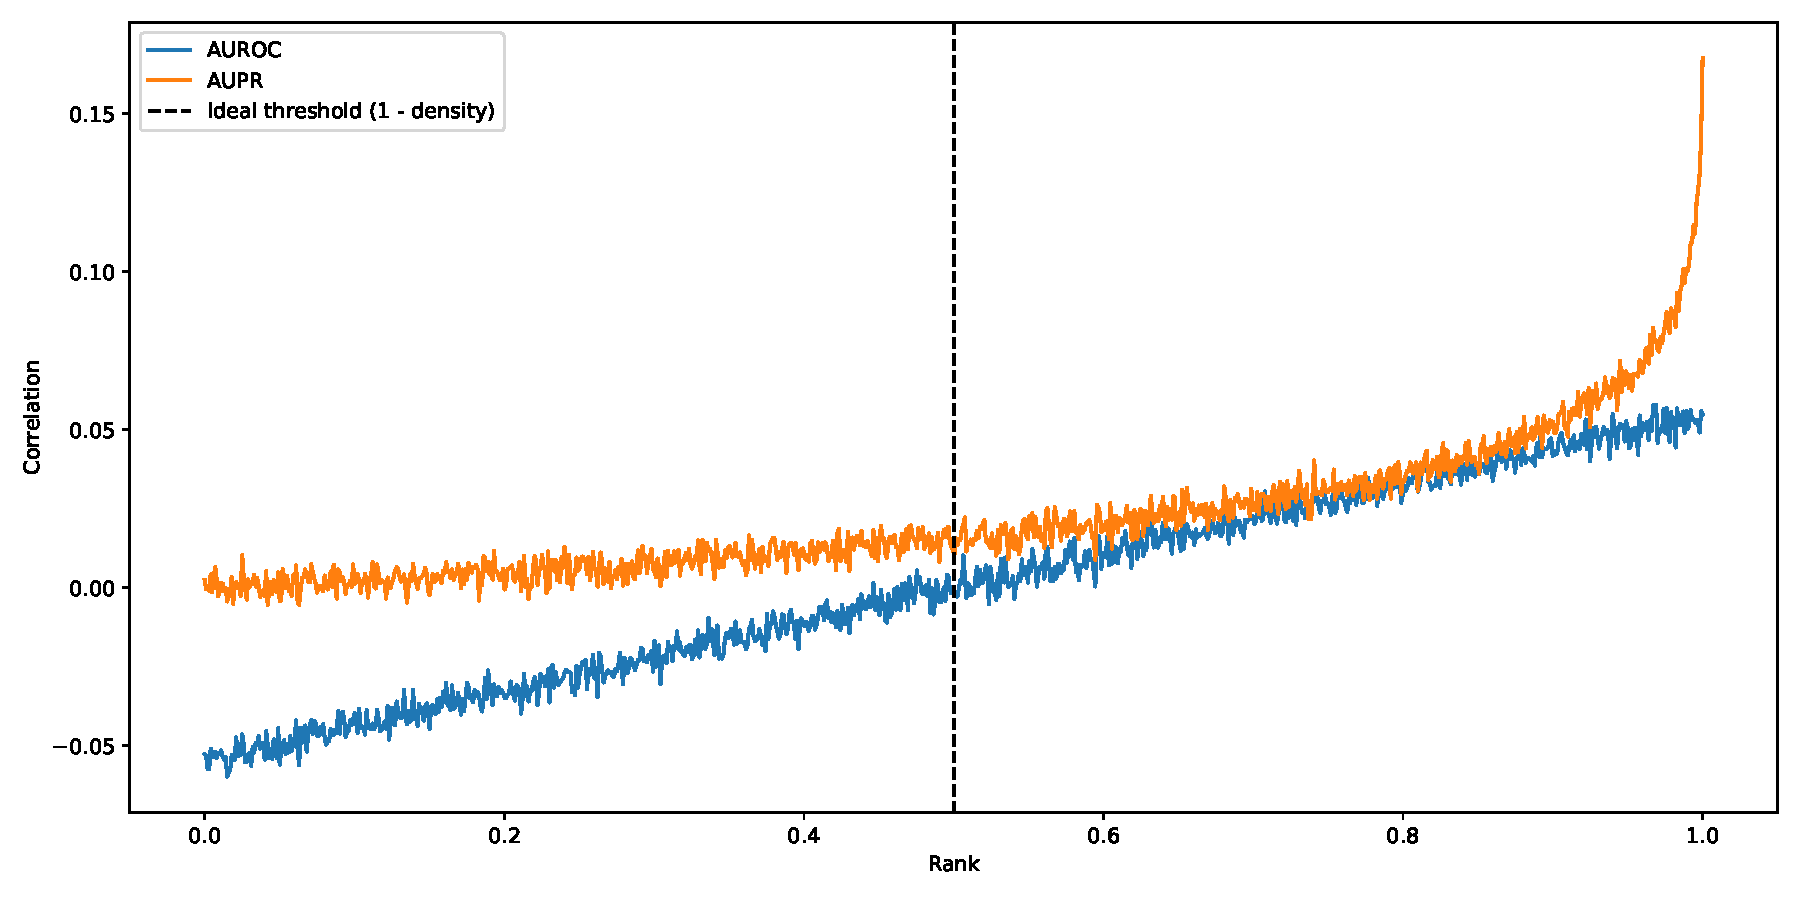
\includegraphics[width=\textwidth]{
        experiments/theoretical_scoring/results/rank_correlation.pdf
    }
    \caption{
        Point biserial correlation between the binary labels at each percentile rank and the AUROC and AUPR scores. The correlation was calculated between the ranks and the scores for $N=10^5$ random sets of $R=10^3$ binary labels. The results show that AUPR is very sensitive to a small group of highest ranks, while AUROC has a more distributed weigthing profile. For AUROC, both higher and lower ranks have a higher impact than ranks around $0.5$, contributing in opposite directions to the final metric. The results confirm the theoretical analyses from \autoref{sec:metrics from ranks}.
        \newline Source: By the author.
    }
    \label{fig:correlation ranks}
\end{figure}

The plot shows that AUPR is highly sensitive to a small set of highest ranks, while ranks closer to $0$ have little influence on the metric. On the other hand, the correlations with the AUROC score are more distributed across ranks. Also, for AUROC, both higher and lower ranks have a higher impact, but in opposite directions.
This behaviour in agreement with the theoretical analyses from \autoref{sec:metrics from ranks}.
The correlation with AUROC is also symmetrical around the median ($r=0.5$), linearly increasing from arround $-0.05$ at $r=0$ to around $0.05$ in $r=1$. This demonstrates the class symmetry of the AUROC metric described in \autoref{sec:metrics from ranks}, meaning that negative and positive labels could be swapped without affecting the final results.
% TODO show that

Overall, these results demonstrate that using AUPR is more suited when one is interested in selecting a restricted number of top-ranked instances from a pool of predictions, such as in recommendation systems or drug discovery tasks.
Conversely, AUROC should be favored when the goal is to rank a large batch of interactions. Examples would be modeling genetic interactions in a genome-wide fashion or building interaction databases.

If one intends to select a small number of negative instances instead, a possible strategy would be to swap the binary labels and use AUPR.
However, one should prioritize AUROC over AUPR if the goal is to select both negative and positive predictions with the highest confidences. This conclusion results from AUPR disregarding ranks close to $0$, so models selected with AUPR are not guaranteed to yield the most confident true negatives.

We also argue that AUROC could be preferable for comparing models under the PU assumption, at least in purely theoretical settings. For PU datasets, we naturally expect some negative-labeled instances to be very highly ranked since they could be, in fact, unannotated positives. AUPR would more strictly penalize such predictions, favoring models that consider the labeling mechanism itself rather than only the underlying interaction mechanism. AUPR could thus undermine the model's potential to discover new interactions, possibly failing to gauge the generalization capabilities of algorithms in a PU context. The results from \autoref{sec:comparison literature} seem to corroborate this hypothesis, with AUROC ranking estimators more consistently than AUPR across different levels of label noise.


\subsection{Are BGSO models faster than GMO models?}
%\subsection{Empirical time complexity analysis}
\label{sec:empirical_complexity}

\begin{mdframed}[frametitle={Key findings}]
    \begin{itemize}
        \item The GMO complexity is measured to be $O(n^3\log n)$, while the BGSO complexity is measured to be $O(n^3)$.

        \item The empirical results match the theoretical expectations from \autoref{sec:complexity_analysis}.
        
        \item The difference in complexity between GMO and GSO is less pronounced for the Extra-Trees, but the GSO models still present significantly lower complexity than the GMO models.
    \end{itemize}
\end{mdframed}

This experiment empirically measures the training time complexity of the tree models under study. We artificially generate a series of bipartite datasets by filling three $n$ by $n$ matrices with pseudo-random values, representing the two $X$ matrices and the $Y$ matrix on each interaction. Values were taken uniformly from the interval $[0, 1]$ for the feature matrices and from the interval $[0, 100]$ for the target matrix.
%We thus represent interactions between $n$ drugs and $n$ proteins, each being described by $n$ features.

We then train the GMO and the optimized GSO versions of a single bipartite decision tree (BDT) and a single bipartite Extra-Tree (BXT) on each of the generated datasets, measuring their training duration in seconds. The results are shown in \autoref{fig:empirical_complexity}. From the least squares linear regression on the log-log plot, we see that the estimated training time complexities closely follow the theoretical expectations developed under Section \ref{sec:complexity_analysis}, with slopes referring to the GSO models (predicted to be $O(n^3)$) approaching 3 while the GMO models (predicted to be $O(n^3\log(n))$) produce slope between 3 and 4.

Statistical testing further shows that the empirical time complexity of the proposed GSO algorithms are indeed significantly lower than that of their GMO counterparts (see the caption for \autoref{fig:empirical_complexity}).

% The value slighly above 3 for bdt\_gso also do not defy expectations, since the theoretical analises were based on the assumption of balanced trees and a small increase in tree depth is expected in real scenarios.

We also notice slightly lower slopes for the Extra-Trees in comparison with the BDTs. In fact, they seem to be closer to the theoretical expectations for the GSO models. This is expected,
since the randomized split search performs far less operations than the exhaustive search (\autoref{sec:split search}). Notwithstanding, both algorithms have the same order of complexity.
%since the bottleneck calculation for these models in the asymptotic regime is the search for the minimum and maximum values of each feature in each node (lines \ref{}), which can be done much faster than the search for the best split employed by the greedy decision trees (\autoref{alg:find_best_split}), even though both procedures have the same order of asymptotic complexity.
%
We then suggest that much larger datasets would be required to observe the asymptotic behavior of the Extra-Trees.
In spite of that, the empirical complexity of \model{bdt-gso} is still observed to be highly significantly lower than that of \model{bxt-gmo}, validating once more the prediction that \model{bdt-gso} should present faster training times than \model{bxt-gmo} on sufficiently large datasets.

\begin{figure}[tb]
    \centering
    \begin{subfigure}{0.49\textwidth}
        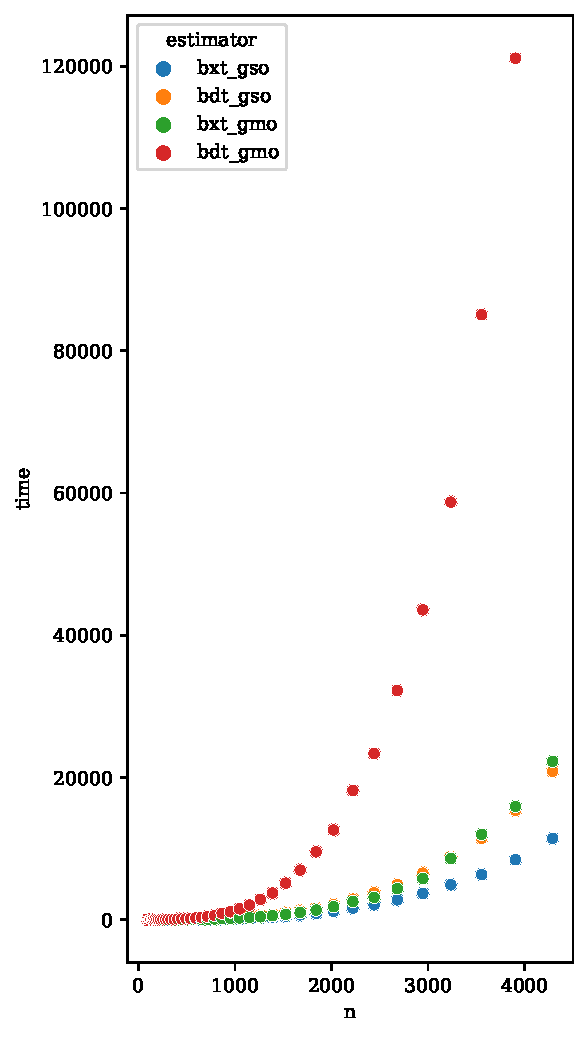
\includegraphics[width=\textwidth]{
            experiments/empirical_complexity/time_vs_n_artificial_data.pdf
        }
    \end{subfigure}
    \begin{subfigure}{0.49\textwidth}
        \includegraphics[width=\textwidth]{
            experiments/empirical_complexity/%
            time_vs_n_artificial_data_loglog.pdf
        }
    \end{subfigure}
    \caption{
        Empirical time complexity estimation of the proposed bipartite global single-output (BGSO) and the global multi-output (GMO)~\cite{pliakos2018global}
        algorithms. Bipartite versions of both extremely randomized trees~\cite{geurts2006extremely} (BXT) and greedy decision trees~\cite{breiman1984classification} (BDT) were built under the GSO and GMO scheme and trained over artificial datasets of varying numbers of samples (as described in \autoref{sec:complexity_analysis}). The training time versus the number of samples is presented on the left. On the right, we present the same plot on a logarithmic scale. The slopes and respective standard deviations are obtained by applying least-squares linear regression.
        Independent two-sample t-tests comparing the slope estimates reveal that the time complexity of \model{bdt-gso} is highly significantly lower than \model{bdt-gmo} ($p < 10^{-64}$) and even \model{bxt-gmo} ($p < 10^{-20}$), and also that \model{bxt-gso} significantly exhibits lower complexity than \model{bxt-gmo} ($p < 10^{-22}$).
        % Those values corroborate the theoretical estimates from \autoref{sec:complexity_analysis}.
        \newline Source: By the author.
    }
    \label{fig:empirical_complexity}
\end{figure}


% \subsection{Comparison between GSO models}  % TODO
% 
% To assess the impact of global single-output optimizations in bipartite decision tree growing, we compare three slightly different training methods for BXT and BRF models.
% 
% \begin{itemize}
%     \item \textbf{ngso}: Naive global single output implementation (Section \ref{});
%     \item \textbf{ngsous}: Naive global single output implementation with undersampling of the non-interacting pairs to yield a balanced training set (Section \ref{});
%     \item \textbf{gso}: Optimized implementation of global single output trees (Section \ref{}).
% \end{itemize}
% 
% While no significant divergence was measured among the GSO models using the entirety of the training data, undersampling revealed to significantly degrade the predictive performance of both forests in terms of AUPR and MCC (Figure \ref{fig:cdd_gso_models}), even though it is arguably the most common procedure when dealing with this kind of data \cite{}.
% 
% On the other hand, AUROC is significantly improved by the undersampling procedure, which is most likely an artifact of the highly imbalanced nature of the present data, as explained as follows. The models grown on the undersampled datasets are naturally the most likely to assign positive labels to new interactions in general, improving TPR at the expense of also increasing FPR. However, since negative labels greatly outnumbers positive labels in the test sets of our current scenario, an increase in FPR impacts a much larger number of predictions than the same increase in TPR. In spite of that, AUROC equally treats TPR and FPR, so that the impact of a high FPR is underestimated. As such, AUROC results could be deemed as unrepresentative of model performance in this setup.
% 
% 
% % TODO: talk about pairwise CV
% 
% When comparing training times, the common choice for undersampling in previous works is justified, as an expressive reduction of training time is observed for both forests (Table \ref{}) relative to naive GSO training. Nevertheless, it is remarkable that the optimized implementation of GSO forests achieves similar training times in comparison to undersampled GSO without the AUPR and MCC burden of undersampling, keeping the higher scores resulting from employing the entirety of the dataset. For larger and less imbalanced datasets, the optimized implementation of GSO forests is expected to be even more advantageous, in agreement with the theoretical time complexity analysis (Section \ref{}).
% 
% %\begin{table}[h]
% %    \input{
% %        figures/experiments/gso_optimization/%
% %        latex_tables/fit.tex
% %    }
% %\end{table}
% 
% In conclusion, the proposed approach confidently enables the use of the entire training data in a much shorter time frame than naive implementations without the need for data undersampling, which is statistically expected to yield better prediction scores for forest predictors.


\subsection{Which prototype should a GMO forest use?}
%\subsection{Comparison between GMO prediction weights}

\label{sec:prototype_comparison}
%TODO: why we did not use BGSO here?

\begin{mdframed}[frametitle={Key findings}]
    \begin{itemize}
        \item The \texttt{square} strategy is the best for both BXT and BRF models, except for the LT+TL AUPR score, for which the fully-grown trees are the best.
        \item The weighted-neighbors strategies seem to improve generalization.
    \end{itemize}
\end{mdframed}

In this work we propose a different prototyping strategy to determine the output value of each leaf in a GMO decision tree, taking the similarity matrices of our use cases into consideration (\autoref{sec:prototype}).
%
In this experiment we compare such strategies, building BXT and BRF models for every option.

The minimum rows per leaf and minimum columns per leaf were both set to 5, ensuring that at least 5 samples of each domain are considered when calculating the prototype values.
%in a weighted-neighbors fashion during evaluation (Section \ref{}).
%
To observe the effect of this early-stopping criterion by itself, we also include forests of fully-grown trees in the comparison. The compared models are described below.

\begin{itemize}
    \item \textbf{\texttt{GMOsa}:} proposed by \citeonline{pliakos2018global}, the output of each leaf is the average of the labels of the learned samples that reach that leaf (\autoref{eq:prototype1}). Their proposal had not been extended yet to ensembles of bipartite trees or to BXT.
    \item \textbf{\texttt{uniform}:} also proposed by \citeonline{pliakos2018global}, but in the context of a single tree. It works as \texttt{GMOsa} for TT, but for TL and LT the average is taken only among the labels of the known instance (\autoref{eq:prototype2}).
    \item \textbf{\texttt{precomputed}:}
    %introduced by us (as also \texttt{square} and \texttt{softmax}),
    the labels in each leaf are weighted by the similarities between the learned samples and the test instances (\autoref{eq:prototype3}).
    \item \textbf{\texttt{square}:} similar to \texttt{precomputed}, but the squared similarities being predicted (\autoref{eq:prototype3}).
    \item \textbf{\texttt{softmax}:} the labels in each leaf are weighted by the exponential of the similarities between the learned samples and the pair being predicted (\autoref{eq:prototype3}).
    \item \textbf{\texttt{full}:} the trees are grown until a single interaction remains in each leaf. %, so that the prediction for each pair is the label of the single learned sample in the leaf.
\end{itemize}

%As shown by \autoref{fig:pred_weights_brf} and Table \ref{}, BXT models show an overall superior performance in comparison to BRF models, with each BXT model scoring significantly higher than its BRF counterpart with the same prediction weights. Furthermore, the weighted GMO predictions seem to prevail relative to the leaf-wise prototype GMOSA (Section \ref{}). Specifically, bxt\_square significantly outperforms all other bipartite forests except for bxt\_precomputed, both in terms of AUROC and average precision (AUPR) in the TT sets (Figure \ref{}).

The results for BRF (\autoref{fig:pred_weights_brf}) and BXT (\autoref{fig:pred_weights_bxt}) were similar. In all cases except LT+TL AUPR, using the square of the similarities to weight the labels in each leaf resulted in in the best scores. For the LT+TL AUPR score, growing the decision tree to its maximal size was the best strategy, followed by \texttt{uniform}, the original proposal by \citeonline{pliakos2018global} of averaging only the 
outputs of the learned samples (known from the training set) in each leaf. With the exception of the LT+TL AUROC metric for BXT, the mentioned winning models were statistically distinguished from all the remaining estimators. For LT+TL AUROC, the superiority of \texttt{square} could not be attested when compared to the \texttt{uniform} strategy.

The fully-grown versions of both forest algorithms are shown to be especially advantageous when considering the LT+TL AUPR. This suggests that building trees to their maximum depth is the best strategy for learning tasks in which
%
\begin{enumerate}
    \item one of the domains is fixed, with the final goal being to model how new instances will bind to this known set of entities;
    \item the goal is to select a small number of top-ranked interactions (see \autoref{sec:comparing auroc aupr}).
\end{enumerate}
%
%Examples that satisfy the first condition are drug repositioning~\cite{} or dyadic prediction~\cite{}. % TODO check
%
On the other hand, weighted averages seem to improve the forest's generalization ability, as they seem to perform best under the AUROC metric and TT contexts.

We propose that this distinction results from the ability of a fully-grown tree to independently consider the labels of each learned instance when calculating the prototype.
However, the methods using weighted averages ivariably mix the labels of a pool of neighbors in each leaf.
This hypothesis is supported by the fact that the second-best model regarding LT+TL AUPR is the \texttt{uniform} strategy, which also uses the labels of individual learned samples to generate the predictions.
%
The hypothesis alone, however, do not explain the superiority of the deeper trees over the \texttt{uniform} weights. In this case, the larger tree depth is likely beneficial through i) an increase in the predictive power of each individual tree, and/or ii) an increase in tree diversity, both of which would improve the ensemble's performance as discussed in \autoref{sec:decision forests}. We let to future work the more specific investigation of these effects.

%The fact the opposite result is found in the TT scenario
On the other hand, \texttt{full} and \texttt{uniform} show notable inferior performance in the TT evaluation settings, suggesting that these strategies have inferior ability to consider completely new interacting pairs.
%the weighting strategy used by the other prototype functions could be an important technique to improve generalization.

%The maximum depth, however, may impact the model's generalization ability, since the same superiority is not shown for the TT AUPR score, where both entities of the pair being predicted are unknown to the model. Our squared-similarity weights seemingly display the best generalization in this regard.

% TODO: why fully grown is not that good for AUROC
%The full models are also seemingly affected

% FIXME: gmosa vs gmo uniform on TT: indicates there are duplicated samples in the dataset, so training samples are leaking to test set.
We select the squared weighting strategy and the fully grown trees to be further investigated in the downstream analyses. %, keeping 5 by 5 as the minimum leaf partition size besides.


\begin{figure}[tb]
    \centering
    \begin{subfigure}{0.49\textwidth}
        \includegraphics{%
            experiments/prediction_weights/statistical_comparisons/%
            brf/all_datasets/boxplots/LT+TL_roc_auc.pdf
        }
    \end{subfigure}
    \begin{subfigure}{0.49\textwidth}
        \includegraphics{%
            experiments/prediction_weights/statistical_comparisons/%
            brf/all_datasets/boxplots/LT+TL_average_precision.pdf
        }
    \end{subfigure}

    \begin{subfigure}{0.49\textwidth}
        \includegraphics{%
            experiments/prediction_weights/statistical_comparisons/%
            brf/all_datasets/boxplots/TT_roc_auc.pdf
        }
    \end{subfigure}
    \begin{subfigure}{0.49\textwidth}
        \includegraphics{%
            experiments/prediction_weights/statistical_comparisons/%
            brf/all_datasets/boxplots/TT_average_precision.pdf
        }
    \end{subfigure}
    \caption{
        Comparison of bipartite random forests for different prototype strategies.
        An omnibus p-value is obtained through a Friedman test and indicated below the title of each subfigure.
        We then perform pairwise Wilcoxon rank-sum tests as a post-hoc analysis.
        Estimators that could \emph{not} be significantly distinguished from each other ($p > 0.05$) are connected by crossbars above their respective boxes. 
        The pairwise test results are corrected by the Benjamini-Hochberg procedure~\cite{benjamini1995controlling,haynes2013benjamini} in each subfigure. All pairwise comparisons are considered for the correction, even if not visible in the plot.
        See \autoref{sec:exp settings} for further description of the evaluation procedure. \newline Source: By the author.
    }
    \label{fig:pred_weights_brf}
\end{figure}


\begin{figure*}[tbh]
    \centering
    \begin{subfigure}{0.49\textwidth}
        \includegraphics[width=\textwidth]{
            experiments/prediction_weights/statistical_comparisons/%
            bxt/all_datasets/boxplots/LT+TL_roc_auc.pdf
        }
    \end{subfigure}
    \begin{subfigure}{0.49\textwidth}
        \includegraphics[width=\textwidth]{
            experiments/prediction_weights/statistical_comparisons/%
            bxt/all_datasets/boxplots/LT+TL_average_precision.pdf
        }
    \end{subfigure}

    \begin{subfigure}{0.49\textwidth}
        \includegraphics[width=\textwidth]{
            experiments/prediction_weights/statistical_comparisons/%
            bxt/all_datasets/boxplots/TT_roc_auc.pdf
        }
    \end{subfigure}
    \begin{subfigure}{0.49\textwidth}
        \includegraphics[width=\textwidth]{
            experiments/prediction_weights/statistical_comparisons/%
            bxt/all_datasets/boxplots/TT_average_precision.pdf
        }
    \end{subfigure}
    \caption{
        Comparison of bipartite Extra-Trees for different prototype strategies.
        An omnibus p-value is obtained through a Friedman test and indicated below the title of each subfigure.
        We then perform pairwise Wilcoxon rank-sum tests as a post-hoc analysis.
        Estimators that could \emph{not} be significantly distinguished from each other ($p > 0.05$) are connected by crossbars above their respective boxes. 
        The pairwise test results are corrected by the Benjamini-Hochberg procedure~\cite{benjamini1995controlling,haynes2013benjamini} in each subfigure. All pairwise comparisons are considered for the correction, even if not visible in the plot.
        See \autoref{sec:exp settings} for further description of the evaluation procedure. \newline Source: By the author.
    }
    \label{fig:pred_weights_bxt}
\end{figure*}



\subsection{Which adaptation strategy is the best for decision forests?}
\label{sec:adaptation_comparison}

\begin{mdframed}[frametitle={Key findings}]
    \begin{itemize}
        \item SLMO is the best strategy for BRF models on LT+TL sets.
        \item GMO is the best strategy for completely new dyads.
        \item Undersampling of negative annotations is beneficial for GSO BXT in terms of AUROC, but should be avoided if the goal is to select the highest ranked interactions.
    \end{itemize}
\end{mdframed}

We now compare each of the described approaches for adapting decision forests to bipartite data, including data-centric adaptations (\autoref{sec:standard adaptations}) and the natively bipartite forests (\autoref{sec:bipartite_trees} and \autoref{sec:bgso_trees}). We briefly describe below the suffixes in the model names of this section, indicating the employed bipartite adaptations.

% TODO: contribution: ensembles of gmo (not gmosa) were nevel built!

\begin{itemize}
    \item \textbf{\texttt{lmo}:} implements the standard local multi-output approach (SLMO; \autoref{sec:slmo}) by training four separate multioutput models, two for each domain. First explored by \citeonline{schrynemackers2015classifying}.
    \item \textbf{\texttt{lso}:} also implements the SLMO approach (\autoref{sec:slmo}), but each multioutput model is instead a composition of several local single-output (LSO) models, i.e. one model is trained for each row or column of the interaction matrix. This setting is similar to the early proposal by \citeonline{bleakley2009supervised}, but employing decision forests as the base algorithm.
    \item \textbf{\texttt{gmosa}:} a global multi-output forest with single-label averaging (GMOSA; \autoref{sec:prototype}), as explored by \citeonline{pliakos2019network} under the name eBICT.
    \item \textbf{\texttt{gmo}:} a global multi-output (GMO; \autoref{sec:bipartite_trees}) forest with minimum leaf dimensions of 5 by 5, implementing our proposed squared-similarities weighting for the prototype function (\autoref{sec:prototype}). Apart from the new prototype, this model is based on the original GMO trees proposed by \citeonline{pliakos2018global}. Despite their original results suggesting advantage over GMOSA, to the best of our knowledge, this is the first time the GMO trees are employed in building decision forests.  % TODO explain GMOSA
    \item \textbf{\texttt{gso}:} a bipartite global single-output (BGSO; \autoref{sec:bgso_trees}) forest, as initially explored by \citeonline{schrynemackers2015classifying} but now implementing our proposed algorithm with improved computational complexity.
    \item \textbf{\texttt{sgso\_us}:} implements the standard global single-output (SGSO; \autoref{sec:sgso}) adaptation, additionally employing undersampling of the non-interacting pairs to yield a balanced training set (\autoref{sec:sgso}).  % TODO explain that is frequently used
\end{itemize}

All the global models were built with 100 trees. For SLMO, each of the four forests used 50 trees, while for LSO 50 trees were used for each row or column of the interaction matrix.

In the LT+TL AUPR evaluation setting, the pattern observed in \autoref{sec:prototype_comparison} again emerges: the label averaging strategy employed by GMO performs considerably worse in comparison to forests that separately consider each known instance. In particular, the SLMO and SLSO adaptations yield the clear best BRF models in terms of LT+TL AUPR, and these adaptations interpret each instance as a separate output to be predicted. Among the local adaptations, SLMO significantly ouperforms SLSO. SLSO treats each training instance as a completely independent task, building a separate forest for each row and column of the interaction matrix. As such, the previous result shows that this complete independence is not desirable for the learning problems under study, and exploring label correlations between instances of the same domain is beneficial (as demonstrated by SLMO). This result could partially be a consequence of the very sparse nature of our problems: if the interaction information of each instance is limited, it becomes advantageus to aggregate information from other instances with correlated interactomes. We then speculate that the advantage of SLMO over SLSO could become less prominent once the number of known interactions per instance increases and more data are available for training.

Still considering LT+TL AUPR but focusing on BXT models instead, we notice that SLMO loses the advantage to the fully-grown bipartite trees GMO and GSO. A possible explanation comes from the fact that local approaches yield shallower trees, and much more extra-trees could be required to achieve comparable performance. In more detail, first notice that the individual performance of each tree in a BXT forest is lower than that of a tree in a BRF. Thus, a BXT ensemble requires a larger number of trees to reach satisfactory performance. Additionally, if the trees are shallow, they tend to be less representative of the training data (each tree node brings a little more information on the dataset).
Even more trees then should be required to compensate the randomness of each individual. Finally, building a forest locally as in SLMO or SLSO results that each tree is trained on a much smaller number of samples in comparison to considering each dyad as a separate instance. Therefore, local approaches generate smaller and less representative trees. We then suggest that the advantage of SLMO could also manifest for BXT estimators if the number of trees in the ensemble were to be increased.

For both BXT and BRF in all the TT settings, the GMO model significantly outperforms the other estimators. GMO is also the best model in the LT+TL AUROC setting when comparing BXTs and the second best for BRFs. This reinforces the findings of \autoref{sec:prototype_comparison} suggesting that larger leaves and label weighting seems to improve generalization to unseen instances.
%
We also highlight SLMO as a prominent strategy for BRFs under TT AUROC and TT AUPR, being the second best model in both cases.

The SGSO US strategy performed consistently worse than the others under the AUPR metric. Conversely, it was significantly the second best BXT model in both LT+TL and TT AUROC settings, while surpassing BRF GMOSA also under both AUROC test sets.
This shows that unsersampling is a viable technique when when considering the overall ranking of interactions. However, it is detrimental when the goal is to select the most likely interactions. That is, SGSO US allows a larger number of false positives in the highest ranked positions.

This behaviour is expected. Notice that SGSO US models are trained in a balanced dataset, while the other models are trained in the original dataset where negative annotations are much more frequent. With more training examples, the other models tend to be considerably better in correctly classifying negative annotations. This suggests that AUPR tends to favor models of high specificity, that are strictly avoid predicting false positives.
%The explanation would be that the undersampling procedure naturally causes the model to equally prioritize the positive and negative labels, which matches the AUROC's behaviour of equally treating TPR and FPR.
%More specifically, these models tend to produce a larger number of false positives since they are unaware of the large label imabalance of our test sets. While this substantially affects AUPR, the AUROC metric is agnostic to the label imbalance (\autoref{sec:prediction_metrics}), being much more forgiving with the number of false positives given the large total number of negative labels in the test sets.

% TODO sgso us is popular but not good

%We select LMO, GMO, GSO, and GMOSA to be further analysed in the next section.

% TODO: relationship with previous work

% The GMO approach is also highlighted by the results of BXT ensembles, being undisputed for the LT+TL AUROC and TT scores. Interestingly, for the LT+TL AUPR score, its mean percentile ranking was the second to last, being only better than SGSOUS. These results corroborate the idea discussed in \autoref{sec:prototype_comparison} that reaching the maximum tree depth is the best strategy for LT+TL, 

% TODO training times

% To avoid differences in random sampling when using the naive GSO adapter versus the natively bipartite GSO tree, no bootstraping was applied to any forest, providing all trees with the whole training samples space. To still ensure randomization in random forest estimators, the maximum features parameter was set to $0.5$, meaning that each tree in a random forest was trained on a random subset of half the features from each sample domain. Due to implementation details, this means the naive GSO forests will sample features slightly differently: they will pick half the features from the whole feature space combined, while the natively bipartite GSO forests will ensure half the features from each sample domain is selected. This is not expected to have a significant impact on the results, given that the total number of features is especially high in the present scenario, where similarity matrices are being employed. 

%All forests were composed of 100 tree estimators and were fully grown, with the exception of the GMO models, whose leaf sizes were limited to a minimum of 5 by 5 samples (at least 5 samples from each domain) in order to take advantage of neighborhood weighting (which was set to the squared similarities, see Section \ref{}).

%In all of the evaluated scenarios, a BXT model was ranked the best. In both TT-MCC and TL-AUPR, the BRF models and bxt\_gmo were significantly surpassed by the remaining BXT forests. In TL-MCC, bxt\_lso significantly outperformed all the other models. Given that this test-set provides the greatest intersection with the training set, due to the overall higher number of column samples in the datasets we used, we suggest that the LSO model could be better at taking advantage of already seen information from a sample domain, since a forest is grown separately for each row and column. From another perspective, this effect could be regarded as a form of overfitting. This hypothesis is further supported by the fact that both GMO models, which were the only forests subject to a minimum leaf size constraint and thus less prone, in theory, to overfitting, were the most frequently outperformed models in the TL-MCC and TL-AUPR.

%Contrastingly, both GMO models were consistently the best performing models in all AUROC settings, which is commonly assumed to be a less indicative metric in highly imbalanced classification contexts such as the present one \cite{}. This could be explained by a bias towards the majority class, possibly caused by the averaging of the larger leaves employed in this methods. %FIXME: actually, a bias towards minority class

\begin{figure}[tb]
    \centering
    \begin{subfigure}{0.49\textwidth}
        \includegraphics[width=\textwidth]{
            experiments/bipartite_adaptations/statistical_comparisons/%
            brf/all_datasets/boxplots/LT+TL_roc_auc.pdf
        }
    \end{subfigure}
    \begin{subfigure}{0.49\textwidth}
        \includegraphics[width=\textwidth]{
            experiments/bipartite_adaptations/statistical_comparisons/%
            brf/all_datasets/boxplots/LT+TL_average_precision.pdf
        }
    \end{subfigure}

    \begin{subfigure}{0.49\textwidth}
        \includegraphics[width=\textwidth]{
            experiments/bipartite_adaptations/statistical_comparisons/%
            brf/all_datasets/boxplots/TT_roc_auc.pdf
        }
    \end{subfigure}
    \begin{subfigure}{0.49\textwidth}
        \includegraphics[width=\textwidth]{
            experiments/bipartite_adaptations/statistical_comparisons/%
            brf/all_datasets/boxplots/TT_average_precision.pdf
        }
    \end{subfigure}
    \caption{
        Comparison of random forests under different adaptation strategies to bipartite interaction data.
        An omnibus p-value is obtained through a Friedman test and indicated below the title of each subfigure.
        We then perform pairwise Wilcoxon rank-sum tests as a post-hoc analysis.
        Estimators that could \emph{not} be significantly distinguished from each other ($p > 0.05$) are connected by crossbars above their respective boxes. 
        The pairwise test results are corrected by the Benjamini-Hochberg procedure~\cite{benjamini1995controlling,haynes2013benjamini} in each subfigure. All pairwise comparisons are considered for the correction, even if not visible in the plot.
        See \autoref{sec:exp settings} for further description of the evaluation procedure. \newline Source: By the author.
    }
    \label{fig:adaptations_brf}
\end{figure}


\begin{figure}[tb]
    \centering
    \begin{subfigure}{0.49\textwidth}
        \includegraphics[width=\textwidth]{
            experiments/bipartite_adaptations/statistical_comparisons/%
            bxt/all_datasets/boxplots/LT+TL_roc_auc.pdf
        }
    \end{subfigure}
    \begin{subfigure}{0.49\textwidth}
        \includegraphics[width=\textwidth]{
            experiments/bipartite_adaptations/statistical_comparisons/%
            bxt/all_datasets/boxplots/LT+TL_average_precision.pdf
        }
    \end{subfigure}

    \begin{subfigure}{0.49\textwidth}
        \includegraphics[width=\textwidth]{
            experiments/bipartite_adaptations/statistical_comparisons/%
            bxt/all_datasets/boxplots/TT_roc_auc.pdf
        }
    \end{subfigure}
    \begin{subfigure}{0.49\textwidth}
        \includegraphics[width=\textwidth]{
            experiments/bipartite_adaptations/statistical_comparisons/%
            bxt/all_datasets/boxplots/TT_average_precision.pdf
        }
    \end{subfigure}
    \caption{
        Comparison of Extra-Trees under different adaptation strategies to bipartite interaction data.
        An omnibus p-value is obtained through a Friedman test and indicated below the title of each subfigure.
        We then perform pairwise Wilcoxon rank-sum tests as a post-hoc analysis.
        Estimators that could \emph{not} be significantly distinguished from each other ($p > 0.05$) are connected by crossbars above their respective boxes. 
        The pairwise test results are corrected by the Benjamini-Hochberg procedure~\cite{benjamini1995controlling,haynes2013benjamini} in each subfigure. All pairwise comparisons are considered for the correction, even if not visible in the plot.
        See \autoref{sec:exp settings} for further description of the evaluation procedure. \newline Source: By the author.
    }
    \label{fig:adaptations_bxt}
\end{figure}


\subsection{Can label imputation assist bipartite forests?}
\label{sec:y_reconstruction}

\begin{mdframed}[frametitle={Key findings}]
    \begin{itemize}
        \item Imputing positive annotations with NRLMF improves the performance of bipartite forests in the majority of cases.
        \item For LT+TL AUPR, the best BRF is \model{BRF-LMO} and the best BXT is \model{BXT-GMOSA-NRLMF}.
        % \item For LT+TL AUROC, the best BRF is \model{BRF-LMO-NRLMF}
        \item GMO NRLMF is the overall best model for TT.
    \end{itemize}
\end{mdframed}

In this section, we compare bipartite forests with and without label imputation by matrix factorization. We employ the adaptations SLMO, GMO, BGSO, and GMOSA based on the results of \autoref{sec:adaptation_comparison}.

It was previously suggested that creating a dense representation of the interaction matrix improves the performance of BXT in drug-target interaction tasks~\cite{pliakos2020drugtarget}.
To test this result on our datasets, we compare the bipartite forests scores with and without the interaction matrix reconstruction step. As \cite{pliakos2020drugtarget}, the reconstruction step was performed using neighborhood-regularized logistic matrix factorization (NRLMF)~\cite{liu2016neighborhood}.

%\subsubsection{Hyperparameter selection}
%\subsubsection{Experimental settings}
We performed a randomized search to select hyperparameters for the NRLMF algorithm. 100 different combinations of hyperparameters were evaluated
in terms of their resulting mean squared error in a nested bipartite 5-fold diagnonal cross-validation.
The best combination of parameters according to the inner CV loop was then used to reconstruct the interaction matrix of each outer CV fold. Only then the resulting matrices were used as the training data for the bipartite forests. Note that a single forest was built per outer CV fold, so that the NRLMF hyperparameter search was performed independently from the downstream forest performance.
% The hyperparameters \texttt{lambda\_rows}, \texttt{lambda\_cols}, \texttt{alpha\_cols}, \texttt{alpha\_cols}, and \texttt{learning\_rate} were all independently sampled from a log-uniform distribution bounded by $\frac{1}{4}$ and $2$.
The hyperparameters $\lambda_1$, $\lambda_2$, $\beta_1$, $\beta_2$, and $\eta$ were all independently sampled from a log-uniform distribution bounded by $\frac{1}{4}$ and $2$ (\autoref{alg:nrlmf_train}).
The number of latent vector components was set to be equal for both axes, and chosen between 50 and 100. The number of neighbors was randomly selected as 3, 5 or 10 in each iteration, and the maximum number of optimization steps was always set to 100. The parameter $\alpha$ (\autoref{alg:nrlmf_train}), as in the original paper~\cite{liu2016neighborhood}, was set to $5$. This parameter specifies the emphasis on positive annotations, so each positive annotation contributes $5$ times more to the loss function in our settings, as if 5 copies of each positive interaction were present in the training set.
%
See \autoref{sec:adaptation_comparison} for descriptions on the bipartite forests being compared.

The results for BRF and BXT are shown by figures \ref{fig:brf_y_reconstruction} and \ref{fig:bxt_y_reconstruction}, respectively. The \texttt{nrlmf} suffix to a model indicates that it was built on the output of NRLMF.

The interaction matrix reconstruction step is shown to be especially beneficial in terms of AUROC scores, improving this score for almost all forest algorithms investigated. The only exceptions were \model{bxt-gmo} and \model{brf-gmo} in LT+TL ROC AUC, where the improvement is still observed but not statistically significant.
%
%As discussed in \autoref{sec:comparing auroc aupr}, ROC AUC is characterized by more leniency towards highly-ranked false positives, which explains the advantage posed by NRLMF in this setting: NRLMF explicitly defines a parameter to prioritize outputting positive interactions (\autoref{sec}). % TODO
%
%In accordance with previous investigations~\cite{liu2016neighborhood,liu2017lpinrlmf,liu2020predicting,pliakos2020drugtarget},
%this parameter was set to 5, meaning that the loss function employed in the gradient descent procedure of NRLMF is weighted 5 times more for positive interactions than for negative interactions, as if 5 copies of each positive interaction were present in the training set.

Even without the help from NRLMF, the \model{bxt-gmo} and \model{brf-gmo} models employing our squared similarities output weighting (sections \autoref{sec:prototype} and \autoref{sec:prototype_comparison}) are placed second in their corresponding TT ROC AUC results, both significantly outperforming all NRLMF-combined models except for their own versions, \model{bxt-gmo-nrlmf} and \model{brf-gmo-nrlmf}. % (as aforementioned).
\model{brf-gmo} was also the top performing BRF model in terms of TT AUPR, significantly surpassing all but \model{brf-gmo-nrlmf} and \model{brf-lmo-nrlmf}.
Similarly, \model{bxt-gmo} was the top performing BXT model under the same metric, significantly surpassing all estimators but \model{bxt-gmo-nrlmf}, \model{bxt-lmo-nrlmf} and \model{BXT-GMOSA-NRLMF}.

Regarding TT AUPR, NRLMF still provides a significant improvement for all models except \model{brf-gmo}, \model{bxt-gmo} and \model{bxt-lmo}. While both BRF GMO and BXT GMO resulted in the highest average ranks for TT AUPR, the top position could not be statistically resolved between the BRFs using GMO, GMO NRLMF, and LMO NRLMF, nor between the BXTs using GMO, GMO NRLMF, LMO NRLMF, and GMOSA NRLMF.

In the LT+TL AUPR setting for BXT ensembles, NRLMF is shown to significantly degrade the performance of \model{bxt-gmo}. Therefore, the combination of the squared neighbors prototype and NRLMF likely results in more high-rank false positives under LT+TL, especially since such degradation is not observed under LT+TL AUROC.  % TODO name prototype
%
%We attribute this effect to the aforementioned increase in false positives caused by NRLMF, especially since such degradation is not observed under LT+TL AUROC. Notwithstanding, we note that this degradation of LT+TL AUPR is exclusive to the GMO adaptation, as all other BXT models are significantly improved by NRLMF in this setting. Moreover, we highlight the differences between the LT+TL AUROC and LT+TL AUPR results considering BXT GMO and \model{BXT-GMO-NRLMF}: while these models are the best ranked in the former setting, they are the clear worst in the latter. We thus argue that both the GMO strategy and the NRLMF reconstruction step, each in and of itself, have the effect of increasing the tendency towards false positives in the predictions. Their summed effects could thus impair predictive performance especially under LT+TL AUPR evaluation, whereas in other settings they could  missing positives or AUROC evaluation in general, the combina...  % TODO finish this discussion

%This suggests that the combination of GMO's label averaging method 

% TODO: (last section) gmo more fp

% Interestingly, the scores for \model{bxt-gmo}, \model{brf-gmo}, and \model{brf-lmo} are instead significantly reduced by combination with the matrix factorization technique in LT+TL AUPR, contrary to the overall tendency.
%

For BRF models under LT+TL AUPR, the advantage of employing NRLMF is not clear. GSO was the only adaptation to significantly benefit from NRLMF in this setting, while GMO and LMO were significantly impaired by it. In fact, the \model{BRF-LMO} model without label matrix reconstruction significantly outperformed all the other random forests for this evaluation setting.

% Not clear from the data:
%Additionally, the GSO and GMOSA models are seemingly favored by the LT+TL setting in comparison to TT, reinforcing the results of \autoref{sec:adaptation_comparison} suggesting that deeper trees are advantageous for LT+TL, while the larger leaves of GMO models seem to improve generalization for completely unknown pairs (TT AUPR). Notably, the \model{bxt-gmosa-nrlmf} model, proposed by \citeonline{pliakos2020drugtarget} under the name of BICTR, was the top scoring model among BXT for all but the TT ROC AUC test settings.

% TODO add hue, compare within pairs with vs without nrlmf
% TODO
% fullly grown doesnt mean n_leaf == 1
% we expect more trees to make nrlmf irrelevant
% nrlmf probably makes more false positives
% less relevant for gmo and degrades performance in lttl AUPR only for rf
% complexity of other adaptations
% why nrlmf is detrimental to BRF lt+tl AUPR?
% why nrlmf is detrimental to GMO?
% why nrlmf is not detrimental to bxt lmo?

%So why does NRLMF seem detrimental to \model{brf-gmo}, \model{bxt-gmo} and \text{brf-lmo} in terms of LT+TL AUPR? For any tree, if one of the interacting entities is known from the training data (let's call it $\x_\text{known}$), the leaf at which the interaction from the TL or LT sets arrives is guaranteed to hold a partition of $Y_\text{train}$ with a column corresponding to $\x_\text{known}$. The GMO and LMO models are the only ones to emphasize the effect of this column: LMO will output the average of only the labels in this column (see \autoref{sec:slmo}), while GMO will weight it considerably higher than the other columns when computing the leaf's prototype (\autoref{sec:prototype}). The usage of NRLMF however, causes the negative labels in such column of $Y_\text{leaf}$ to be influenced by neighbors from the training set. While this should improve generalization, we speculate that the LT+TL setting could benefit from this "partial overfitting" that occurs when NRLMF is not employed. We thus hypothesize this effect is less pronounced in BXT due to the naturally lower tendency to overfit of Extra-Trees, resulting from the randomized selection of thresholds (\autoref{sec:bipartite_forests}). We also suppose that this effect in LT+TL ROC AUC is overruled by the sensitivity improvement brought by NRLMF, as discussed above, hence it not being apparent from the results.

%Another hypothesis can be formulated based on the fact that the dense reconstructed matrix will cause trees to grow to a much deeper extent.
%%as homogeneity of leaves is harder to obtain.
%As such, this could favor overfitting of BRF models to the output of NRLMF, carrying the generalization error of the NRLMF reconstruction to the results. At the same time, NRLMF being a better model than BRF on TT sets would generate, as observed, the inverse effect, with NRLMF improving performance in this case. % TODO discuss this in model comparison section
%% this would cause BRF to be equal or worse than NRLMF alone
%Again, BXT's randomized split search procedure likely makes it more resilient to this influence, building uncorrelated individual estimators even if the trees are large and thus more generally benefitting from NRLMF.

% TODO
%On BXT, Based on these hypothesis, we predict that the impact of NRLMF will be less prominent on a greater number of trees

% Additionally, imputting the negative labels allows the trees to grow deeper

%\model{brf-gmo} and \model{lmo} are the models most likely to overfit the training data, given that 

%We speculate that the addition of the NRLMF training step does introduce more information into the training set, of which downstream trees can take advantage, at the expense of elevating type I errors and reducing estimator variance. The first effect, increasing FPR, could explain the positive effect of NRLMF on ROC AUC, as aforementioned...

% The second effect would be to decrease the correlation of each tree with the original interaction matrix.

% nrlmf and gmo
% TODO: future testing with less positive importance and larger trees
% some of the estimators are definitely not calibrated (explain)

In summary, interaction matrix reconstruction by NRLMF seems to consistently improve BRF and BXT results in terms of AUROC and also the results of BXT regarding LT+TL AUPR. On TT AUPR, while less evidence is found, the results still seem to point in the same direction of a beneficial NRLMF transformation step. On the other hand, the comparisons of BRF under LT+TL AUPR evaluation indicate the opposite conclusion, disfavoring usage of NRLMF especially for \model{brf-lmo} and \model{brf-gmo}. We thus discourage the application of NRLMF with BRF in scenarios where i) one of the entities of the dyad is always known to the model, such as in drug repositioning; and ii) the main interest is to select a small set of most-likely interactions.

% TODO: remake the following explanation after displaying the rank boxplots

% A first explanation could be that the NRLMF hyperparameter search was not exhaustive enough, and that a better combination of hyperparameters could have been found. However, we later show in section \ref{} that the NRLMF model alone displays competitive performance, disfavoring such hypothesis of underfitting.
% 
% We also notice that \cite{Liu_2017} performs bipartite cross-validation in unusual fashion, by replacing with zeros the positive labels of pairs assigned to the test set but still using them to train the model. Albeit test labels are masked, each model thus still receives all available samples during training, and we hypothesize that unsupervised information from the test set could possibly still be exploited during training. For instance, estimating the sample density of the feature space could provide an importance score, a weight factor, for each sample, in order to favor correct predictions of denser clusters and undermine outliers. Wether and how this or similar mechanisms are explored by the NRLMF algorithm is out of the scope of this work, but we discourage the use of such CV strategy and point it as a possible reason for the higher NRLMF scores observed by previous authors \cite{Pliakos_2020;Liu_2017}.

% (False, they also used nested CV) The authors of \cite{Pliakos_2020} also do not clearly specify the could have employed the reconstruction step before splitting the data into the cross-validation folds, in which case the observed performance improvement could be attributed to indirect data leakage, where the labels used to train the downstream forest estimator were generated from neighbor samples that are possibly in the test sets.

\begin{figure}[tb]
    \centering
    \begin{subfigure}{0.49\textwidth}
        \includegraphics[width=\textwidth]{
            experiments/y_reconstruction/statistical_comparisons/%
            brf/all_datasets/boxplots/LT+TL_roc_auc.pdf
        }
    \end{subfigure}
    \begin{subfigure}{0.49\textwidth}
        \includegraphics[width=\textwidth]{
            experiments/y_reconstruction/statistical_comparisons/%
            brf/all_datasets/boxplots/LT+TL_average_precision.pdf
        }
    \end{subfigure}

    \begin{subfigure}{0.49\textwidth}
        \includegraphics[width=\textwidth]{
            experiments/y_reconstruction/statistical_comparisons/%
            brf/all_datasets/boxplots/TT_roc_auc.pdf
        }
    \end{subfigure}
    \begin{subfigure}{0.49\textwidth}
        \includegraphics[width=\textwidth]{
            experiments/y_reconstruction/statistical_comparisons/%
            brf/all_datasets/boxplots/TT_average_precision.pdf
        }
    \end{subfigure}
    \caption{
        Comparison of bipartite random forests with and without label imputation by NRLMF.
        An omnibus p-value is obtained through a Friedman test and indicated below the title of each subfigure.
        We then perform pairwise Wilcoxon rank-sum tests as a post-hoc analysis.
        Estimators that could \emph{not} be significantly distinguished from each other ($p > 0.05$) are connected by crossbars above their respective boxes. 
        The pairwise test results are corrected by the Benjamini-Hochberg procedure~\cite{benjamini1995controlling,haynes2013benjamini} in each subfigure. All pairwise comparisons are considered for the correction, even if not visible in the plot.
        See \autoref{sec:exp settings} for further description of the evaluation procedure. \newline Source: By the author.
    }
    \label{fig:brf_y_reconstruction}
\end{figure}


\begin{figure}[tb]
    \centering
    \begin{subfigure}{0.49\textwidth}
        \includegraphics[width=\textwidth]{
            experiments/y_reconstruction/statistical_comparisons/%
            bxt/all_datasets/boxplots/LT+TL_roc_auc.pdf
        }
    \end{subfigure}
    \begin{subfigure}{0.49\textwidth}
        \includegraphics[width=\textwidth]{
            experiments/y_reconstruction/statistical_comparisons/%
            bxt/all_datasets/boxplots/LT+TL_average_precision.pdf
        }
    \end{subfigure}

    \begin{subfigure}{0.49\textwidth}
        \includegraphics[width=\textwidth]{
            experiments/y_reconstruction/statistical_comparisons/%
            bxt/all_datasets/boxplots/TT_roc_auc.pdf
        }
    \end{subfigure}
    \begin{subfigure}{0.49\textwidth}
        \includegraphics[width=\textwidth]{
            experiments/y_reconstruction/statistical_comparisons/%
            bxt/all_datasets/boxplots/TT_average_precision.pdf
        }
    \end{subfigure}
    \caption{
        Comparison of bipartite Extra-Trees with and without label imputation by neighborhood-regularized logistic matrix factorization.
        An omnibus p-value is obtained through a Friedman test and indicated below the title of each subfigure.
        We then perform pairwise Wilcoxon rank-sum tests as a post-hoc analysis.
        Estimators that could \emph{not} be significantly distinguished from each other ($p > 0.05$) are connected by crossbars above their respective boxes. 
        The pairwise test results are corrected by the Benjamini-Hochberg procedure~\cite{benjamini1995controlling,haynes2013benjamini} in each subfigure. All pairwise comparisons are considered for the correction, even if not visible in the plot.
        See \autoref{sec:exp settings} for further description of the evaluation procedure. \newline Source: By the author.
    }
    \label{fig:bxt_y_reconstruction}
\end{figure}



\subsection{What is the best way of building semi-supervised forests?}
\label{sec:ss_comparison}

\begin{mdframed}[frametitle={Key findings}]
    \begin{itemize}
        \item The MD unsupervised impurity is the best option for LT+TL.
        \item AD is the most promising strategy for TT.
        \item The best strategy for determining the supervision balance seems to be either size or fixed, but further investigation is needed.
    \end{itemize}
\end{mdframed}

In this experiment, we compare the performances of semi-supervised bipartite forests \autoref{sec:ss trees}. All forests in this section are based on the BGSO BXT, as described in \autoref{sec:adaptation_comparison}. We evaluate all combinations of the three strategies for calculating the unsupervised impurity and the four strategies for determining the supervision balance at each node.

\paragraph*{Strategies for determining the unsupervised impurity:}
\begin{itemize}
    \item \textbf{\texttt{mse}:} it refers to forests using the mean squared error as the unsupervised impurity (\autoref{eq:I u mse}).
    \item \textbf{\texttt{md}:} corresponds forests employing the mean distance unsupervised impurity (\autoref{eq:mean distance impurity}).
    \item \textbf{\texttt{ad}:} also uses the mean squared error (\autoref{eq:I u mse}), however, the semi-supervised impurity is only calulated twice on each tree node. The search for the best feature and split point in each instance domain uses the supervised impurity only. Then, the semi-supervised impurity is only used to evaluate the best split in each domain. Finally, the two resulting values for the semi-supervised impurity are used to select between the horizontal and vertical split.
\end{itemize}

\paragraph*{Strategies for determining the supervision balance ($\sigma$):}
\begin{itemize}
    \item \textbf{\texttt{fixed}:} the supervision balance ($\sigma$) is fixed at $0.5$ for mse and md and at $0$ for ad.
    \item \textbf{\texttt{density}:} $\sigma$ is determined by the density of positive annotations in each tree node (\autoref{eq:sigma density}). 
    \item \textbf{\texttt{size}:} $\sigma$ is determined by the total number of interactions current in the tree node (\autoref{eq:sigma size}).
    \item \textbf{\texttt{random}:} $\sigma$ is set to a random value between $0$ and $1$ drawn at each tree node (\autoref{eq:sigma random}).
\end{itemize}

The comparison results are displayed by \autoref{fig:ss_comparison}.
%
Regarding LT+TL AUROC, the 0\% ILR and 50\% ILR do not result in statistically significant differences in performance. For ILR = 70\%, md random and md size significantly outperform the remaining models, while under IRL=90\%, md random, md size, and md density are shown to surpass the others. These results indicate that the MD unsupervised impurity is the most suited to the LT+TL AUROC evaluation setting. Furthermore, we see that the random strategy to select the supervision balance %TODO
is among the best in both ILR = 70\% and ILR = 90\%, suggesting that increasing diversity among the trees could be the main mechanism behind the improvement of the semi-supervised models, rather than necessarily guessing the best $\sigma$ at each tree node. Since md size is also among the best, it is not clear if the advantage of md size over the other models is due to a better choice of $\sigma$ or to a more stochastic nature of the $\sigma$s it selects.
%
%As a future investigation, we suggest using the size-based $\sigma$ selection with a completely random unsupervised impurity, .
%
As a future investigation, we suggest using completely random values for the unsupervised impurity, to assess the possibility of tree-diversity being the main factor behind the observed improvements.

As for TT AUROC, only ILR = 90\% yielded significant comparisons. In this case, the mse unsupervised impurity with size, random, and density $\sigma$ selection were the best strategies, surpassing the remaining. MSE thus seems the better option in terms of AUROC for scenarios with very scarse information and completely unknown instances.

Under LT+TL AUPR, md fixed significantly outperformed the other models for ILR = 50\% and ILR = 70\%. For ILR = 0\%, md fixed is also the first place, but could not be statistically resolved from the second place ad size. AD size was also the second best model for ILR = 0\%, 50\%, 70\%, statistically outperforming all but md fixed in ILR = 70\%.

With respect to TT AUPR, the AD strategies prevail, being the best four models for ILR = 50\% and ILR = 70\%, and being among the five best models for ILR = 0\%. The presence of AD random among the best models again suggests that tree-diversity is an important factor for performance improvement.
%
It seems that AD models perform overall better according to AUPR in comparison to AUROC. This is consistent with the discussion in \autoref{sec:comparing auroc aupr}: AUPR tends to prioritize models more tighly related to the observed labels, assuming less risk of false positives. AD is the strategy that is less influenced by the unsupervised impurity function.

In conclusion, the best unsupervised impurity under LT+TL seems to be the mean distance, and AD seems to be the best for AUPR TT. The best strategy for determining $\sigma$ seems to be either size or fixed, but more experiments are needed to confirm this finding.
% TODO more discussion
% TODO size vs fixed

% md size, md fixed, ad size, ad fixed, mse density

\begin{figure}[tb]
    \centering
    \begin{subfigure}{0.24\textwidth}
        \includegraphics[width=\textwidth]{
            experiments/semisupervised_forests/statistical_comparisons/%
            no_drop/all_datasets/boxplots/LT+TL_roc_auc.pdf
        }
    \end{subfigure}
    \begin{subfigure}{0.24\textwidth}
        \includegraphics[width=\textwidth]{
            experiments/semisupervised_forests/statistical_comparisons/%
            drop50/all_datasets/boxplots/LT+TL_roc_auc.pdf
        }
    \end{subfigure}
    \begin{subfigure}{0.24\textwidth}
        \includegraphics[width=\textwidth]{
            experiments/semisupervised_forests/statistical_comparisons/%
            drop70/all_datasets/boxplots/LT+TL_roc_auc.pdf
        }
    \end{subfigure}
    \begin{subfigure}{0.24\textwidth}
        \includegraphics[width=\textwidth]{
            experiments/semisupervised_forests/statistical_comparisons/%
            drop90/all_datasets/boxplots/LT+TL_roc_auc.pdf
        }
    \end{subfigure}

    \begin{subfigure}{0.24\textwidth}
        \includegraphics[width=\textwidth]{
            experiments/semisupervised_forests/statistical_comparisons/%
            no_drop/all_datasets/boxplots/LT+TL_average_precision.pdf
        }
    \end{subfigure}
    \begin{subfigure}{0.24\textwidth}
        \includegraphics[width=\textwidth]{
            experiments/semisupervised_forests/statistical_comparisons/%
            drop50/all_datasets/boxplots/LT+TL_average_precision.pdf
        }
    \end{subfigure}
    \begin{subfigure}{0.24\textwidth}
        \includegraphics[width=\textwidth]{
            experiments/semisupervised_forests/statistical_comparisons/%
            drop70/all_datasets/boxplots/LT+TL_average_precision.pdf
        }
    \end{subfigure}
    \begin{subfigure}{0.24\textwidth}
        \includegraphics[width=\textwidth]{
            experiments/semisupervised_forests/statistical_comparisons/%
            drop90/all_datasets/boxplots/LT+TL_average_precision.pdf
        }
    \end{subfigure}

    \begin{subfigure}{0.24\textwidth}
        \includegraphics[width=\textwidth]{
            experiments/semisupervised_forests/statistical_comparisons/%
            no_drop/all_datasets/boxplots/TT_roc_auc.pdf
        }
    \end{subfigure}
    \begin{subfigure}{0.24\textwidth}
        \includegraphics[width=\textwidth]{
            experiments/semisupervised_forests/statistical_comparisons/%
            drop50/all_datasets/boxplots/TT_roc_auc.pdf
        }
    \end{subfigure}
    \begin{subfigure}{0.24\textwidth}
        \includegraphics[width=\textwidth]{
            experiments/semisupervised_forests/statistical_comparisons/%
            drop70/all_datasets/boxplots/TT_roc_auc.pdf
        }
    \end{subfigure}
    \begin{subfigure}{0.24\textwidth}
        \includegraphics[width=\textwidth]{
            experiments/semisupervised_forests/statistical_comparisons/%
            drop90/all_datasets/boxplots/TT_roc_auc.pdf
        }
    \end{subfigure}

    \begin{subfigure}{0.24\textwidth}
        \includegraphics[width=\textwidth]{
            experiments/semisupervised_forests/statistical_comparisons/%
            no_drop/all_datasets/boxplots/TT_average_precision.pdf
        }
    \end{subfigure}
    \begin{subfigure}{0.24\textwidth}
        \includegraphics[width=\textwidth]{
            experiments/semisupervised_forests/statistical_comparisons/%
            drop50/all_datasets/boxplots/TT_average_precision.pdf
        }
    \end{subfigure}
    \begin{subfigure}{0.24\textwidth}
        \includegraphics[width=\textwidth]{
            experiments/semisupervised_forests/statistical_comparisons/%
            drop70/all_datasets/boxplots/TT_average_precision.pdf
        }
    \end{subfigure}
    \begin{subfigure}{0.24\textwidth}
        \includegraphics[width=\textwidth]{
            experiments/semisupervised_forests/statistical_comparisons/%
            drop90/all_datasets/boxplots/TT_average_precision.pdf
        }
    \end{subfigure}

    \caption{
        Comparison of semi-supervised BGSO BXT with different strategies for determining the unsupervised impurity and the supervision balance.
        An omnibus p-value is obtained through a Friedman test and indicated below the title of each subfigure.
        We then perform pairwise Wilcoxon rank-sum tests as a post-hoc analysis.
        Estimators that could \emph{not} be significantly distinguished from each other ($p > 0.05$) are connected by crossbars above their respective boxes. 
        The pairwise test results are corrected by the Benjamini-Hochberg procedure~\cite{benjamini1995controlling,haynes2013benjamini} in each subfigure. All pairwise comparisons are considered for the correction, even if not visible in the plot.
        See \autoref{sec:exp settings} for further description of the evaluation procedure. \newline Source: By the author.
    }
    \label{fig:ss_comparison}
\end{figure}


\subsection{Which forests are the best?}
\label{sec:best_forests}

\begin{mdframed}[frametitle={Key findings}]
    \begin{itemize}
        \item Semi-supervised impurities are beneficial in terms of AUROC, especially when more annotations are missing.  % And not exactly for AUPR
        \item Label imputation with NRLMF is better than semi-supervised impurities.
        \item BXT are superior to BRF in all settings.
    \end{itemize}
\end{mdframed}

% TODO bxt better than brf?
In this experiment, we compare the performances of various models from the previous sections. For more information on each model see the corresponding section in the list bellow.

\begin{itemize}
    \item \textbf{\model{BXT-GSO}, \model{BRF-LMO}:}
    Bipartite forests without label imputation.
    See \autoref{sec:adaptation_comparison} for more information.
    \item \textbf{\model{MD-SIZE}, \model{MD-FIXED}, \model{AD-SIZE}, \model{AD-FIXED}:}
    Bipartite forests employing semi-supervised impurities.
    See \autoref{sec:ss_comparison}.
    %\item \textbf{\model{BRF-GMO-NRLMF}, \model{BXT-GMO-NRLMF}, \model{BXT-GSO-NRLMF}, \model{BXT-GMOSA-NRLMF}:} 
    \item \textbf{Models with the NRLMF suffix:} 
    Bipartite forests using NRLMF to impute positive annotations.
    See \autoref{sec:y_reconstruction}.
\end{itemize}
%For information on models BXT GSO and \model{BRF-LMO}, see \autoref{sec:adaptation_comparison}. For information on MD SIZE, MD FIXED, AD SIZE and AD FIXED, see \autoref{sec:ss_comparison}. For information on 

%Based on the results of \autoref{sec:y_reconstruction}, we select the following models for further comparison:

% TODO: nrlmf very efficient for missing data
% gmo is faster than full trees
% ss less efficient
% bxt better than brf
% gmo king
% is gmo ss as well?
% using nrlmf makes trees deeper -> diversity / ovefitting
% time to train is complicated with NRLMF

The comparisons are presented by \autoref{fig:best_forests}. The results reveal a clear superiority of forests employing the NRLMF as a label imputation strategy, in comparison to those using semi-supervised impurities. The four models employing NRLMF were the four highest ranked estimators in almost all evaluation settings, the two exceptions being LT+TL AUPR with ILR = 0\% and ILR = 50\%. In the first exception (LT+TL AUPR 0\%), \model{BRF-GMO-NRLMF} and \model{BXT-GMO-NRLMF} are the two worst-performing models, whereas \model{BXT-GMOSA-NRLMF} and \model{BXT-GSO-NRLMF} are the first and second best, respectively. In the second exception (LT+TL AUPR 50\%), the two best models are the same, and \model{BRF-GMO-NRLMF} is still one the worst performers. However, \model{BXT-GMO-NRLMF} jumps to the third best position. 

% TODO gmo better on less info: less info, more imputation better

Furthermore, under the other metrics (LT+TL AUROC, TT AUROC, and TT AUPR), \model{BXT-GMO-NRLMF} was the highest ranked estimator in almost all cases, the only exception being TT AUPR IRL=0\%, where it was only behind \model{BXT-GMOSA-NRLMF}. Notwithstanding, the comparison between \model{BXT-GMO-NRLMF} and \model{BXT-GMOSA-NRLMF} was still not statistically significant in this setting. Similarly, no statistical difference is found between these models in the LT+TL AUROC 0\% setting, where they also occupy the first positions. The leadership of \model{BXT-GMO-NRLMF} is also not significant in comparison to \model{BXT-GSO-NRLMF} under TT AUPR 50\% and TT AUPR 70\%. For all remaining cases where \model{BXT-GMO-NRLMF} was the best model, it was statistically significantly better than all other estimators (TT AUPR 90\%, LT+TL AUROC 50\%, LT+TL AUROC 70\%, LT+TL AUROC 90\%, and all TT AUROC).

% TODO: metrics section: define questions: there is difference of performance between metrics? between ILR?
% TODO: metrics section: how is AUPR and AUROC affected by PU?
% TODO: unsupervised impurity according to the prototype of GMO with similarity weighting? (Iu predicts the prototype)
% TODO: leaf weighting with BGSO
% TODO: SS with other adaptations

Another observation is that some semi-supervised impurities significantly improve predictive performance relative to the original BXT GSO, especially when more annotations are missing. This conclusion is based on the fact that, in all settings with ILR $\neq$ 0 except LT+TL AUPR, the original BXT GSO is among the three worst performers. For all AUROC settings with ILR $\neq$ 0, it was the lowest ranked model. On the other hand, md fixed is noted to significantly surpass BXT GSO in 10 of the 16 evaluation settings, the exceptions being LT+TL AUROC 0\%, TT AUROC 0\%, TT AUROC 90\%, TT AUPR 0\%, TT AUPR 70\% and TT AUPR 90\%. Therefore, although not as effective as the NRLMF reconstruction technique, using semi-supervised trees seems indeed beneficial when label information is scarce.

% TODO: future work: GMO + SS impurity

When comapring the BXT against the BRF models, we notice that \model{BXT-GMO-NRLMF} significantly outperformed \model{BRF-GMO-NRLMF} in all settings. The other random forest, \model{BRF-LMO}, was also significantly outperformed by \model{BXT-GMO-NRLMF} in all cases but LT+TL AUPR 0\%, where the opposite was observed. Similar results hold for the other BXT models as well: they significantly surpassed \model{BRF-LMO} in the vast majority of test configurations, with the only exception being TT AUROC 0\%, in which the comparison between \model{BXT-GMOSA-NRLMF} and \model{BRF-LMO} was not significant. These results suggest that BXT models could offer significant advantages over BRF models in the context of interaction prediction. This conclusion is especially relevant given that the BXT training algorithm is considerably faster than the procedure for building BRFs, as discussed in \autoref{sec:complexity_analysis}.

% TODO: do they never compared BXT vs BRF?


\begin{figure}[tb]
    \centering
    \begin{subfigure}{0.24\textwidth}
        \includegraphics[width=\textwidth]{
            experiments/best_forests_with_dropout/statistical_comparisons/%
            no_drop/all_datasets/boxplots/LT+TL_roc_auc.pdf
        }
    \end{subfigure}
    \begin{subfigure}{0.24\textwidth}
        \includegraphics[width=\textwidth]{
            experiments/best_forests_with_dropout/statistical_comparisons/%
            drop50/all_datasets/boxplots/LT+TL_roc_auc.pdf
        }
    \end{subfigure}
    \begin{subfigure}{0.24\textwidth}
        \includegraphics[width=\textwidth]{
            experiments/best_forests_with_dropout/statistical_comparisons/%
            drop70/all_datasets/boxplots/LT+TL_roc_auc.pdf
        }
    \end{subfigure}
    \begin{subfigure}{0.24\textwidth}
        \includegraphics[width=\textwidth]{
            experiments/best_forests_with_dropout/statistical_comparisons/%
            drop90/all_datasets/boxplots/LT+TL_roc_auc.pdf
        }
    \end{subfigure}

    \begin{subfigure}{0.24\textwidth}
        \includegraphics[width=\textwidth]{
            experiments/best_forests_with_dropout/statistical_comparisons/%
            no_drop/all_datasets/boxplots/LT+TL_average_precision.pdf
        }
    \end{subfigure}
    \begin{subfigure}{0.24\textwidth}
        \includegraphics[width=\textwidth]{
            experiments/best_forests_with_dropout/statistical_comparisons/%
            drop50/all_datasets/boxplots/LT+TL_average_precision.pdf
        }
    \end{subfigure}
    \begin{subfigure}{0.24\textwidth}
        \includegraphics[width=\textwidth]{
            experiments/best_forests_with_dropout/statistical_comparisons/%
            drop70/all_datasets/boxplots/LT+TL_average_precision.pdf
        }
    \end{subfigure}
    \begin{subfigure}{0.24\textwidth}
        \includegraphics[width=\textwidth]{
            experiments/best_forests_with_dropout/statistical_comparisons/%
            drop90/all_datasets/boxplots/LT+TL_average_precision.pdf
        }
    \end{subfigure}

    \begin{subfigure}{0.24\textwidth}
        \includegraphics[width=\textwidth]{
            experiments/best_forests_with_dropout/statistical_comparisons/%
            no_drop/all_datasets/boxplots/TT_roc_auc.pdf
        }
    \end{subfigure}
    \begin{subfigure}{0.24\textwidth}
        \includegraphics[width=\textwidth]{
            experiments/best_forests_with_dropout/statistical_comparisons/%
            drop50/all_datasets/boxplots/TT_roc_auc.pdf
        }
    \end{subfigure}
    \begin{subfigure}{0.24\textwidth}
        \includegraphics[width=\textwidth]{
            experiments/best_forests_with_dropout/statistical_comparisons/%
            drop70/all_datasets/boxplots/TT_roc_auc.pdf
        }
    \end{subfigure}
    \begin{subfigure}{0.24\textwidth}
        \includegraphics[width=\textwidth]{
            experiments/best_forests_with_dropout/statistical_comparisons/%
            drop90/all_datasets/boxplots/TT_roc_auc.pdf
        }
    \end{subfigure}

    \begin{subfigure}{0.24\textwidth}
        \includegraphics[width=\textwidth]{
            experiments/best_forests_with_dropout/statistical_comparisons/%
            no_drop/all_datasets/boxplots/TT_average_precision.pdf
        }
    \end{subfigure}
    \begin{subfigure}{0.24\textwidth}
        \includegraphics[width=\textwidth]{
            experiments/best_forests_with_dropout/statistical_comparisons/%
            drop50/all_datasets/boxplots/TT_average_precision.pdf
        }
    \end{subfigure}
    \begin{subfigure}{0.24\textwidth}
        \includegraphics[width=\textwidth]{
            experiments/best_forests_with_dropout/statistical_comparisons/%
            drop70/all_datasets/boxplots/TT_average_precision.pdf
        }
    \end{subfigure}
    \begin{subfigure}{0.24\textwidth}
        \includegraphics[width=\textwidth]{
            experiments/best_forests_with_dropout/statistical_comparisons/%
            drop90/all_datasets/boxplots/TT_average_precision.pdf
        }
    \end{subfigure}
    \caption{
        Comparison of different bipartite forests.
        An omnibus p-value is obtained through a Friedman test and indicated below the title of each subfigure.
        We then perform pairwise Wilcoxon rank-sum tests as a post-hoc analysis.
        Estimators that could \emph{not} be significantly distinguished from each other ($p > 0.05$) are connected by crossbars above their respective boxes. 
        The pairwise test results are corrected by the Benjamini-Hochberg procedure~\cite{benjamini1995controlling,haynes2013benjamini} in each subfigure. All pairwise comparisons are considered for the correction, even if not visible in the plot.
        See \autoref{sec:exp settings} for further description of the evaluation procedure. \newline Source: By the author.
    }
    \label{fig:best_forests}
\end{figure}


% \begin{table}[h]
%     \input{figures/experiments/y_reconstruction/latex_tables/TT.tex}
% \end{table}


%\subsection{Comparison with previous algorithms}
%\subsection{Can bipartite forests compete with the state-of-the-art?}
\subsection{Can bipartite forests compete with other proposals?}
\label{sec:comparison literature}

\begin{mdframed}[frametitle={Key findings}]
    \begin{itemize}
        \item Forests with NRLMF surpass NRLMF alone.
        \item \model{BXT-GMO-NRLMF} is the best overall performer, with the exception of LT+TL AUPR. 
        \item For LT+TL AUPR, \model{BXT-GSO-NRLMF} and \model{BXT-GMOSA-NRLMF} are the best models overall.
        % TODO \item who is more affected by missing labels? gso and gmo
    \end{itemize}
\end{mdframed}

In this section we compare the two most promising methods we developed (\model{BXT-GMO-NRLMF} and \model{BXT-GSO-NRLMF}) with several prominent models from the literature. 
%
The algorithms being considered in this section are listed below, and their scoring results are shown by \autoref{fig:comparison literature}.

\begin{itemize}
    \item \textbf{\model{BXT-GSO-NRLMF}, \model{BXT-GMOSA-NRLMF}, \model{BXT-GMO-NRLMF}:} Bipartite Extra-Trees using the NRLMF model to impute missing annotations. The GSO model implements our optimized method for growing the trees. GMOSA uses the global multi output strategy developed by \citeonline{pliakos2018global}. Both GSO and GMOSA grows the trees to their maximum depth. GMO uses the weighted-neighbors prototype we developed in \autoref{sec:prototype}, and enforces at least 5 samples of each domain in each leaf. See \autoref{sec:prototype_comparison} and \autoref{sec:y_reconstruction} for more information.
    % \item \textbf{\model{BXT-GMO-NRLMF}:} Bipartite ensemble of randomized trees using the NRLMF model to impute missing annotations. 
    % \item \textbf{\model{BXT-GSO-NRLMF}:}
    % \item \textbf{\model{BXT-GMOSA-NRLMF}:}

    \item \textbf{NRLMF:} Neighborhood-Regularized Logistic Matrix Factorization, as proposed by \citeonline{liu2016neighborhood} and described in \autoref{sec:neighborhood regularization}. See \autoref{sec:y_reconstruction} for the hyperparameters we utilized.

     % TODO other section
    \item \textbf{Kron-RLS:} Kronecker Regularized Least Squares, as proposed by \citeonline{vanlaarhoven2011gaussian} and described in \autoref{sec:linear_models}.
    Each of the two input kernel matrices was taken as a linear combination of the similarity matrix and the gaussian interaction profiles~\cite{vanlaarhoven2011gaussian}. %TODO (\autoref{eq:}).
    The weight of the similarity kernel in this combination (the $\alpha$ parameter~\cite{vanlaarhoven2011gaussian}), was selected between the values \{0.0, 0.1, 0.25, 0.5, 0.75, 0.9, 1.0\}.
    The selection was performed in each fold by an internal 5 by 5 bipartite diagonal CV procedure (\autoref{sec:cross_validation}).

    \item \textbf{LMO-RLS:} SLMO adaptation (\autoref{sec:slmo}) of Regularized Least Squares, as proposed by \citeonline{vanlaarhoven2011gaussian} as RLS-avg. Both the primary and secondary models were multi-output kernel Ridge regressors~\cite[p.~492-493]{murphy2012machine}. 
    As Kron-RLS, the input features were linear combinations of similarity matrices and gaussian interactions profiles. The $\alpha$ parameter was selected in the same way as in Kron-RLS.

    % TODO: section for weighted nearest neighbors
    \item \textbf{BLMNII-RLS:} Bipartite local models~\cite{yamanishi2008prediction,bleakley2009supervised} with neighbor-based interaction-profile inferring~\cite{mei2013drug}. They use the SLMO strategy (\autoref{sec:slmo}), employing a weighted-neighbors technique 
    %TODO (\autoref{sec:dwnn})
    for the primary estimators and kernel Ridge regression~\cite[p.~492-493]{murphy2012machine} models as secondary estimators.
    As Kron-RLS, the input features were linear combinations of similarity matrices and gaussian interactions profiles~\cite{vanlaarhoven2011gaussian}. The $\alpha$ parameter was selected in the same way as in Kron-RLS.

    \item \textbf{BLMNII SVM:} The same as BLMNII RLS, but using support vector machines~\cite{crammer2001algorithmic} as secondary estimators instead of regularized least squares.

    \item \textbf{DT-Hybrid:} Method proposed by \citeonline{alaimo2013drug} that combines the similarity kernels with network features of each domain calculated from the interaction matrix. A weighted-neighbors approach is then used to predict new interactions.  % TODO I think it is not originally proposed for new instances

    \item \textbf{MLP:} Multi-layer perceptron~\cite{hastie2001elements} %TODO better reference
    model adapted with the SGSO strategy (\autoref{sec:sgso}). We performed random undersampling of negative annotations so that the model was trained on equal number of negative and positive labels. 
    The architecture was selected at each fold between four options: 5 hidden layers of 100 neurons; 10 hidden layers of 50 neurons; 5 hidden layers with [200, 100, 100, 100, 50] neurons; and 6 hidden layers of [1024, 512, 256, 128, 64, 32] neurons. The architecture selection in each fold was performed by an internal 5 by 5 bipartite diagonal CV procedure (\autoref{sec:cross_validation}).
    The activation function was always the rectified linear unit, and ADAM~\cite{kingma2017adam} was the chosen optimizer. Other parameters were kept as the defaults from the Scikit-learn library~\cite{pedregosa2011scikitlearn}.
\end{itemize}

\model{BXT-GMO-NRLMF} was the best ranked model in 11 out of the 16 test settings analysed. The exceptions were the four LT+TL AUPR configurations and TT AUPR 0\%. In TT AUPR 0\%, \model{BXT-GMO-NRLMF} was only behind lmo rls, and among the three models that could not be statistically distinguished from lmo rls (the others being kron rls and \model{bxt-gmosa-nrlmf}). In LT+TL AUROC 0\%, the comparison between \model{BXT-GMO-NRLMF} and the second best model, \model{bxt-gmosa-nrlmf}, was also not statistically significant. In the remaining 10 cases where \model{BXT-GMO-NRLMF} prevails, it was significantly better than all other learning algorithms analysed.

Regarding LT+TL AUPR, in ILR = 50 and ILR = 70 \model{bxt-gso-nrlmf} and \model{bxt-gmosa-nrlmf} significantly outperform the other models. In ILR = 0, \model{bxt-gmosa-nrlmf} was the best model and \model{bxt-gso-nrlmf} was the second best, but neither could be statistically distinguished from the third best model, \model{kron rls}. In ILR = 90, \model{bxt-gso-nrlmf} was the best model and \model{bxt-gmosa-nrlmf} was the second best, but neither could be statistically distinguished from the third best model, kron rls. Under ILR = 90, \model{bxt-gso-nrlmf} and \model{bxt-gmo-nrlmf} are shown to significantly outperform the others.

We notice that the highest ranked bipartite forests in each evaluation setting are always able to significantly surpass NRLMF alone. This demonstrates that the forests are able to capture different patterns than the NRLMF model, even though they are trained on NRLMF's outputs. If this result were to not hold, one could argue that the forests might be merely approximating the predictive function learned by NRLMF, rather than expanding on the information extracted in the matrix factorization step.

We also note that the competitiveness of the \model{kron rls} model for TT AUPR 0\% and LT+TL AUPR 0\% is remarkable, since \model{kron rls} has notably low training times in comparison to the other models.  %TODO figure
However, the algorithm seems to not perform as well when a larger number of positive annotations is missing. This can be seen when comparing those same test metrics under higher ILR: TT AUPR 70\%, TT AUPR 90\%, LT+TL AUPR 70\% LT+TL AUPR 90\%.
Furthermore, \model{Kron-RLS} seems to be prioritized by AUPR in comparison to AUROC. This is especially suggested when observing the four TT AUROC, in which \model{Kron-RLS} performs poorly in comparison to the other cases.
According to the discussion in \autoref{sec:comparing auroc aupr}, this could mean that \model{Kron-RLS} is mostly effective when considering a restricted number of top predictions.
%This would suggest that only a small number of interactions in the dataset can be modeled by a linear relationship, and that 

Conversely, the performance of \model{BXT-GMO-NRLMF} for the LT+TL AUPR setting seems to improve relative to the other models as the number of missing annotations increases. A possible explanation comes from BXT GMO having higher generalization capabilities, as demonstrated in the TT AUROC setting. Notice that the LT+TL setting could possibly still benefit from some form of overfitting, since it considers instances that are present in the training set (\autoref{sec:cross_validation}). However, being able to generalize becomes more important as the number of missing annotations increases, since the model has to rely on less information to make predictions. And that could be why we see the \model{BXT-GMO-NRLMF} model being more valued in the LT+TL AUPR setting for higher ILR.
Additionally, we argue that the AUPR metric is less sensitive than AUROC to this ability of discovering missing positives \autoref{sec:comparing auroc aupr}, which explains why AUROC does not show the same pattern as AUPR in the LT+TL setting.

% one could use c estimation to choose the best model based on the amout of missing annotations

% linear models underfitted. previous good results in TL an LT are likely partial data leakage due to network feature extraction

% even in TT, data leakage could occur if cv is performed by masking positives

% partial conclusions:
% no need for matrix factorization step
% calibration is needed
% gso is competing in the top, even if theorically faster
% extratrees are better than rf for these datasets


\begin{figure}[tb]
    \centering
    \begin{subfigure}{0.24\textwidth}
        \includegraphics[width=\textwidth]{
            experiments/literature_models/statistical_comparisons/%
            no_drop/all_datasets/boxplots/LT+TL_roc_auc.pdf
        }
    \end{subfigure}
    \begin{subfigure}{0.24\textwidth}
        \includegraphics[width=\textwidth]{
            experiments/literature_models/statistical_comparisons/%
            drop50/all_datasets/boxplots/LT+TL_roc_auc.pdf
        }
    \end{subfigure}
    \begin{subfigure}{0.24\textwidth}
        \includegraphics[width=\textwidth]{
            experiments/literature_models/statistical_comparisons/%
            drop70/all_datasets/boxplots/LT+TL_roc_auc.pdf
        }
    \end{subfigure}
    \begin{subfigure}{0.24\textwidth}
        \includegraphics[width=\textwidth]{
            experiments/literature_models/statistical_comparisons/%
            drop90/all_datasets/boxplots/LT+TL_roc_auc.pdf
        }
    \end{subfigure}

    \begin{subfigure}{0.24\textwidth}
        \includegraphics[width=\textwidth]{
            experiments/literature_models/statistical_comparisons/%
            no_drop/all_datasets/boxplots/LT+TL_average_precision.pdf
        }
    \end{subfigure}
    \begin{subfigure}{0.24\textwidth}
        \includegraphics[width=\textwidth]{
            experiments/literature_models/statistical_comparisons/%
            drop50/all_datasets/boxplots/LT+TL_average_precision.pdf
        }
    \end{subfigure}
    \begin{subfigure}{0.24\textwidth}
        \includegraphics[width=\textwidth]{
            experiments/literature_models/statistical_comparisons/%
            drop70/all_datasets/boxplots/LT+TL_average_precision.pdf
        }
    \end{subfigure}
    \begin{subfigure}{0.24\textwidth}
        \includegraphics[width=\textwidth]{
            experiments/literature_models/statistical_comparisons/%
            drop90/all_datasets/boxplots/LT+TL_average_precision.pdf
        }
    \end{subfigure}

    \begin{subfigure}{0.24\textwidth}
        \includegraphics[width=\textwidth]{
            experiments/literature_models/statistical_comparisons/%
            no_drop/all_datasets/boxplots/TT_roc_auc.pdf
        }
    \end{subfigure}
    \begin{subfigure}{0.24\textwidth}
        \includegraphics[width=\textwidth]{
            experiments/literature_models/statistical_comparisons/%
            drop50/all_datasets/boxplots/TT_roc_auc.pdf
        }
    \end{subfigure}
    \begin{subfigure}{0.24\textwidth}
        \includegraphics[width=\textwidth]{
            experiments/literature_models/statistical_comparisons/%
            drop70/all_datasets/boxplots/TT_roc_auc.pdf
        }
    \end{subfigure}
    \begin{subfigure}{0.24\textwidth}
        \includegraphics[width=\textwidth]{
            experiments/literature_models/statistical_comparisons/%
            drop90/all_datasets/boxplots/TT_roc_auc.pdf
        }
    \end{subfigure}

    \begin{subfigure}{0.24\textwidth}
        \includegraphics[width=\textwidth]{
            experiments/literature_models/statistical_comparisons/%
            no_drop/all_datasets/boxplots/TT_average_precision.pdf
        }
    \end{subfigure}
    \begin{subfigure}{0.24\textwidth}
        \includegraphics[width=\textwidth]{
            experiments/literature_models/statistical_comparisons/%
            drop50/all_datasets/boxplots/TT_average_precision.pdf
        }
    \end{subfigure}
    \begin{subfigure}{0.24\textwidth}
        \includegraphics[width=\textwidth]{
            experiments/literature_models/statistical_comparisons/%
            drop70/all_datasets/boxplots/TT_average_precision.pdf
        }
    \end{subfigure}
    \begin{subfigure}{0.24\textwidth}
        \includegraphics[width=\textwidth]{
            experiments/literature_models/statistical_comparisons/%
            drop90/all_datasets/boxplots/TT_average_precision.pdf
        }
    \end{subfigure}
    \caption{
        Comparison of two proposed bipartite forests (\model{BXT-GMO-NRLMF} and \model{BXT-GSO-NRLMF}) with several prominent models from the literature.
        An omnibus p-value is obtained through a Friedman test and indicated below the title of each subfigure.
        We then perform pairwise Wilcoxon rank-sum tests as a post-hoc analysis.
        Estimators that could \emph{not} be significantly distinguished from each other ($p > 0.05$) are connected by crossbars above their respective boxes. 
        The pairwise test results are corrected by the Benjamini-Hochberg procedure~\cite{benjamini1995controlling,haynes2013benjamini} in each subfigure. All pairwise comparisons are considered for the correction, even if not visible in the plot.
        See \autoref{sec:exp settings} for further description of the evaluation procedure. \newline Source: By the author.
    }
    \label{fig:comparison literature}
\end{figure}


%\subsection{Drug-Target affinity prediction}
%
%In this section, we evaluate bipartite forests performance in a bipartite regression dataset, comparing them to state of the art deep neural networks.
%
%\begin{itemize}
%    \item deep\_dta\_raw: Uses convolutional layers to encode raw amino acid sequences and SMILES strings of drug molecules. DeepDTA \cite{Ozturk_2018}
%    \item transformer\_raw: DNN employing transformer modules to embedd the raw amino acid sequence of target proteins and SMILES string of drug molecules. Parameters were based on MolTrans \cite{}
%\end{itemize}
%
%The bxt\_gmosa model \cite{Pliakos_2020} significantly outperforms both neural networks and brf\_gso in all scenarios. bxt\_gso also outperforms the neural networks and brf\_gso in the TT setting, and score significantly higher than brf\_gso and transformer\_raw in the remaining configurations. Most impressively, the forest models take considerably less time to train than the neural networks given the experimental setup, as shown by Figure \ref{fig:davis_mse}, with the bxt\_gso still displaying highly competitive performance despite providing sensible gains in time complexity in comparison to the GMO forests and a naive GSO implementation (see sections \ref{sec:complexity_analysis} and \ref{sec:empirical_complexity}).
%
%This result points bipartite Extra-Tree ensembles as state-of-the-art regression models in drug-target affinity prediction tasks, with highly competitive improvements in training efficiency.
%
%% TODO: comment on GPU possible improvements
%
%%\begin{figure*}
%%    \centering
%%    \begin{subfigure}{0.24\textwidth}
%%        \includegraphics[width=\textwidth]{
%%            experiments/neural_nets/statistical_comparisons/%
%%            davis__boxplot__LT_neg_mean_squared_error.pdf
%%        }
%%        \caption{Negative mean squared error on the LT test set.}
%%    \end{subfigure}
%%    \begin{subfigure}{0.24\textwidth}
%%        \includegraphics[width=\textwidth]{
%%            experiments/neural_nets/statistical_comparisons/%
%%            davis__boxplot__TL_neg_mean_squared_error.pdf
%%        }
%%        \caption{Negative mean squared error on the TL test set.}
%%    \end{subfigure}
%%    \begin{subfigure}{0.24\textwidth}
%%        \includegraphics[width=\textwidth]{
%%            experiments/neural_nets/statistical_comparisons/%
%%            davis__boxplot__TT_neg_mean_squared_error.pdf
%%        }
%%        \caption{Negative mean squared error on the TT test set.}
%%    \end{subfigure}
%%    \begin{subfigure}{0.24\textwidth}
%%        \includegraphics[width=\textwidth]{
%%            experiments/neural_nets/statistical_comparisons/%
%%            davis__boxplot__fit_time.pdf
%%        }
%%        \caption{Training duration in seconds.}
%%    \end{subfigure}
%%
%%    \begin{subfigure}{0.24\textwidth}
%%        \includegraphics[width=\textwidth]{
%%            experiments/neural_nets/statistical_comparisons/%
%%            davis__boxplot__LT_r2.pdf
%%        }
%%        \caption{$R^2$ score on the LT test set.}
%%    \end{subfigure}
%%    \begin{subfigure}{0.24\textwidth}
%%        \includegraphics[width=\textwidth]{
%%            experiments/neural_nets/statistical_comparisons/%
%%            davis__boxplot__TL_r2.pdf
%%        }
%%        \caption{$R^2$ score on the TL test set.}
%%    \end{subfigure}
%%    \begin{subfigure}{0.24\textwidth}
%%        \includegraphics[width=\textwidth]{
%%            experiments/neural_nets/statistical_comparisons/%
%%            davis__boxplot__TT_r2.pdf
%%        }
%%        \caption{$R^2$ score on the TT test set.}
%%    \end{subfigure}
%%    \begin{subfigure}{0.24\textwidth}
%%        \includegraphics[width=\textwidth]{
%%            experiments/neural_nets/statistical_comparisons/%
%%            davis__boxplot__score_time.pdf
%%        }
%%        \caption{Prediction duration in seconds.}
%%    \end{subfigure}
%%
%%    \caption{Model performance on the DAVIS dataset.}
%%    \label{fig:davis_mse}
%%\end{figure*}


%TODO
% \subsection{Next steps}
% traditional to bipartite approximation
% 
% n-partite data